%************************************************
\chapter{Edge-on Talbot-Lau interferometry}\label{ch:edgeon} % $\mathbb{ZNR}$
%************************************************
This chapter is also featured in\cn Th\"uring T, Abis M, Wang Z, David C,
Stampanoni M, \emph{X-ray phase-contrast imaging at \SI{100}{\kilo\eV} on a
conventional source}.

\section{Introduction}
High-energy Talbot interferometry has been reported so far using a
synchrotron source at nominal energies of
$\SI{82}{\kilo\electronvolt}$~\cite{Willner2013}, although with a relatively
large residual transmission through the absorbing lines of the gratings.
Using a low-brilliance X-ray tube, Talbot-Lau interferometry was applied so
far at $\SI{60}{\kilo\electronvolt}$ design energy~\cite{Donath2009a}.
Medical imaging applications may benefit from phase contrast at higher
energies: chest or abdominal radiography or \ac{CT} require an acceleration
voltage between \num{100} and $\SI{150}{\kilo\voltpeak}$. Other potential
applications are homeland security or chip failure analysis, which require
high energies for the visualization of materials of high density and atomic
number.

The main difficulty in the design and operation of a Talbot-Lau grating
interferometer for higher energies is related to the fabrication of the
absorption gratings. Increasing the energy of the beam requires at the same
time a smaller period of the gratings and a larger absorption depth to block
the photons. This leads to thin but long grating lines that are very
difficult to electroplate homogeneously with enough absorbing metal, since
transporting the gold powder to the bottom of a deep groove is unreliable.
The resulting structures are also more fragile and prone to collapsing
afterwards.

We will show here that we can realize a one-dimensional interferometer that
uses a collimated beam and gratings illuminated through one side, as opposed
to the usual \emph{face-on} two-dimensional geometry.

\section{Design}
\subsection{The edge-on arrangement}\label{sec:edge-on-arrangement}
Illuminating the gratings from the side, that is in the edge-on
configuration, removes one of the major hurdles which prevented grating interferometry from
being applied at high energies so far, namely the fabrication of gratings
with high aspect ratios. The aspect ratio, given by
\begin{equation}
    \text{R} = \frac{2h}{p},
\end{equation}
where $p$ is the
grating period and $h$ the  structure height, is limited by the
fabrication process, usually photolithography~\cite{David2002} or X-ray
lithography~\cite{Mohr2012} since grating structures tend to collapse or deform
(e.g.\ due to capillary forces) if the aspect ratio is too high.
Moreover, when using a broad spectrum, photons above the design energy
should also be efficiently blocked by the gratings, thus requiring even
higher aspect ratios. The largest aspect ratios achieved by current
fabrication techniques~\cite{David2007,Kenntner2010} are around 60.
For a given setup length the parameter $p$ depends on the design energy
$\energy$ according to~\eqref{eq:talbot.distance}

\begin{equation}
    \Delta_n = n \frac{p_1^2}{2 \lambda} \qquad \Rightarrow \qquad p \propto 1/\sqrt{\energy}.\label{eq:period.energy}
\end{equation}

The grating height $h$ has to be proportional to $\energy^3$, in order to
keep the absorption efficiency constant as in
equation~\eqref{eq:delta.beta.energy}

\begin{equation}
    \beta \propto Z^3 / k^4 \qquad \Rightarrow \qquad \mu = 2k\beta \propto
    \energy^3
    \label{eq:absorption.energy}
\end{equation}

As a result, the aspect ratio $\textnormal{r}$ is proportional to $\energy^{7/2}$~\cite{Momose2003a}.

If at $\energy=\SI{25}{\kilo\electronvolt}$ an aspect ratio for the
absorption grating around $\textnormal{R}=30$ is sufficient, it would have
to be at least $\num{128}$ for $\energy=\SI{100}{\kilo\eV}$. With our
design, we reach an aspect ratio of \num{143}, satisfying the above
condition with a transmission of less than \SI{1}{\percent} at
\SI{100}{\kilo\eV}. As a comparison, a recent interferometer implemented at
a third generation synchrotron facility~\cite{Willner2013} reported an
aspect ratio of \num{21} with a transmission as large as \SI{20}{\percent}
at~\SI{82}{\kilo\eV}.

Our design introduces edge-on illuminated,  circularly aligned structures.
Edge-on illumination (Fig.~\ref{fig:schematic}), as
opposed to face-on illumination, exploits the dimension along the grating
lines to form a high aspect ratio of the structures in the direction of the beam. The
effective structure height of the grating is then determined by the grating
dimension along the grating lines, which essentially allows arbitrarily high
aspect ratios. 
\begin{figure}[h!]
    \centering
    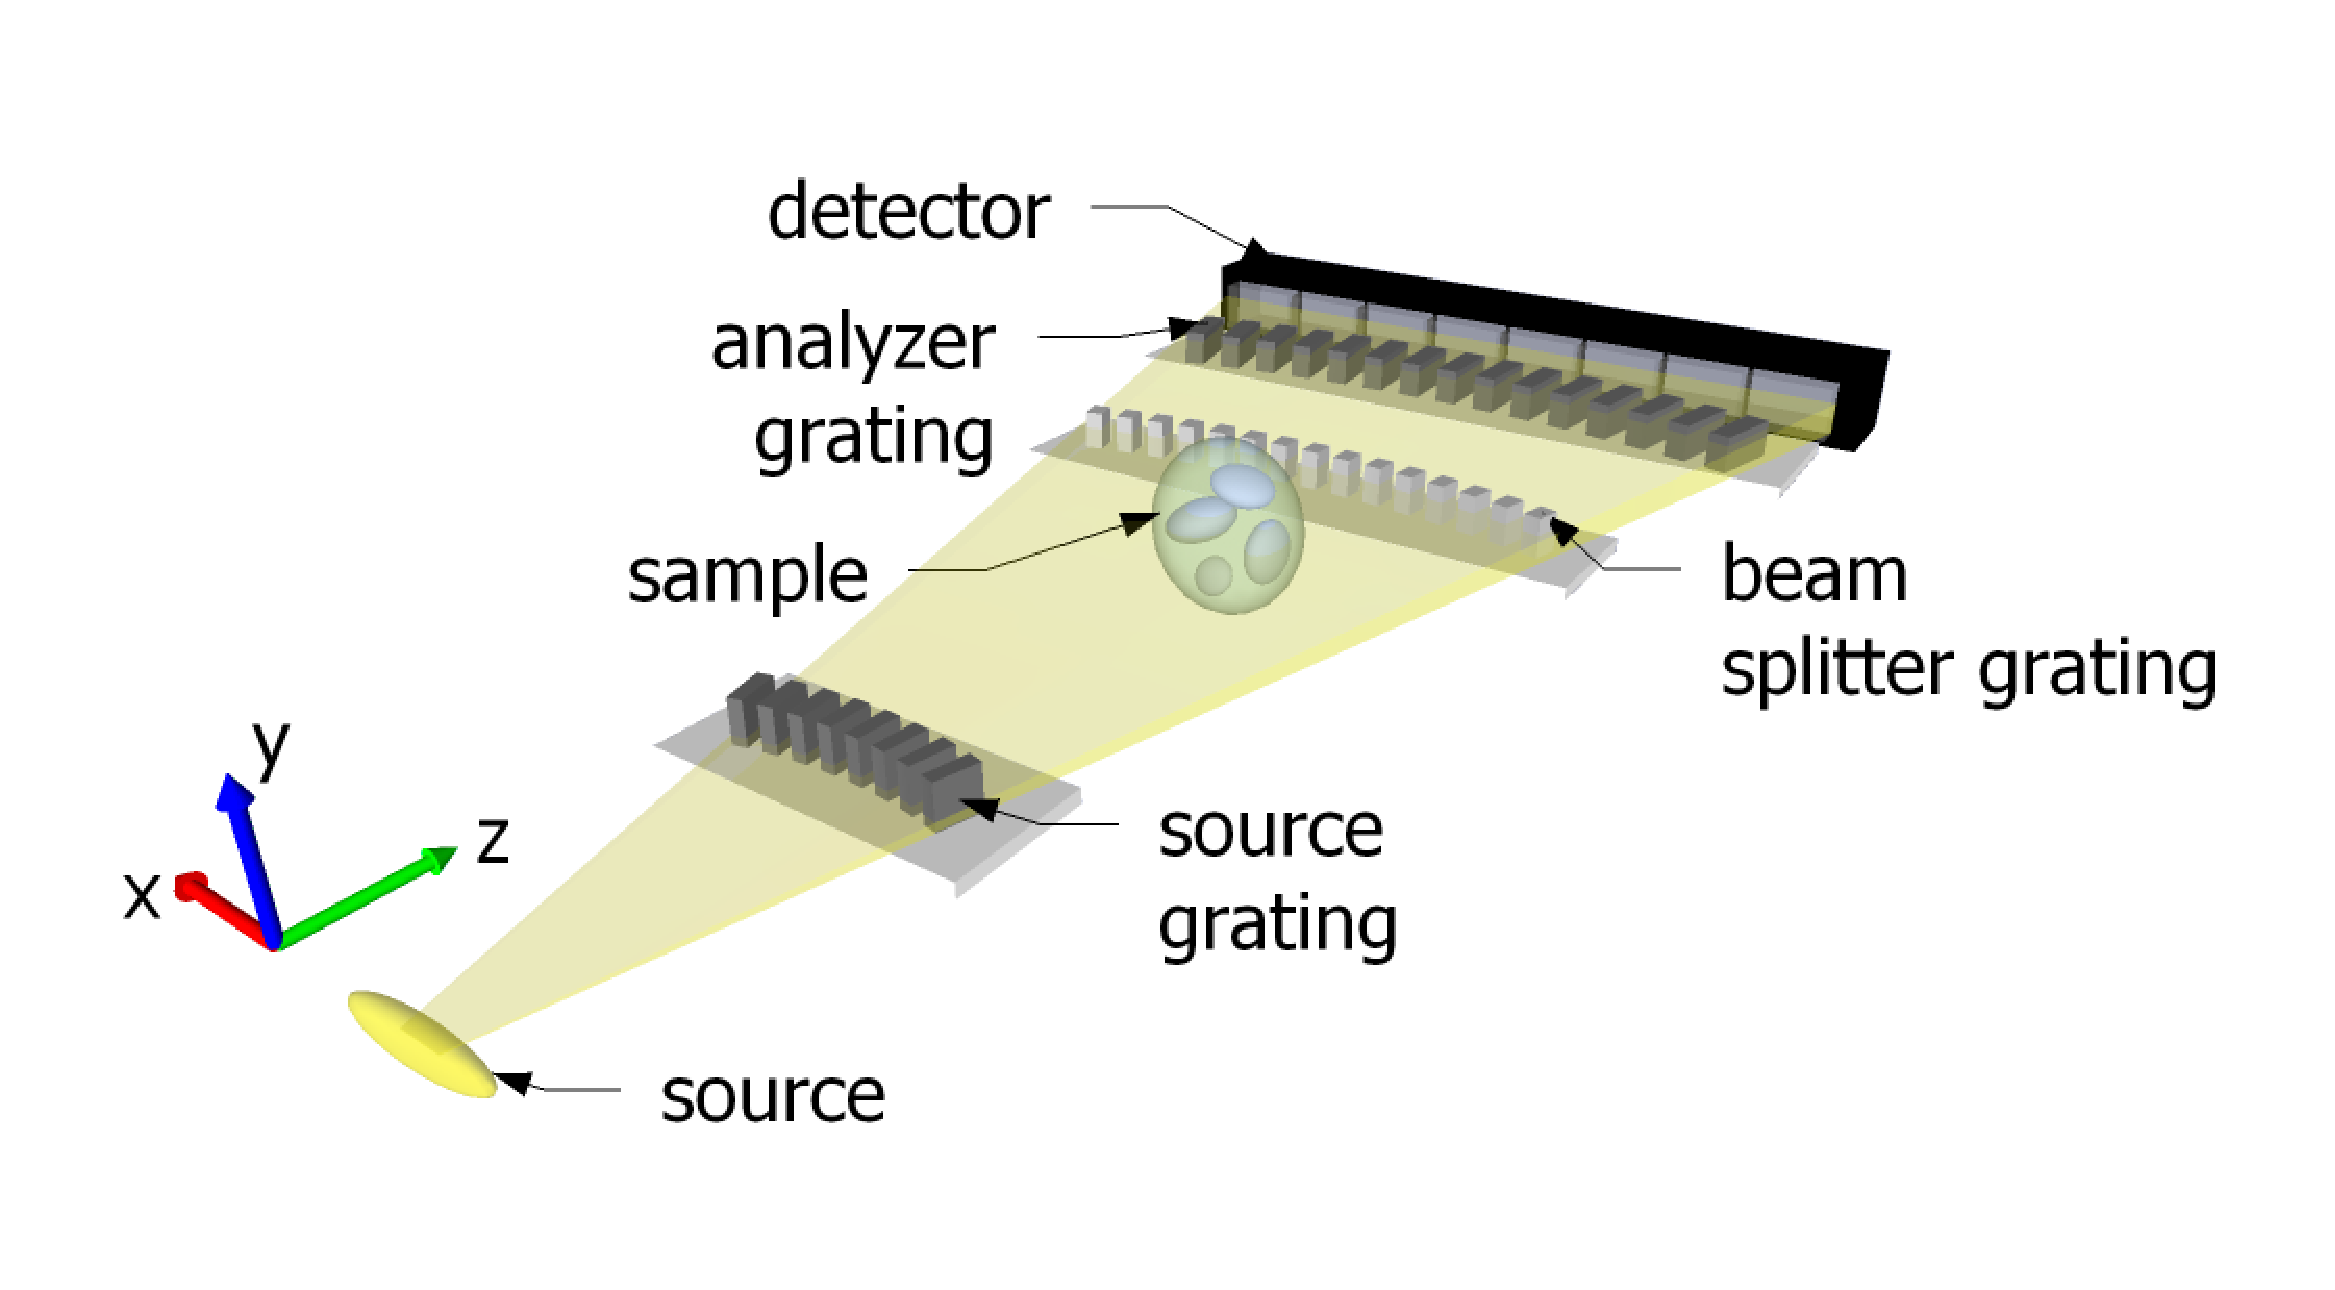
\includegraphics[width=\textwidth]{gfx/figure1.eps}
    \caption{Schematic of a grating
        interferometer for X-ray energies between 60 and
        \SI{150}{\kilo\electronvolt} in edge-on illumination mode. The
        aspect ratio is defined by the ratio of the traveling distance along the
        grating lines and the period and can be arbitrarily long. In order to maximize
        the field of view, the grating structures are aligned on an
        arc. A \SI{100}{\kilo\eV} setup was realized where the distance
        between the source and the source grating is \SI{23}{\centi\metre}
    and the distance between the source grating and the phase grating is
    \SI{16}{\centi\metre}. That is also the distance from the phase grating
to the analyzer grating.}%
\label{fig:schematic}
\end{figure}

Increasing the aspect ratio of the gratings typically leads to a reduction
of the field of view due to the change of the grating transmission function
at high incident angles. In order to overcome this problem, the grating
lines are circularly aligned with a radius equal to the distance to the
source. This allows to achieve an arbitrarily large field of view in a
fan-beam geometry, a significant improvement compared to face-on based and
glancing angle~\cite{Stutman2012a} approaches.
Face-on gratings can sometimes be manufactured on very thin silicon,
graphite or even titanium substrates\cn that can be bent to accomodate the beam
curvature at least in one direction for a two-dimensional setup. However,
this procedure involves the risk of destroying the grating if a too small
radius of curvature is chosen, or a defect in the substrate provokes a
crack.                                                

The combination of edge-on illumination and circularly aligned structures
enables phase-contrast imaging at arbitrary design energies and with a
maximum field of view in the horizontal direction ($x$ direction). These
advantages come at the expense of a limited field of view in the vertical
direction ($y$ direction), which is, depending on the X-ray detector,
typically a few pixels. However, radiographic 2D imaging can be obtained by
scanning the sample or a thin fan beam. The scanning technique has been
demonstrated to deliver less dose than the conventional approach based on
the illumination of a large area. In digital mammography, for instance,
where dose is a critical issue, Philips' MicroDose system combines a
scanning approach with an highly collimated fan beam~\cite{Aslund2007}.
Thanks to the high collimation, the dose deposited on  patients has been
reported to be significantly lower than with other instruments based on the
illumination of a large area detector~\cite{Oduko2010}. Similarly, for
tomographic images, the approach allows single slice \ac{CT} or full 3D
imaging in scanning mode.

Grating design and fabrication is nonstandard and involves a complex mask
design, as shown in Fig.~\ref{Fig:grating_mask}. Multiple gratings can
reside on a silicon chip with their specific structure length and curvature.
For the current experiments, a symmetric interferometer with a grating
period of $p = \SI{2.8}{\micro\metre}$ for all gratings has been used.

\subsection{Designing the grating parameters}
The grating parameters are chosen with the goal of optimizing the
sensitivity to the angle of refraction of X-rays, while keeping a compact
setup with a total length of about \SI{0.5}{\meter}.

The variance of the differential phase signal, with a Poisson variance of
the counts $\sigma_{\text{det}}^2$ in a detector pixel, is given by~\cite{Raupach2011}
\begin{equation}
    \sigma_\alpha = \frac{p_2}{\pi D_j}
    \frac{\sqrt{2}}{v}\sigma_{\text{det}}.\label{eq:variance}
\end{equation}
In order to obtain the maximum sensitivity it would be necessary to
fabricate gratings with a very small period
$p_2$, within technical constraint of the fabrication
techniques~\cite{David2007,Kenntner2010}.

For a constant total length $\ell + D_j$ of the interferometer, the factor
$p_2/D_j$ can be rewritten through~\eqref{eq:p0} in~\eqref{eq:variance}
\begin{equation*}
    \frac{p_2}{D_j} = \frac{p_0 + p_2}{\ell + D_j}.
\end{equation*}
The technical challenges for the fabrication of the two absorption gratings
\G0 and \G2 are obviously the same, therefore the maximum sensitivity is
achieved for the smallest achievable periods that are the same for both
gratings.

This is why we chose to realize symmetrical setups with $\ell = D_j'$ and $p_0 = p_1 = p_2$.

The second critical factor in~\eqref{eq:variance} is the visibility~$v$. The
variance is indeed not necessarily decreased by increasing the distance
$D_j$ for two reasons:
\begin{aenumerate}
    \item the relative noise introduced by the detector
        $\sigma_{\text{det}}/N$, for
        $N$ counts, is proportional to $1 / \sqrt{N}$, with the inverse
        square relationship $N \propto
        D_j^{-2}$
    \item the width of the spectrum positively contributing to the
        interference pattern decreases with distance according
        to~\eqref{eq:acceptance}. A theoretical maximum\cn of
        \SI{26}{\percent} for the first order $j = 1$ is reduced to
        $\SI{10}{\percent}$ for $j = 5$.
\end{aenumerate}
For this reason all interferometers are designed for the first Lohmann
distance $D_1 = p_1^2 / 8 \lambda$.

The design energy is $\SI{100}{\kilo\electronvolt}$ and the beam splitter
grating periodically shifts the phase by zero and $\pi$ at this
energy~\cite{David2002}. Using
gold as the phase shifting material, a structure length of
$h_1 = \SI{19.8}{\micro \metre}$ is required. The analyzer grating is an absorption mask
for sensing slight changes of the interference pattern generated by the beam
splitter~\cite{Momose2003a}. With a structure length of $h_2 =
\SI{800}{\micro \metre}$
it can absorb more than \SI{90}{\percent} of the incoming X-rays up to energies of 
$\SI{160}{\kilo\electronvolt}$. The beam splitter and analyzer grating are
separated at the first fractional Talbot order~\cite{Weitkamp2005},
resulting in an intergrating distance of $\SI{158}{\milli\metre}$. However,
the precise position of the analyzer grating along the beam axis is not
critical, and a change in visibility of less than \SI{1}{\percent} is
observed by displacing it by as much as \SI{5}{\milli\metre}. The
source grating splits the relatively large focal spot ($\sim
\SI{1}{\milli\metre}$) into an array of individually coherent, but mutually
incoherent sources~\cite{Pfeiffer2006}. It is also made of gold structures
with a length of $h_0 = h_2 = \SI{800}{\micro \metre}$.

A second setup has also been realized, for a design energy of
\SI{120}{\kilo\eV} with similar performance. All gratings are plated with
gold, with the exception of \G1 for the \SI{120}{\kilo\eV}
design energy, with a period of~\SI{2.8}{\micro\metre}, and an extension in
the vertical $y$ direction of~\SI{100}{\micro\metre}. The 
duty cycle is 0.5. The parameters are summarized in
table~\ref{tab:gratings}.

\begin{table}[htb]
    \centering
    \begin{tabular}{*4c}
        \toprule
        grating & design energy (\si{\kilo\eV}) & curvature radius
        (\si{\centi\metre}) & thickness (\si{\micro\metre}) \\
        \midrule
        $G_0$ & \num{100}/\num{120} & \num{23} & \num{800} \\
        $G_1$ & \num{100} & \num{38.8} & \num{42.2} \\
        $G_1$ & \num{120} & \num{42.0} & \num{19.4} \\
        $G_2$ & \num{100} & \num{54.5} & \num{800} \\
        $G_2$ & \num{120} & \num{60.9} & \num{800} \\
        \bottomrule
    \end{tabular}
    \caption{Parameters for the gratings of the two setups.}
    \label{tab:gratings}
\end{table}

\section{Alignment}
The interferometer has to be aligned on one plane in order to meet the
collimated fan beam with a precision of the order of~\SI{10}{\micro\metre}.
Moreover, the gratings have to match the design positions in space with
respect to the source, and be parallel to each other.
Each grating is mounted on goniometers with micrometric screws providing six
degrees of freedom, three for translation and three for rotation.
With figure~\ref{fig:schematic} as a reference, we report the repeatibility
figures that were effectively obtained in our experiments.
(table~\ref{tab:allineamento}).
\begin{table}[htb]
    \centering
    \begin{tabular}{*2c}
        \toprule
        alignment & repeatability\\
        \midrule
        rotation $x$ & \SI{0.05}{\degree}\\
        rotation $y$ & \SI{0.003}{\degree}\\
        rotation $z$ & \SI{0.05}{\degree}\\
        translation $x$ & \SI{1}{\milli\metre}\\
        translation $y$ & \SI{10}{\micro\metre}\\
        translation $z$ & \SI{5}{\milli\metre}\\
        \bottomrule
    \end{tabular}
    \caption{Repeatability figures for the alignment of each grating for six
    degrees of freedom.}
    \label{tab:allineamento}
\end{table}
The alignment protocol is more complex and time consuming than for a
two-dimensional grating interferometer since it is impossible to rely on
two-dimensional Moir\'e patterns as a guidance and it is necessary to scan
each grating on the collimated beam in order to understand its position.
The alignment steps are as follows:
\begin{enumerate}
    \item manual setting of the $z$ position of the gratings;
    \item alignment of the translation along $x$, with a previously
        calibrated laser;
    \item alignment of the translation along $y$,
        so that each grating is centered with respect to the center of the
        fan beam. This is achieved by moving each grating along the $y$ axis
        in small steps and noting in which position the grating enters and
        exits the fan beam during the scan. The middle point is then
        chosen;
    \item rotation around $z$ is fixed when the upper edge of each grating,
        as visible in an absorption scan, is parallel to a detector
        pixel (see figure~\ref{fig:alignment-z});
        \begin{figure}[htb]
            \centering
            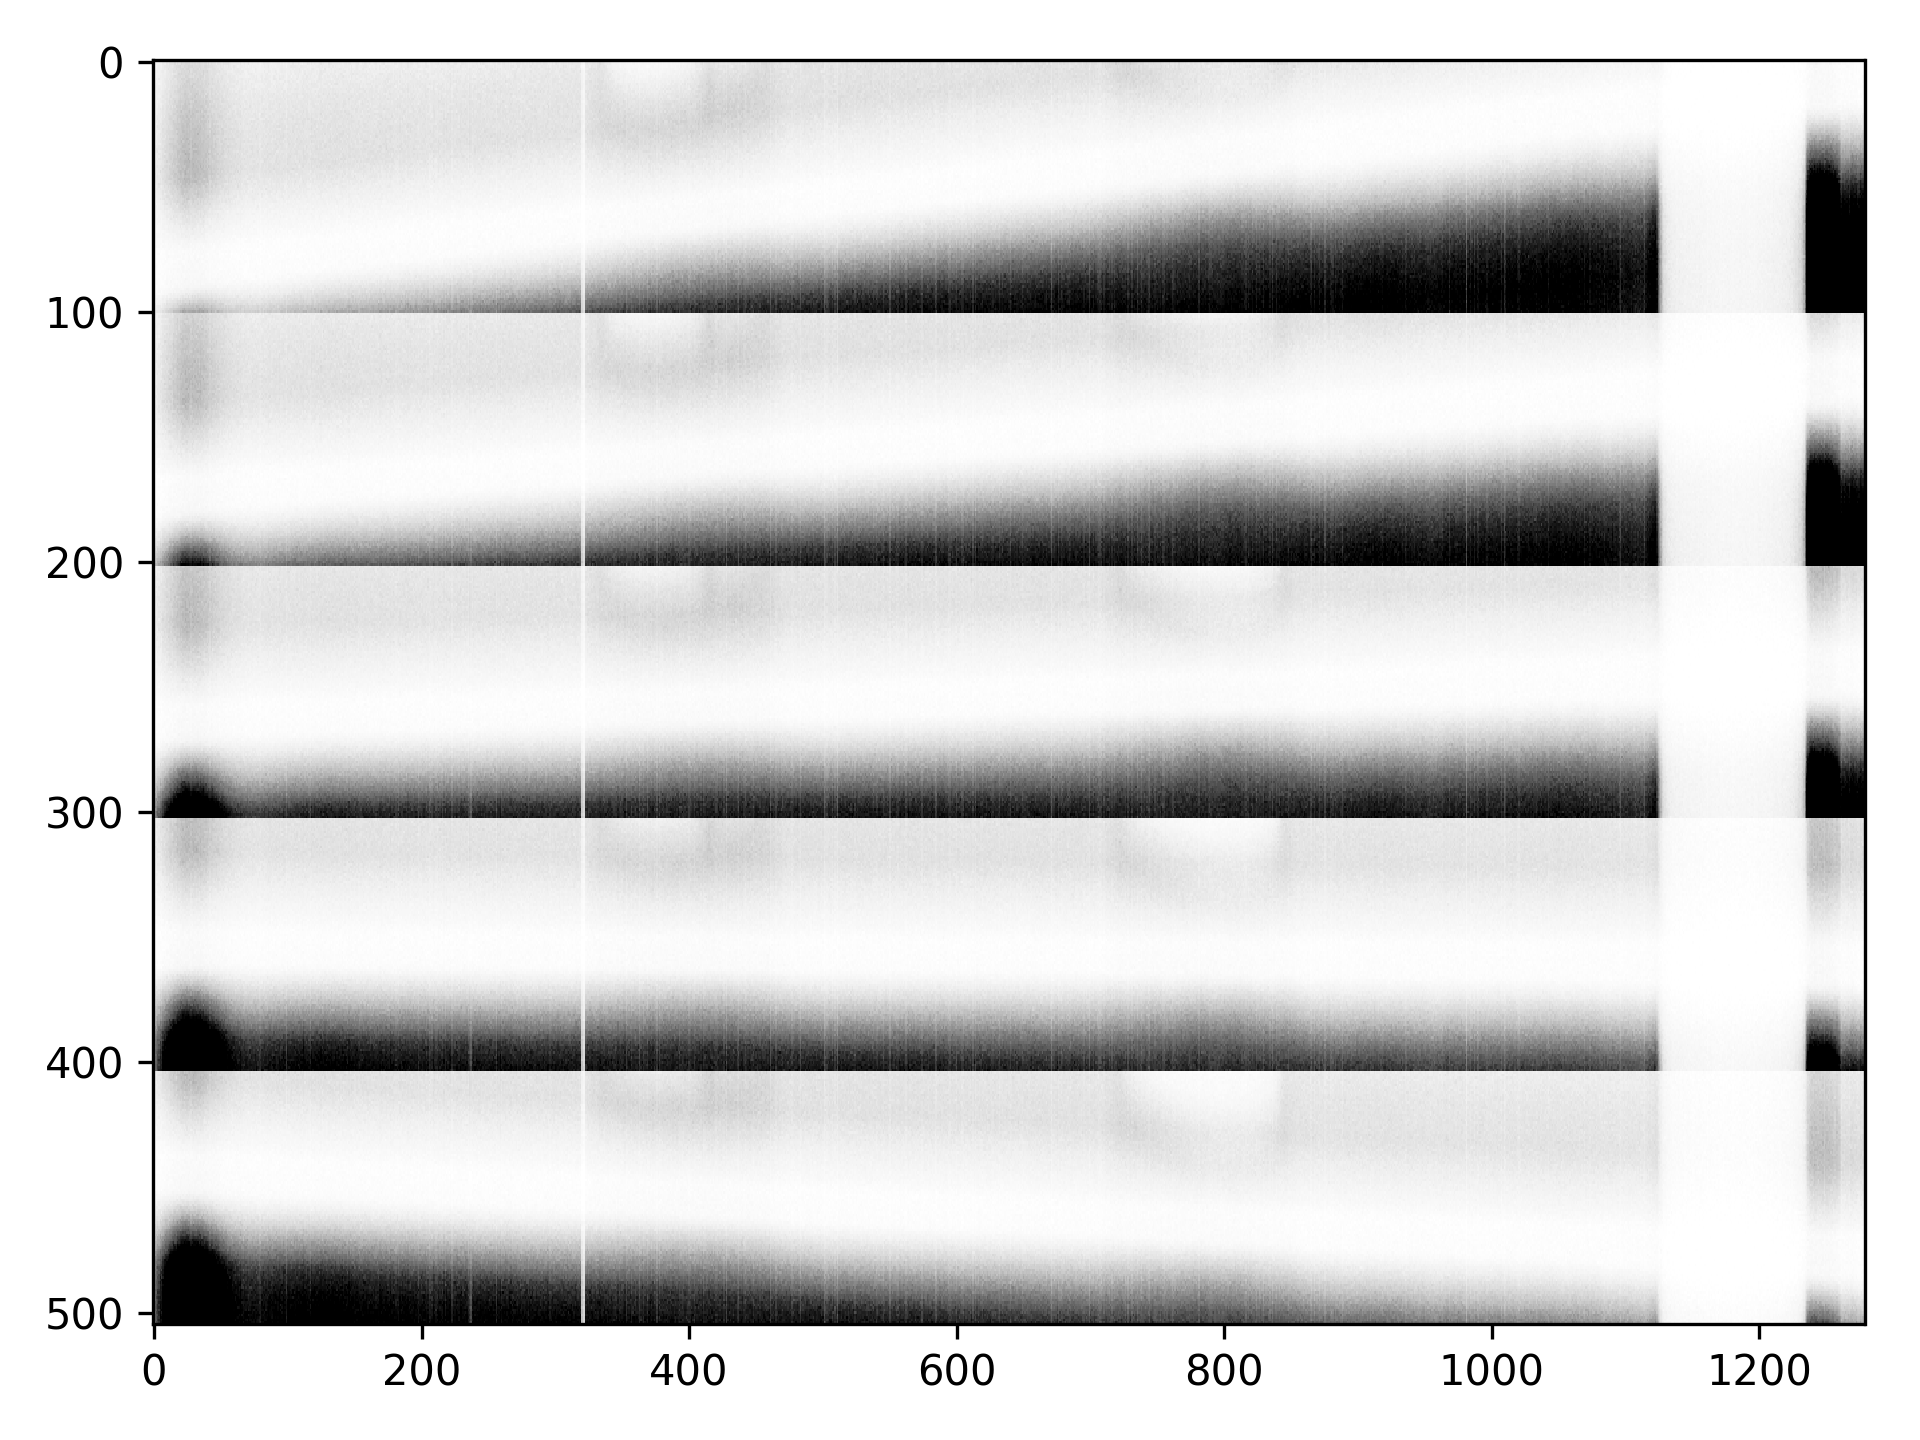
\includegraphics[width=\textwidth]{gfx/alignment-rot-z.png}
            \caption{Alignment of the \G2 grating with respect to the rotation
                around
            the beam axis $z$. The one-dimensional beam is scanned across the
            grating on a range of \SI{0.6}{\milli\metre}. This is repeated across
            five different positions of the rotation-$z$ motor from \num{-2} to
            \SI{+2}{\degree} in order to choose the
            best alignment, which in this case lies in an intermediate position between
            the fourth and fifth section from the top. The same scan is then repeated
        with finer steps in order to achieve a high precision in the alignment.}
            \label{fig:alignment-z}
        \end{figure}
    \item rotation around the $x$ axis is fixed by observing the appearance
        of the grating on a transmission image. It is best when the edges of
        the grating are defined and the area blocked by the grating itself
        appears smallest (see figure~\ref{fig:alignment-x});
        \begin{figure}[htb]
            \centering
            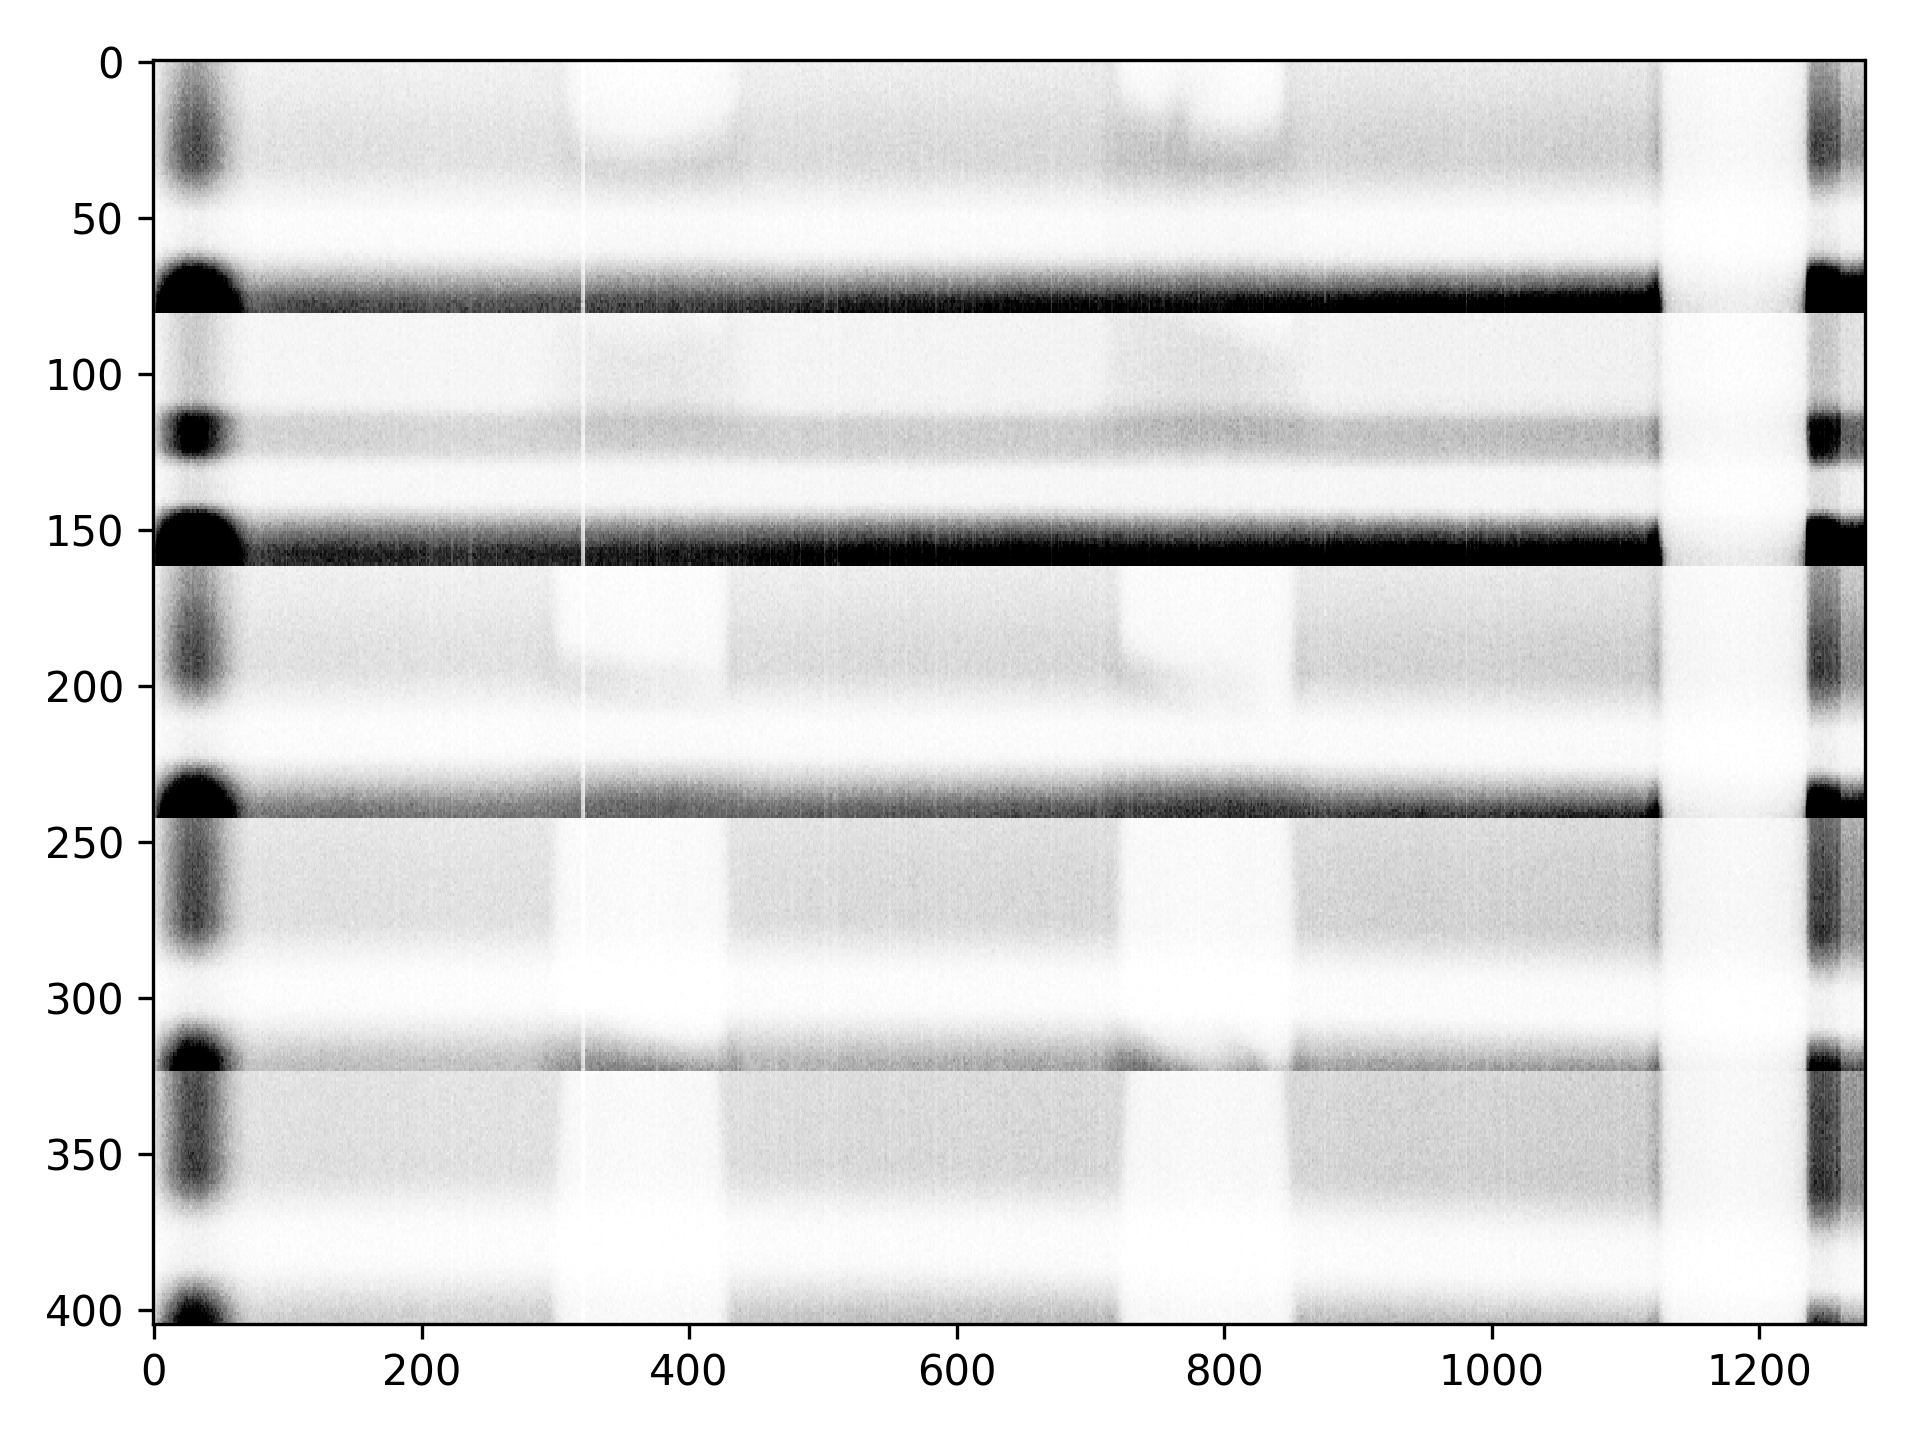
\includegraphics[width=\textwidth]{gfx/alignment-rot-x.png}
            \caption{Alignment of the \G2 grating with respect to the rotation
            around the $x$ axis. The one-dimensional beam is scanned across the
            grating on a range of \SI{0.6}{\milli\metre}. This is repeated across
            five different positions of the rotation-$x$ motor from \num{-1} to
            \SI{+1}{\degree} in order to choose the
            best alignment, this is achieved when the grating edges are well defined in
            the absorption picture and the grating appears thinnest, as in the second
        section from the top.}
            \label{fig:alignment-x}
        \end{figure}
    \item rotation around the $y$ and a fine translation along $z$ of the
        absorption gratings are fixed by maximizing the flux of X-rays
        through these two gratings.
    \item rotation along the $y$ axis and the position along $z$
        of \G{1} cannot be directly observed since the phase-shifting
        structures do not provide enough absorption to be visible.
        Moir\'e fringes are used to get the best alignment: the grating is
        best aligned when such fringes disappear;
    \item visibility scans with small excursions and fine steps
        ($\pm\SI{0.05}{\degree}$ and $\pm\SI{0.2}{\milli\meter}$) are
        performed for all degrees of freedom in order to apply small
        residual corrections: on each scan the location with maximum
        visibility is kept.
\end{enumerate}

\section{Performance}
The visibility of the systems, that is the ratio of the amplitude to the
mean value of the phase stepping curve, has an inverse proportionality with the
standard deviation of the refraction angle, according
to~\eqref{eq:variance}, and it is therefore the fundamental parameter to
characterize the performance of the experiment. It is unfortunately affected
by defects in the grating structures as shown by scanning electron
microscope investigations, with deformations (figure~\ref{fig:deformazioni})
and an incomplete electroplating (figure~\ref{fig:galvanizzazione})
negatively affecting the visibility.

\begin{figure}[htb]
    \centering
    \begin{subfigure}[b]{.49\textwidth}
    \centering
    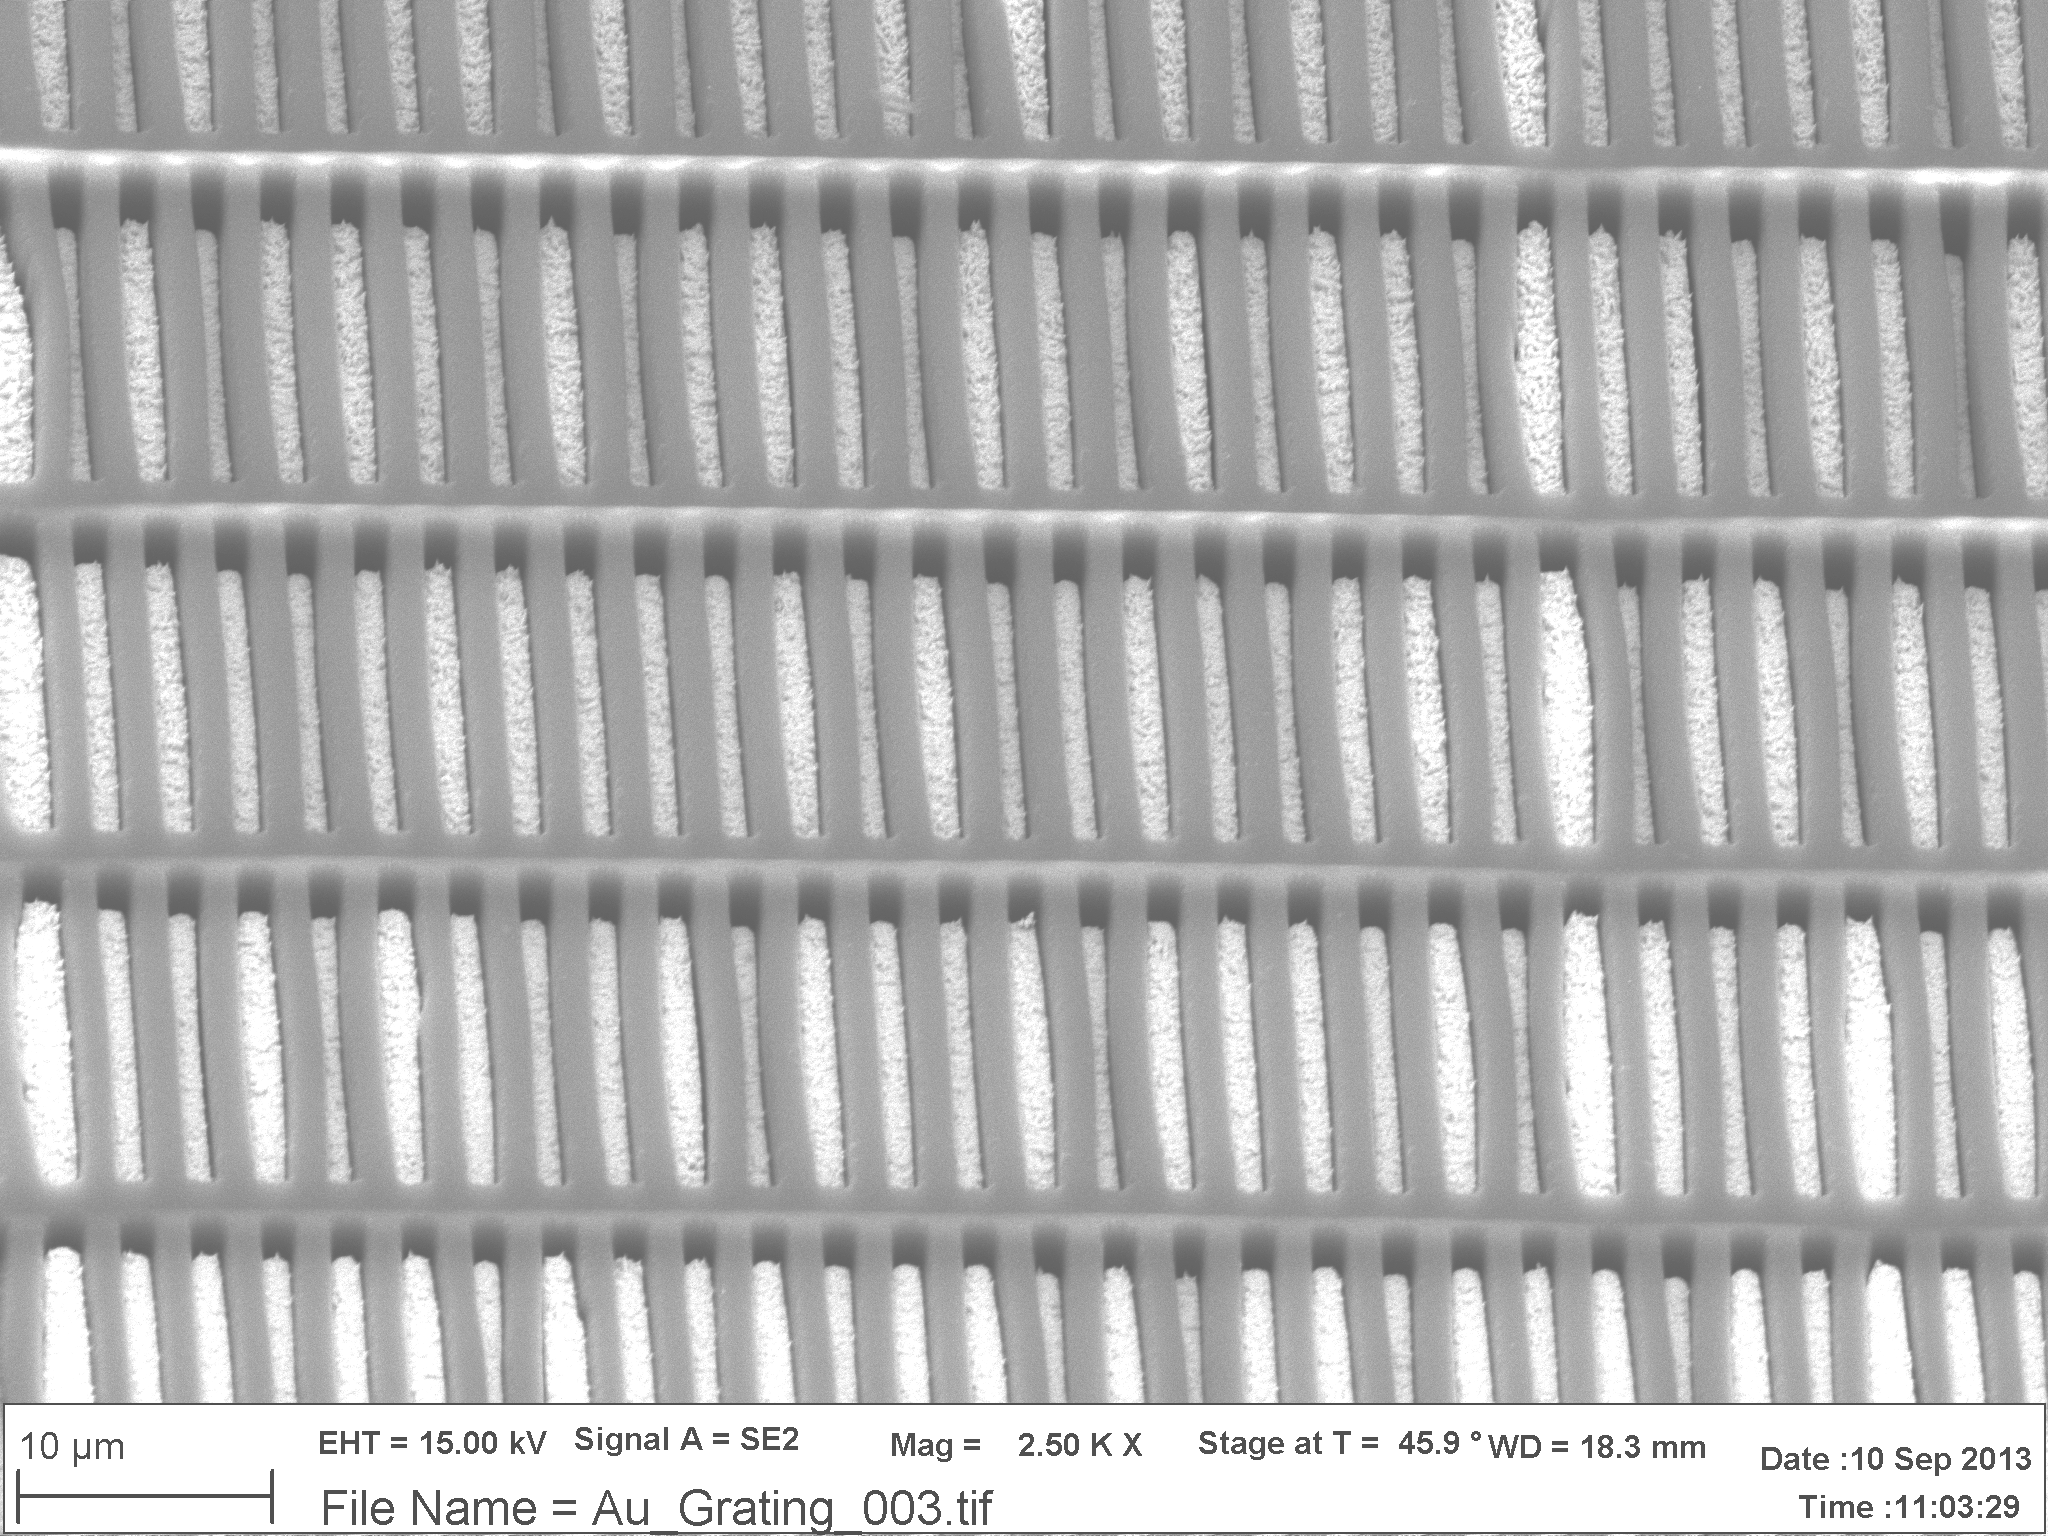
\includegraphics[width=\textwidth]{gfx/Au_Grating_003.png}
    \caption{}
    \label{fig:deformazioni}
    \end{subfigure}
    \hfill
    \begin{subfigure}[b]{.49\textwidth}
    \centering
    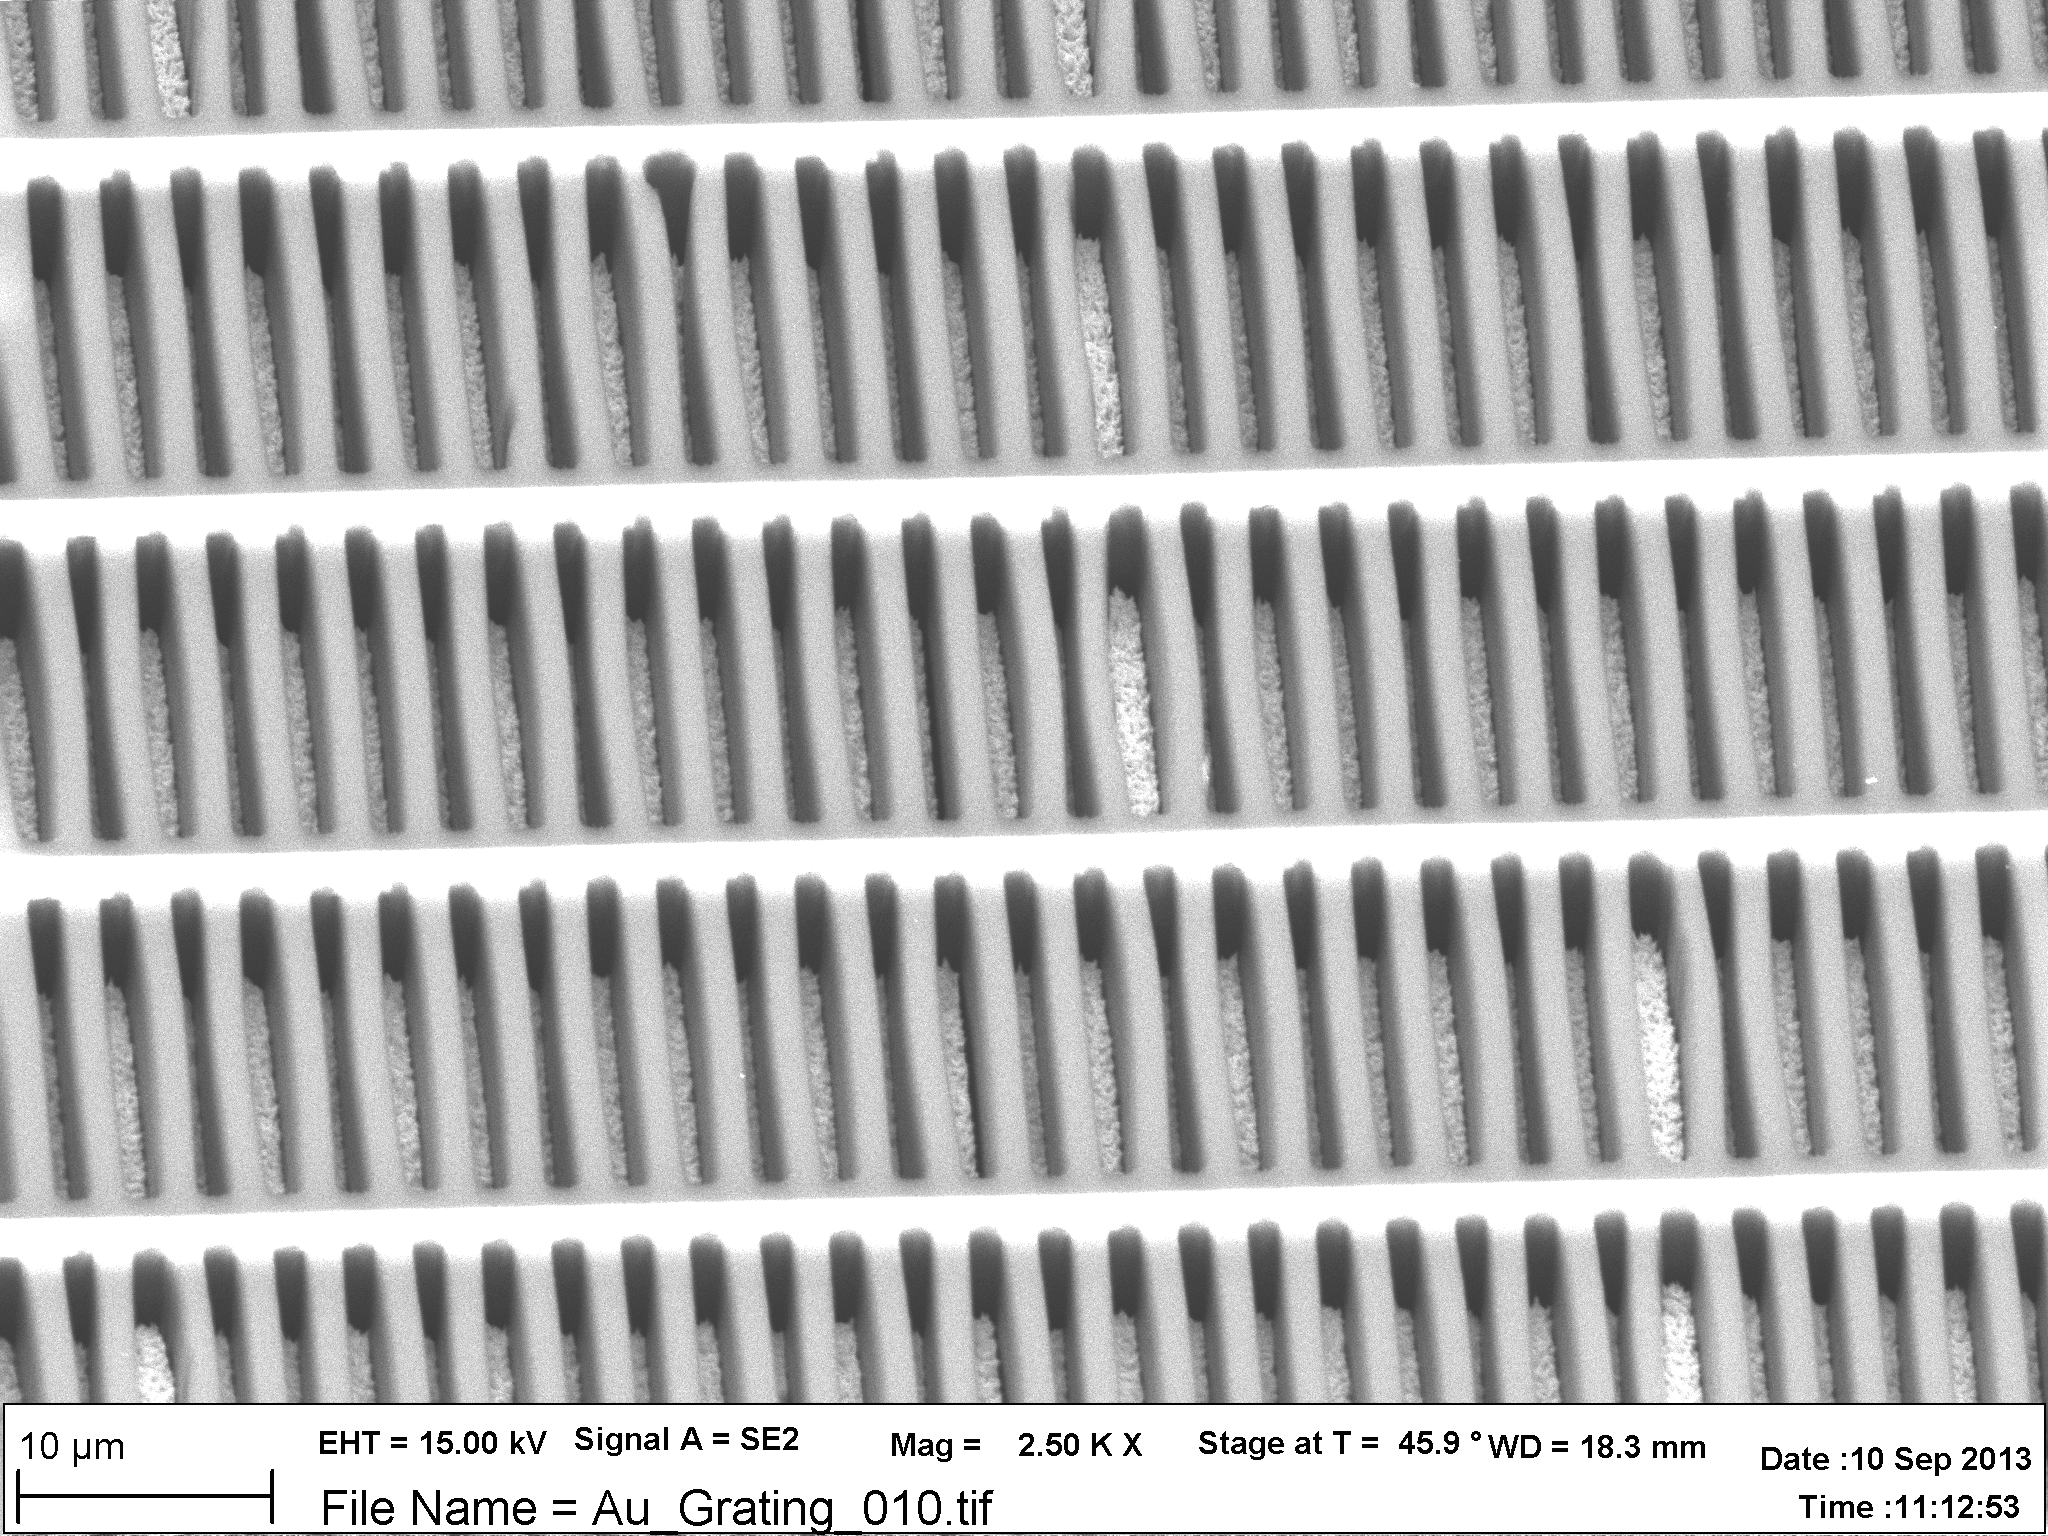
\includegraphics[width=\textwidth]{gfx/Au_Grating_010.png}
    \caption{}
    \label{fig:galvanizzazione}
    \end{subfigure}
    \caption[Electron microscope images of a gold grating.]{Scanning
        electron microscope images of a gold grating.
        Deformations in the grating lines~(\ref{fig:deformazioni}) and an
        incomplete electroplating~(\ref{fig:galvanizzazione}) can be seen.
    }
\end{figure}

Periodical variations in the visibility as a function of the transverse
position $x$ are usually related to residual Moir\'e fringes that could not
be eliminated through alignment. This is likely given by a mismatch in the
duty cycles of the gratings, that were measured as varying between 
\num{0.35} and \num{0.6}, with a significant deviation from the nominal value
of \num{0.5}.

The maximum visibility achieved by the two setups is shown in 
figure~\ref{fig:visibility100} and~\ref{fig:visibility120}, between \num{5} and
\SI{6}{\percent} on average.

\begin{figure}[htb]
    \centering
    %% Creator: Matplotlib, PGF backend
%%
%% To include the figure in your LaTeX document, write
%%   \input{<filename>.pgf}
%%
%% Make sure the required packages are loaded in your preamble
%%   \usepackage{pgf}
%%
%% Figures using additional raster images can only be included by \input if
%% they are in the same directory as the main LaTeX file. For loading figures
%% from other directories you can use the `import` package
%%   \usepackage{import}
%% and then include the figures with
%%   \import{<path to file>}{<filename>.pgf}
%%
%% Matplotlib used the following preamble
%%   \usepackage{fontspec}
%%
\begingroup%
\makeatletter%
\begin{pgfpicture}%
\pgfpathrectangle{\pgfpointorigin}{\pgfqpoint{4.600000in}{3.000000in}}%
\pgfusepath{use as bounding box, clip}%
\begin{pgfscope}%
\pgfsetbuttcap%
\pgfsetmiterjoin%
\definecolor{currentfill}{rgb}{1.000000,1.000000,1.000000}%
\pgfsetfillcolor{currentfill}%
\pgfsetlinewidth{0.000000pt}%
\definecolor{currentstroke}{rgb}{1.000000,1.000000,1.000000}%
\pgfsetstrokecolor{currentstroke}%
\pgfsetdash{}{0pt}%
\pgfpathmoveto{\pgfqpoint{0.000000in}{0.000000in}}%
\pgfpathlineto{\pgfqpoint{4.600000in}{0.000000in}}%
\pgfpathlineto{\pgfqpoint{4.600000in}{3.000000in}}%
\pgfpathlineto{\pgfqpoint{0.000000in}{3.000000in}}%
\pgfpathclose%
\pgfusepath{fill}%
\end{pgfscope}%
\begin{pgfscope}%
\pgfsetbuttcap%
\pgfsetmiterjoin%
\definecolor{currentfill}{rgb}{1.000000,1.000000,1.000000}%
\pgfsetfillcolor{currentfill}%
\pgfsetlinewidth{0.000000pt}%
\definecolor{currentstroke}{rgb}{0.000000,0.000000,0.000000}%
\pgfsetstrokecolor{currentstroke}%
\pgfsetstrokeopacity{0.000000}%
\pgfsetdash{}{0pt}%
\pgfpathmoveto{\pgfqpoint{0.765083in}{0.609944in}}%
\pgfpathlineto{\pgfqpoint{4.400000in}{0.609944in}}%
\pgfpathlineto{\pgfqpoint{4.400000in}{2.783471in}}%
\pgfpathlineto{\pgfqpoint{0.765083in}{2.783471in}}%
\pgfpathclose%
\pgfusepath{fill}%
\end{pgfscope}%
\begin{pgfscope}%
\pgfsetbuttcap%
\pgfsetroundjoin%
\definecolor{currentfill}{rgb}{0.000000,0.000000,0.000000}%
\pgfsetfillcolor{currentfill}%
\pgfsetlinewidth{0.803000pt}%
\definecolor{currentstroke}{rgb}{0.000000,0.000000,0.000000}%
\pgfsetstrokecolor{currentstroke}%
\pgfsetdash{}{0pt}%
\pgfsys@defobject{currentmarker}{\pgfqpoint{0.000000in}{-0.048611in}}{\pgfqpoint{0.000000in}{0.000000in}}{%
\pgfpathmoveto{\pgfqpoint{0.000000in}{0.000000in}}%
\pgfpathlineto{\pgfqpoint{0.000000in}{-0.048611in}}%
\pgfusepath{stroke,fill}%
}%
\begin{pgfscope}%
\pgfsys@transformshift{0.930307in}{0.609944in}%
\pgfsys@useobject{currentmarker}{}%
\end{pgfscope}%
\end{pgfscope}%
\begin{pgfscope}%
\pgftext[x=0.930307in,y=0.491889in,,top]{\rmfamily\fontsize{11.000000}{13.200000}\selectfont 300}%
\end{pgfscope}%
\begin{pgfscope}%
\pgfsetbuttcap%
\pgfsetroundjoin%
\definecolor{currentfill}{rgb}{0.000000,0.000000,0.000000}%
\pgfsetfillcolor{currentfill}%
\pgfsetlinewidth{0.803000pt}%
\definecolor{currentstroke}{rgb}{0.000000,0.000000,0.000000}%
\pgfsetstrokecolor{currentstroke}%
\pgfsetdash{}{0pt}%
\pgfsys@defobject{currentmarker}{\pgfqpoint{0.000000in}{-0.048611in}}{\pgfqpoint{0.000000in}{0.000000in}}{%
\pgfpathmoveto{\pgfqpoint{0.000000in}{0.000000in}}%
\pgfpathlineto{\pgfqpoint{0.000000in}{-0.048611in}}%
\pgfusepath{stroke,fill}%
}%
\begin{pgfscope}%
\pgfsys@transformshift{1.592525in}{0.609944in}%
\pgfsys@useobject{currentmarker}{}%
\end{pgfscope}%
\end{pgfscope}%
\begin{pgfscope}%
\pgftext[x=1.592525in,y=0.491889in,,top]{\rmfamily\fontsize{11.000000}{13.200000}\selectfont 400}%
\end{pgfscope}%
\begin{pgfscope}%
\pgfsetbuttcap%
\pgfsetroundjoin%
\definecolor{currentfill}{rgb}{0.000000,0.000000,0.000000}%
\pgfsetfillcolor{currentfill}%
\pgfsetlinewidth{0.803000pt}%
\definecolor{currentstroke}{rgb}{0.000000,0.000000,0.000000}%
\pgfsetstrokecolor{currentstroke}%
\pgfsetdash{}{0pt}%
\pgfsys@defobject{currentmarker}{\pgfqpoint{0.000000in}{-0.048611in}}{\pgfqpoint{0.000000in}{0.000000in}}{%
\pgfpathmoveto{\pgfqpoint{0.000000in}{0.000000in}}%
\pgfpathlineto{\pgfqpoint{0.000000in}{-0.048611in}}%
\pgfusepath{stroke,fill}%
}%
\begin{pgfscope}%
\pgfsys@transformshift{2.254743in}{0.609944in}%
\pgfsys@useobject{currentmarker}{}%
\end{pgfscope}%
\end{pgfscope}%
\begin{pgfscope}%
\pgftext[x=2.254743in,y=0.491889in,,top]{\rmfamily\fontsize{11.000000}{13.200000}\selectfont 500}%
\end{pgfscope}%
\begin{pgfscope}%
\pgfsetbuttcap%
\pgfsetroundjoin%
\definecolor{currentfill}{rgb}{0.000000,0.000000,0.000000}%
\pgfsetfillcolor{currentfill}%
\pgfsetlinewidth{0.803000pt}%
\definecolor{currentstroke}{rgb}{0.000000,0.000000,0.000000}%
\pgfsetstrokecolor{currentstroke}%
\pgfsetdash{}{0pt}%
\pgfsys@defobject{currentmarker}{\pgfqpoint{0.000000in}{-0.048611in}}{\pgfqpoint{0.000000in}{0.000000in}}{%
\pgfpathmoveto{\pgfqpoint{0.000000in}{0.000000in}}%
\pgfpathlineto{\pgfqpoint{0.000000in}{-0.048611in}}%
\pgfusepath{stroke,fill}%
}%
\begin{pgfscope}%
\pgfsys@transformshift{2.916962in}{0.609944in}%
\pgfsys@useobject{currentmarker}{}%
\end{pgfscope}%
\end{pgfscope}%
\begin{pgfscope}%
\pgftext[x=2.916962in,y=0.491889in,,top]{\rmfamily\fontsize{11.000000}{13.200000}\selectfont 600}%
\end{pgfscope}%
\begin{pgfscope}%
\pgfsetbuttcap%
\pgfsetroundjoin%
\definecolor{currentfill}{rgb}{0.000000,0.000000,0.000000}%
\pgfsetfillcolor{currentfill}%
\pgfsetlinewidth{0.803000pt}%
\definecolor{currentstroke}{rgb}{0.000000,0.000000,0.000000}%
\pgfsetstrokecolor{currentstroke}%
\pgfsetdash{}{0pt}%
\pgfsys@defobject{currentmarker}{\pgfqpoint{0.000000in}{-0.048611in}}{\pgfqpoint{0.000000in}{0.000000in}}{%
\pgfpathmoveto{\pgfqpoint{0.000000in}{0.000000in}}%
\pgfpathlineto{\pgfqpoint{0.000000in}{-0.048611in}}%
\pgfusepath{stroke,fill}%
}%
\begin{pgfscope}%
\pgfsys@transformshift{3.579180in}{0.609944in}%
\pgfsys@useobject{currentmarker}{}%
\end{pgfscope}%
\end{pgfscope}%
\begin{pgfscope}%
\pgftext[x=3.579180in,y=0.491889in,,top]{\rmfamily\fontsize{11.000000}{13.200000}\selectfont 700}%
\end{pgfscope}%
\begin{pgfscope}%
\pgfsetbuttcap%
\pgfsetroundjoin%
\definecolor{currentfill}{rgb}{0.000000,0.000000,0.000000}%
\pgfsetfillcolor{currentfill}%
\pgfsetlinewidth{0.803000pt}%
\definecolor{currentstroke}{rgb}{0.000000,0.000000,0.000000}%
\pgfsetstrokecolor{currentstroke}%
\pgfsetdash{}{0pt}%
\pgfsys@defobject{currentmarker}{\pgfqpoint{0.000000in}{-0.048611in}}{\pgfqpoint{0.000000in}{0.000000in}}{%
\pgfpathmoveto{\pgfqpoint{0.000000in}{0.000000in}}%
\pgfpathlineto{\pgfqpoint{0.000000in}{-0.048611in}}%
\pgfusepath{stroke,fill}%
}%
\begin{pgfscope}%
\pgfsys@transformshift{4.241399in}{0.609944in}%
\pgfsys@useobject{currentmarker}{}%
\end{pgfscope}%
\end{pgfscope}%
\begin{pgfscope}%
\pgftext[x=4.241399in,y=0.491889in,,top]{\rmfamily\fontsize{11.000000}{13.200000}\selectfont 800}%
\end{pgfscope}%
\begin{pgfscope}%
\pgftext[x=2.582542in,y=0.300667in,,top]{\rmfamily\fontsize{11.000000}{13.200000}\selectfont pixel}%
\end{pgfscope}%
\begin{pgfscope}%
\pgfsetbuttcap%
\pgfsetroundjoin%
\definecolor{currentfill}{rgb}{0.000000,0.000000,0.000000}%
\pgfsetfillcolor{currentfill}%
\pgfsetlinewidth{0.803000pt}%
\definecolor{currentstroke}{rgb}{0.000000,0.000000,0.000000}%
\pgfsetstrokecolor{currentstroke}%
\pgfsetdash{}{0pt}%
\pgfsys@defobject{currentmarker}{\pgfqpoint{-0.048611in}{0.000000in}}{\pgfqpoint{0.000000in}{0.000000in}}{%
\pgfpathmoveto{\pgfqpoint{0.000000in}{0.000000in}}%
\pgfpathlineto{\pgfqpoint{-0.048611in}{0.000000in}}%
\pgfusepath{stroke,fill}%
}%
\begin{pgfscope}%
\pgfsys@transformshift{0.765083in}{0.609944in}%
\pgfsys@useobject{currentmarker}{}%
\end{pgfscope}%
\end{pgfscope}%
\begin{pgfscope}%
\pgftext[x=0.447500in,y=0.556930in,left,base]{\rmfamily\fontsize{11.000000}{13.200000}\selectfont 0\%}%
\end{pgfscope}%
\begin{pgfscope}%
\pgfsetbuttcap%
\pgfsetroundjoin%
\definecolor{currentfill}{rgb}{0.000000,0.000000,0.000000}%
\pgfsetfillcolor{currentfill}%
\pgfsetlinewidth{0.803000pt}%
\definecolor{currentstroke}{rgb}{0.000000,0.000000,0.000000}%
\pgfsetstrokecolor{currentstroke}%
\pgfsetdash{}{0pt}%
\pgfsys@defobject{currentmarker}{\pgfqpoint{-0.048611in}{0.000000in}}{\pgfqpoint{0.000000in}{0.000000in}}{%
\pgfpathmoveto{\pgfqpoint{0.000000in}{0.000000in}}%
\pgfpathlineto{\pgfqpoint{-0.048611in}{0.000000in}}%
\pgfusepath{stroke,fill}%
}%
\begin{pgfscope}%
\pgfsys@transformshift{0.765083in}{0.971966in}%
\pgfsys@useobject{currentmarker}{}%
\end{pgfscope}%
\end{pgfscope}%
\begin{pgfscope}%
\pgftext[x=0.447500in,y=0.918952in,left,base]{\rmfamily\fontsize{11.000000}{13.200000}\selectfont 2\%}%
\end{pgfscope}%
\begin{pgfscope}%
\pgfsetbuttcap%
\pgfsetroundjoin%
\definecolor{currentfill}{rgb}{0.000000,0.000000,0.000000}%
\pgfsetfillcolor{currentfill}%
\pgfsetlinewidth{0.803000pt}%
\definecolor{currentstroke}{rgb}{0.000000,0.000000,0.000000}%
\pgfsetstrokecolor{currentstroke}%
\pgfsetdash{}{0pt}%
\pgfsys@defobject{currentmarker}{\pgfqpoint{-0.048611in}{0.000000in}}{\pgfqpoint{0.000000in}{0.000000in}}{%
\pgfpathmoveto{\pgfqpoint{0.000000in}{0.000000in}}%
\pgfpathlineto{\pgfqpoint{-0.048611in}{0.000000in}}%
\pgfusepath{stroke,fill}%
}%
\begin{pgfscope}%
\pgfsys@transformshift{0.765083in}{1.333987in}%
\pgfsys@useobject{currentmarker}{}%
\end{pgfscope}%
\end{pgfscope}%
\begin{pgfscope}%
\pgftext[x=0.447500in,y=1.280973in,left,base]{\rmfamily\fontsize{11.000000}{13.200000}\selectfont 4\%}%
\end{pgfscope}%
\begin{pgfscope}%
\pgfsetbuttcap%
\pgfsetroundjoin%
\definecolor{currentfill}{rgb}{0.000000,0.000000,0.000000}%
\pgfsetfillcolor{currentfill}%
\pgfsetlinewidth{0.803000pt}%
\definecolor{currentstroke}{rgb}{0.000000,0.000000,0.000000}%
\pgfsetstrokecolor{currentstroke}%
\pgfsetdash{}{0pt}%
\pgfsys@defobject{currentmarker}{\pgfqpoint{-0.048611in}{0.000000in}}{\pgfqpoint{0.000000in}{0.000000in}}{%
\pgfpathmoveto{\pgfqpoint{0.000000in}{0.000000in}}%
\pgfpathlineto{\pgfqpoint{-0.048611in}{0.000000in}}%
\pgfusepath{stroke,fill}%
}%
\begin{pgfscope}%
\pgfsys@transformshift{0.765083in}{1.696009in}%
\pgfsys@useobject{currentmarker}{}%
\end{pgfscope}%
\end{pgfscope}%
\begin{pgfscope}%
\pgftext[x=0.447500in,y=1.642995in,left,base]{\rmfamily\fontsize{11.000000}{13.200000}\selectfont 6\%}%
\end{pgfscope}%
\begin{pgfscope}%
\pgfsetbuttcap%
\pgfsetroundjoin%
\definecolor{currentfill}{rgb}{0.000000,0.000000,0.000000}%
\pgfsetfillcolor{currentfill}%
\pgfsetlinewidth{0.803000pt}%
\definecolor{currentstroke}{rgb}{0.000000,0.000000,0.000000}%
\pgfsetstrokecolor{currentstroke}%
\pgfsetdash{}{0pt}%
\pgfsys@defobject{currentmarker}{\pgfqpoint{-0.048611in}{0.000000in}}{\pgfqpoint{0.000000in}{0.000000in}}{%
\pgfpathmoveto{\pgfqpoint{0.000000in}{0.000000in}}%
\pgfpathlineto{\pgfqpoint{-0.048611in}{0.000000in}}%
\pgfusepath{stroke,fill}%
}%
\begin{pgfscope}%
\pgfsys@transformshift{0.765083in}{2.058031in}%
\pgfsys@useobject{currentmarker}{}%
\end{pgfscope}%
\end{pgfscope}%
\begin{pgfscope}%
\pgftext[x=0.447500in,y=2.005017in,left,base]{\rmfamily\fontsize{11.000000}{13.200000}\selectfont 8\%}%
\end{pgfscope}%
\begin{pgfscope}%
\pgfsetbuttcap%
\pgfsetroundjoin%
\definecolor{currentfill}{rgb}{0.000000,0.000000,0.000000}%
\pgfsetfillcolor{currentfill}%
\pgfsetlinewidth{0.803000pt}%
\definecolor{currentstroke}{rgb}{0.000000,0.000000,0.000000}%
\pgfsetstrokecolor{currentstroke}%
\pgfsetdash{}{0pt}%
\pgfsys@defobject{currentmarker}{\pgfqpoint{-0.048611in}{0.000000in}}{\pgfqpoint{0.000000in}{0.000000in}}{%
\pgfpathmoveto{\pgfqpoint{0.000000in}{0.000000in}}%
\pgfpathlineto{\pgfqpoint{-0.048611in}{0.000000in}}%
\pgfusepath{stroke,fill}%
}%
\begin{pgfscope}%
\pgfsys@transformshift{0.765083in}{2.420052in}%
\pgfsys@useobject{currentmarker}{}%
\end{pgfscope}%
\end{pgfscope}%
\begin{pgfscope}%
\pgftext[x=0.372639in,y=2.367038in,left,base]{\rmfamily\fontsize{11.000000}{13.200000}\selectfont 10\%}%
\end{pgfscope}%
\begin{pgfscope}%
\pgfsetbuttcap%
\pgfsetroundjoin%
\definecolor{currentfill}{rgb}{0.000000,0.000000,0.000000}%
\pgfsetfillcolor{currentfill}%
\pgfsetlinewidth{0.803000pt}%
\definecolor{currentstroke}{rgb}{0.000000,0.000000,0.000000}%
\pgfsetstrokecolor{currentstroke}%
\pgfsetdash{}{0pt}%
\pgfsys@defobject{currentmarker}{\pgfqpoint{-0.048611in}{0.000000in}}{\pgfqpoint{0.000000in}{0.000000in}}{%
\pgfpathmoveto{\pgfqpoint{0.000000in}{0.000000in}}%
\pgfpathlineto{\pgfqpoint{-0.048611in}{0.000000in}}%
\pgfusepath{stroke,fill}%
}%
\begin{pgfscope}%
\pgfsys@transformshift{0.765083in}{2.782074in}%
\pgfsys@useobject{currentmarker}{}%
\end{pgfscope}%
\end{pgfscope}%
\begin{pgfscope}%
\pgftext[x=0.372639in,y=2.729060in,left,base]{\rmfamily\fontsize{11.000000}{13.200000}\selectfont 12\%}%
\end{pgfscope}%
\begin{pgfscope}%
\pgftext[x=0.317083in,y=1.696707in,,bottom,rotate=90.000000]{\rmfamily\fontsize{11.000000}{13.200000}\selectfont \(\displaystyle v = 2 a_1 / a_0\)}%
\end{pgfscope}%
\begin{pgfscope}%
\pgfpathrectangle{\pgfqpoint{0.765083in}{0.609944in}}{\pgfqpoint{3.634917in}{2.173527in}}%
\pgfusepath{clip}%
\pgfsetrectcap%
\pgfsetroundjoin%
\pgfsetlinewidth{1.003750pt}%
\definecolor{currentstroke}{rgb}{0.000000,0.000000,0.000000}%
\pgfsetstrokecolor{currentstroke}%
\pgfsetdash{}{0pt}%
\pgfpathmoveto{\pgfqpoint{0.930307in}{1.490811in}}%
\pgfpathlineto{\pgfqpoint{0.936929in}{1.542939in}}%
\pgfpathlineto{\pgfqpoint{0.943551in}{1.605378in}}%
\pgfpathlineto{\pgfqpoint{0.956795in}{1.881676in}}%
\pgfpathlineto{\pgfqpoint{0.963418in}{1.958687in}}%
\pgfpathlineto{\pgfqpoint{0.970040in}{1.951752in}}%
\pgfpathlineto{\pgfqpoint{0.976662in}{1.963687in}}%
\pgfpathlineto{\pgfqpoint{0.983284in}{1.962417in}}%
\pgfpathlineto{\pgfqpoint{0.989906in}{1.942207in}}%
\pgfpathlineto{\pgfqpoint{0.996529in}{1.960010in}}%
\pgfpathlineto{\pgfqpoint{1.003151in}{1.952079in}}%
\pgfpathlineto{\pgfqpoint{1.009773in}{1.933400in}}%
\pgfpathlineto{\pgfqpoint{1.016395in}{1.944024in}}%
\pgfpathlineto{\pgfqpoint{1.023017in}{1.884788in}}%
\pgfpathlineto{\pgfqpoint{1.029639in}{1.874021in}}%
\pgfpathlineto{\pgfqpoint{1.036262in}{1.801064in}}%
\pgfpathlineto{\pgfqpoint{1.042884in}{1.775372in}}%
\pgfpathlineto{\pgfqpoint{1.056128in}{1.668671in}}%
\pgfpathlineto{\pgfqpoint{1.062750in}{1.628183in}}%
\pgfpathlineto{\pgfqpoint{1.075995in}{1.503872in}}%
\pgfpathlineto{\pgfqpoint{1.082617in}{1.472177in}}%
\pgfpathlineto{\pgfqpoint{1.089239in}{1.467575in}}%
\pgfpathlineto{\pgfqpoint{1.095861in}{1.493243in}}%
\pgfpathlineto{\pgfqpoint{1.102483in}{1.487191in}}%
\pgfpathlineto{\pgfqpoint{1.109106in}{1.472698in}}%
\pgfpathlineto{\pgfqpoint{1.115728in}{1.500571in}}%
\pgfpathlineto{\pgfqpoint{1.122350in}{1.533998in}}%
\pgfpathlineto{\pgfqpoint{1.128972in}{1.556978in}}%
\pgfpathlineto{\pgfqpoint{1.135594in}{1.621151in}}%
\pgfpathlineto{\pgfqpoint{1.142217in}{1.614327in}}%
\pgfpathlineto{\pgfqpoint{1.148839in}{1.671261in}}%
\pgfpathlineto{\pgfqpoint{1.162083in}{1.595977in}}%
\pgfpathlineto{\pgfqpoint{1.168705in}{1.657572in}}%
\pgfpathlineto{\pgfqpoint{1.175327in}{1.740809in}}%
\pgfpathlineto{\pgfqpoint{1.181950in}{1.786705in}}%
\pgfpathlineto{\pgfqpoint{1.188572in}{1.885841in}}%
\pgfpathlineto{\pgfqpoint{1.195194in}{1.924331in}}%
\pgfpathlineto{\pgfqpoint{1.201816in}{1.931274in}}%
\pgfpathlineto{\pgfqpoint{1.208438in}{1.959829in}}%
\pgfpathlineto{\pgfqpoint{1.215061in}{1.972125in}}%
\pgfpathlineto{\pgfqpoint{1.221683in}{2.003759in}}%
\pgfpathlineto{\pgfqpoint{1.228305in}{2.028857in}}%
\pgfpathlineto{\pgfqpoint{1.234927in}{2.015045in}}%
\pgfpathlineto{\pgfqpoint{1.241549in}{1.980351in}}%
\pgfpathlineto{\pgfqpoint{1.248172in}{1.954803in}}%
\pgfpathlineto{\pgfqpoint{1.254794in}{1.970177in}}%
\pgfpathlineto{\pgfqpoint{1.261416in}{1.999061in}}%
\pgfpathlineto{\pgfqpoint{1.268038in}{1.902095in}}%
\pgfpathlineto{\pgfqpoint{1.274660in}{1.845064in}}%
\pgfpathlineto{\pgfqpoint{1.281282in}{1.733513in}}%
\pgfpathlineto{\pgfqpoint{1.294527in}{1.599346in}}%
\pgfpathlineto{\pgfqpoint{1.301149in}{1.556841in}}%
\pgfpathlineto{\pgfqpoint{1.307771in}{1.503112in}}%
\pgfpathlineto{\pgfqpoint{1.314393in}{1.480919in}}%
\pgfpathlineto{\pgfqpoint{1.327638in}{1.362459in}}%
\pgfpathlineto{\pgfqpoint{1.334260in}{1.351368in}}%
\pgfpathlineto{\pgfqpoint{1.340882in}{1.396055in}}%
\pgfpathlineto{\pgfqpoint{1.347504in}{1.398539in}}%
\pgfpathlineto{\pgfqpoint{1.354126in}{1.435999in}}%
\pgfpathlineto{\pgfqpoint{1.373993in}{1.489914in}}%
\pgfpathlineto{\pgfqpoint{1.380615in}{1.451523in}}%
\pgfpathlineto{\pgfqpoint{1.393860in}{1.337989in}}%
\pgfpathlineto{\pgfqpoint{1.400482in}{1.298299in}}%
\pgfpathlineto{\pgfqpoint{1.407104in}{1.341621in}}%
\pgfpathlineto{\pgfqpoint{1.413726in}{1.318350in}}%
\pgfpathlineto{\pgfqpoint{1.420348in}{1.364879in}}%
\pgfpathlineto{\pgfqpoint{1.440215in}{1.609787in}}%
\pgfpathlineto{\pgfqpoint{1.446837in}{1.582188in}}%
\pgfpathlineto{\pgfqpoint{1.453459in}{1.582866in}}%
\pgfpathlineto{\pgfqpoint{1.460081in}{1.617417in}}%
\pgfpathlineto{\pgfqpoint{1.466704in}{1.596498in}}%
\pgfpathlineto{\pgfqpoint{1.473326in}{1.652602in}}%
\pgfpathlineto{\pgfqpoint{1.479948in}{1.664943in}}%
\pgfpathlineto{\pgfqpoint{1.486570in}{1.730352in}}%
\pgfpathlineto{\pgfqpoint{1.499815in}{1.803813in}}%
\pgfpathlineto{\pgfqpoint{1.506437in}{1.768553in}}%
\pgfpathlineto{\pgfqpoint{1.513059in}{1.664204in}}%
\pgfpathlineto{\pgfqpoint{1.526303in}{1.529419in}}%
\pgfpathlineto{\pgfqpoint{1.532925in}{1.546132in}}%
\pgfpathlineto{\pgfqpoint{1.539548in}{1.524778in}}%
\pgfpathlineto{\pgfqpoint{1.546170in}{1.540432in}}%
\pgfpathlineto{\pgfqpoint{1.552792in}{1.540403in}}%
\pgfpathlineto{\pgfqpoint{1.559414in}{1.512373in}}%
\pgfpathlineto{\pgfqpoint{1.566036in}{1.405405in}}%
\pgfpathlineto{\pgfqpoint{1.572659in}{1.364927in}}%
\pgfpathlineto{\pgfqpoint{1.579281in}{1.410713in}}%
\pgfpathlineto{\pgfqpoint{1.585903in}{1.376952in}}%
\pgfpathlineto{\pgfqpoint{1.592525in}{1.373582in}}%
\pgfpathlineto{\pgfqpoint{1.599147in}{1.322514in}}%
\pgfpathlineto{\pgfqpoint{1.605769in}{1.311116in}}%
\pgfpathlineto{\pgfqpoint{1.612392in}{1.347076in}}%
\pgfpathlineto{\pgfqpoint{1.625636in}{1.498391in}}%
\pgfpathlineto{\pgfqpoint{1.632258in}{1.547493in}}%
\pgfpathlineto{\pgfqpoint{1.645503in}{1.766528in}}%
\pgfpathlineto{\pgfqpoint{1.652125in}{1.820339in}}%
\pgfpathlineto{\pgfqpoint{1.658747in}{1.910945in}}%
\pgfpathlineto{\pgfqpoint{1.665369in}{1.969156in}}%
\pgfpathlineto{\pgfqpoint{1.671991in}{2.006510in}}%
\pgfpathlineto{\pgfqpoint{1.678613in}{2.058514in}}%
\pgfpathlineto{\pgfqpoint{1.685236in}{2.073629in}}%
\pgfpathlineto{\pgfqpoint{1.691858in}{2.026018in}}%
\pgfpathlineto{\pgfqpoint{1.698480in}{1.956368in}}%
\pgfpathlineto{\pgfqpoint{1.705102in}{1.808856in}}%
\pgfpathlineto{\pgfqpoint{1.711724in}{1.703275in}}%
\pgfpathlineto{\pgfqpoint{1.724969in}{1.678988in}}%
\pgfpathlineto{\pgfqpoint{1.731591in}{1.693824in}}%
\pgfpathlineto{\pgfqpoint{1.738213in}{1.676963in}}%
\pgfpathlineto{\pgfqpoint{1.744835in}{1.676378in}}%
\pgfpathlineto{\pgfqpoint{1.751458in}{1.645758in}}%
\pgfpathlineto{\pgfqpoint{1.758080in}{1.596685in}}%
\pgfpathlineto{\pgfqpoint{1.764702in}{1.574277in}}%
\pgfpathlineto{\pgfqpoint{1.771324in}{1.532559in}}%
\pgfpathlineto{\pgfqpoint{1.777946in}{1.518329in}}%
\pgfpathlineto{\pgfqpoint{1.791191in}{1.468315in}}%
\pgfpathlineto{\pgfqpoint{1.804435in}{1.337292in}}%
\pgfpathlineto{\pgfqpoint{1.811057in}{1.300043in}}%
\pgfpathlineto{\pgfqpoint{1.817679in}{1.275926in}}%
\pgfpathlineto{\pgfqpoint{1.824302in}{1.267370in}}%
\pgfpathlineto{\pgfqpoint{1.830924in}{1.324761in}}%
\pgfpathlineto{\pgfqpoint{1.844168in}{1.524362in}}%
\pgfpathlineto{\pgfqpoint{1.850790in}{1.639055in}}%
\pgfpathlineto{\pgfqpoint{1.864035in}{1.803897in}}%
\pgfpathlineto{\pgfqpoint{1.870657in}{1.792386in}}%
\pgfpathlineto{\pgfqpoint{1.883901in}{1.649481in}}%
\pgfpathlineto{\pgfqpoint{1.890523in}{1.651806in}}%
\pgfpathlineto{\pgfqpoint{1.897146in}{1.688151in}}%
\pgfpathlineto{\pgfqpoint{1.903768in}{1.696273in}}%
\pgfpathlineto{\pgfqpoint{1.910390in}{1.696216in}}%
\pgfpathlineto{\pgfqpoint{1.917012in}{1.652535in}}%
\pgfpathlineto{\pgfqpoint{1.923634in}{1.638784in}}%
\pgfpathlineto{\pgfqpoint{1.936879in}{1.486184in}}%
\pgfpathlineto{\pgfqpoint{1.943501in}{1.434991in}}%
\pgfpathlineto{\pgfqpoint{1.950123in}{1.405011in}}%
\pgfpathlineto{\pgfqpoint{1.956745in}{1.394155in}}%
\pgfpathlineto{\pgfqpoint{1.963367in}{1.378603in}}%
\pgfpathlineto{\pgfqpoint{1.969990in}{1.371435in}}%
\pgfpathlineto{\pgfqpoint{1.976612in}{1.335411in}}%
\pgfpathlineto{\pgfqpoint{1.983234in}{1.312065in}}%
\pgfpathlineto{\pgfqpoint{1.996478in}{1.370522in}}%
\pgfpathlineto{\pgfqpoint{2.003100in}{1.384544in}}%
\pgfpathlineto{\pgfqpoint{2.009723in}{1.415326in}}%
\pgfpathlineto{\pgfqpoint{2.016345in}{1.388510in}}%
\pgfpathlineto{\pgfqpoint{2.022967in}{1.388615in}}%
\pgfpathlineto{\pgfqpoint{2.029589in}{1.409107in}}%
\pgfpathlineto{\pgfqpoint{2.036211in}{1.450007in}}%
\pgfpathlineto{\pgfqpoint{2.042834in}{1.465765in}}%
\pgfpathlineto{\pgfqpoint{2.049456in}{1.433490in}}%
\pgfpathlineto{\pgfqpoint{2.056078in}{1.377982in}}%
\pgfpathlineto{\pgfqpoint{2.062700in}{1.341987in}}%
\pgfpathlineto{\pgfqpoint{2.069322in}{1.290919in}}%
\pgfpathlineto{\pgfqpoint{2.075945in}{1.295061in}}%
\pgfpathlineto{\pgfqpoint{2.082567in}{1.324412in}}%
\pgfpathlineto{\pgfqpoint{2.089189in}{1.373033in}}%
\pgfpathlineto{\pgfqpoint{2.095811in}{1.475572in}}%
\pgfpathlineto{\pgfqpoint{2.102433in}{1.604148in}}%
\pgfpathlineto{\pgfqpoint{2.109055in}{1.706069in}}%
\pgfpathlineto{\pgfqpoint{2.115678in}{1.753976in}}%
\pgfpathlineto{\pgfqpoint{2.122300in}{1.727759in}}%
\pgfpathlineto{\pgfqpoint{2.128922in}{1.672694in}}%
\pgfpathlineto{\pgfqpoint{2.135544in}{1.590556in}}%
\pgfpathlineto{\pgfqpoint{2.142166in}{1.492705in}}%
\pgfpathlineto{\pgfqpoint{2.148789in}{1.415603in}}%
\pgfpathlineto{\pgfqpoint{2.155411in}{1.391372in}}%
\pgfpathlineto{\pgfqpoint{2.162033in}{1.334098in}}%
\pgfpathlineto{\pgfqpoint{2.168655in}{1.322379in}}%
\pgfpathlineto{\pgfqpoint{2.175277in}{1.336287in}}%
\pgfpathlineto{\pgfqpoint{2.181899in}{1.371623in}}%
\pgfpathlineto{\pgfqpoint{2.188522in}{1.370471in}}%
\pgfpathlineto{\pgfqpoint{2.195144in}{1.361459in}}%
\pgfpathlineto{\pgfqpoint{2.201766in}{1.336926in}}%
\pgfpathlineto{\pgfqpoint{2.208388in}{1.358965in}}%
\pgfpathlineto{\pgfqpoint{2.215010in}{1.385738in}}%
\pgfpathlineto{\pgfqpoint{2.228255in}{1.574502in}}%
\pgfpathlineto{\pgfqpoint{2.234877in}{1.757615in}}%
\pgfpathlineto{\pgfqpoint{2.261366in}{2.232354in}}%
\pgfpathlineto{\pgfqpoint{2.267988in}{2.269054in}}%
\pgfpathlineto{\pgfqpoint{2.274610in}{2.322484in}}%
\pgfpathlineto{\pgfqpoint{2.281232in}{2.350267in}}%
\pgfpathlineto{\pgfqpoint{2.287854in}{2.421216in}}%
\pgfpathlineto{\pgfqpoint{2.301099in}{2.407491in}}%
\pgfpathlineto{\pgfqpoint{2.307721in}{2.367880in}}%
\pgfpathlineto{\pgfqpoint{2.327588in}{2.095109in}}%
\pgfpathlineto{\pgfqpoint{2.334210in}{1.978188in}}%
\pgfpathlineto{\pgfqpoint{2.354076in}{1.428286in}}%
\pgfpathlineto{\pgfqpoint{2.367321in}{0.946752in}}%
\pgfpathlineto{\pgfqpoint{2.373943in}{0.813919in}}%
\pgfpathlineto{\pgfqpoint{2.380565in}{0.798013in}}%
\pgfpathlineto{\pgfqpoint{2.387187in}{0.872820in}}%
\pgfpathlineto{\pgfqpoint{2.400432in}{1.095267in}}%
\pgfpathlineto{\pgfqpoint{2.407054in}{1.228606in}}%
\pgfpathlineto{\pgfqpoint{2.420298in}{1.337542in}}%
\pgfpathlineto{\pgfqpoint{2.426920in}{1.323825in}}%
\pgfpathlineto{\pgfqpoint{2.433542in}{1.432601in}}%
\pgfpathlineto{\pgfqpoint{2.446787in}{1.607589in}}%
\pgfpathlineto{\pgfqpoint{2.453409in}{1.616500in}}%
\pgfpathlineto{\pgfqpoint{2.466653in}{1.564980in}}%
\pgfpathlineto{\pgfqpoint{2.473276in}{1.554904in}}%
\pgfpathlineto{\pgfqpoint{2.479898in}{1.513398in}}%
\pgfpathlineto{\pgfqpoint{2.486520in}{1.515526in}}%
\pgfpathlineto{\pgfqpoint{2.493142in}{1.521702in}}%
\pgfpathlineto{\pgfqpoint{2.499764in}{1.543989in}}%
\pgfpathlineto{\pgfqpoint{2.506386in}{1.510242in}}%
\pgfpathlineto{\pgfqpoint{2.513009in}{1.425272in}}%
\pgfpathlineto{\pgfqpoint{2.519631in}{1.384570in}}%
\pgfpathlineto{\pgfqpoint{2.526253in}{1.398325in}}%
\pgfpathlineto{\pgfqpoint{2.539497in}{1.554277in}}%
\pgfpathlineto{\pgfqpoint{2.546120in}{1.559048in}}%
\pgfpathlineto{\pgfqpoint{2.552742in}{1.552307in}}%
\pgfpathlineto{\pgfqpoint{2.559364in}{1.533291in}}%
\pgfpathlineto{\pgfqpoint{2.565986in}{1.541450in}}%
\pgfpathlineto{\pgfqpoint{2.572608in}{1.614502in}}%
\pgfpathlineto{\pgfqpoint{2.579231in}{1.621949in}}%
\pgfpathlineto{\pgfqpoint{2.585853in}{1.586318in}}%
\pgfpathlineto{\pgfqpoint{2.592475in}{1.598466in}}%
\pgfpathlineto{\pgfqpoint{2.599097in}{1.570889in}}%
\pgfpathlineto{\pgfqpoint{2.605719in}{1.502525in}}%
\pgfpathlineto{\pgfqpoint{2.625586in}{1.167457in}}%
\pgfpathlineto{\pgfqpoint{2.632208in}{1.169184in}}%
\pgfpathlineto{\pgfqpoint{2.638830in}{1.242913in}}%
\pgfpathlineto{\pgfqpoint{2.645452in}{1.291369in}}%
\pgfpathlineto{\pgfqpoint{2.652075in}{1.319639in}}%
\pgfpathlineto{\pgfqpoint{2.658697in}{1.329401in}}%
\pgfpathlineto{\pgfqpoint{2.665319in}{1.325592in}}%
\pgfpathlineto{\pgfqpoint{2.671941in}{1.359839in}}%
\pgfpathlineto{\pgfqpoint{2.678563in}{1.435108in}}%
\pgfpathlineto{\pgfqpoint{2.685185in}{1.533886in}}%
\pgfpathlineto{\pgfqpoint{2.718296in}{2.128491in}}%
\pgfpathlineto{\pgfqpoint{2.731541in}{2.241422in}}%
\pgfpathlineto{\pgfqpoint{2.738163in}{2.240288in}}%
\pgfpathlineto{\pgfqpoint{2.744785in}{2.199524in}}%
\pgfpathlineto{\pgfqpoint{2.751407in}{2.194137in}}%
\pgfpathlineto{\pgfqpoint{2.758029in}{2.092218in}}%
\pgfpathlineto{\pgfqpoint{2.764652in}{2.008080in}}%
\pgfpathlineto{\pgfqpoint{2.777896in}{1.753721in}}%
\pgfpathlineto{\pgfqpoint{2.784518in}{1.664462in}}%
\pgfpathlineto{\pgfqpoint{2.791140in}{1.545248in}}%
\pgfpathlineto{\pgfqpoint{2.797763in}{1.495519in}}%
\pgfpathlineto{\pgfqpoint{2.804385in}{1.417083in}}%
\pgfpathlineto{\pgfqpoint{2.811007in}{1.386334in}}%
\pgfpathlineto{\pgfqpoint{2.817629in}{1.350033in}}%
\pgfpathlineto{\pgfqpoint{2.830873in}{1.254075in}}%
\pgfpathlineto{\pgfqpoint{2.837496in}{1.233696in}}%
\pgfpathlineto{\pgfqpoint{2.844118in}{1.177120in}}%
\pgfpathlineto{\pgfqpoint{2.850740in}{1.207347in}}%
\pgfpathlineto{\pgfqpoint{2.863984in}{1.309025in}}%
\pgfpathlineto{\pgfqpoint{2.870607in}{1.301036in}}%
\pgfpathlineto{\pgfqpoint{2.877229in}{1.335572in}}%
\pgfpathlineto{\pgfqpoint{2.883851in}{1.266245in}}%
\pgfpathlineto{\pgfqpoint{2.890473in}{1.267850in}}%
\pgfpathlineto{\pgfqpoint{2.897095in}{1.190320in}}%
\pgfpathlineto{\pgfqpoint{2.903718in}{1.194028in}}%
\pgfpathlineto{\pgfqpoint{2.910340in}{1.192836in}}%
\pgfpathlineto{\pgfqpoint{2.916962in}{1.183628in}}%
\pgfpathlineto{\pgfqpoint{2.930206in}{1.295768in}}%
\pgfpathlineto{\pgfqpoint{2.936828in}{1.399742in}}%
\pgfpathlineto{\pgfqpoint{2.943451in}{1.527444in}}%
\pgfpathlineto{\pgfqpoint{2.950073in}{1.594336in}}%
\pgfpathlineto{\pgfqpoint{2.956695in}{1.592998in}}%
\pgfpathlineto{\pgfqpoint{2.963317in}{1.559880in}}%
\pgfpathlineto{\pgfqpoint{2.976562in}{1.464444in}}%
\pgfpathlineto{\pgfqpoint{2.989806in}{1.417800in}}%
\pgfpathlineto{\pgfqpoint{2.996428in}{1.451745in}}%
\pgfpathlineto{\pgfqpoint{3.003050in}{1.512299in}}%
\pgfpathlineto{\pgfqpoint{3.009672in}{1.560840in}}%
\pgfpathlineto{\pgfqpoint{3.016295in}{1.576733in}}%
\pgfpathlineto{\pgfqpoint{3.022917in}{1.569463in}}%
\pgfpathlineto{\pgfqpoint{3.029539in}{1.537056in}}%
\pgfpathlineto{\pgfqpoint{3.036161in}{1.517702in}}%
\pgfpathlineto{\pgfqpoint{3.042783in}{1.476337in}}%
\pgfpathlineto{\pgfqpoint{3.049406in}{1.394231in}}%
\pgfpathlineto{\pgfqpoint{3.056028in}{1.328446in}}%
\pgfpathlineto{\pgfqpoint{3.062650in}{1.279866in}}%
\pgfpathlineto{\pgfqpoint{3.069272in}{1.272387in}}%
\pgfpathlineto{\pgfqpoint{3.075894in}{1.303595in}}%
\pgfpathlineto{\pgfqpoint{3.082516in}{1.285061in}}%
\pgfpathlineto{\pgfqpoint{3.089139in}{1.287573in}}%
\pgfpathlineto{\pgfqpoint{3.095761in}{1.284252in}}%
\pgfpathlineto{\pgfqpoint{3.102383in}{1.322487in}}%
\pgfpathlineto{\pgfqpoint{3.109005in}{1.344369in}}%
\pgfpathlineto{\pgfqpoint{3.115627in}{1.401624in}}%
\pgfpathlineto{\pgfqpoint{3.122250in}{1.500500in}}%
\pgfpathlineto{\pgfqpoint{3.135494in}{1.728768in}}%
\pgfpathlineto{\pgfqpoint{3.142116in}{1.762229in}}%
\pgfpathlineto{\pgfqpoint{3.148738in}{1.733418in}}%
\pgfpathlineto{\pgfqpoint{3.155361in}{1.614066in}}%
\pgfpathlineto{\pgfqpoint{3.161983in}{1.465966in}}%
\pgfpathlineto{\pgfqpoint{3.168605in}{1.453645in}}%
\pgfpathlineto{\pgfqpoint{3.175227in}{1.482789in}}%
\pgfpathlineto{\pgfqpoint{3.181849in}{1.496617in}}%
\pgfpathlineto{\pgfqpoint{3.188471in}{1.436150in}}%
\pgfpathlineto{\pgfqpoint{3.195094in}{1.450616in}}%
\pgfpathlineto{\pgfqpoint{3.201716in}{1.426933in}}%
\pgfpathlineto{\pgfqpoint{3.208338in}{1.350473in}}%
\pgfpathlineto{\pgfqpoint{3.221582in}{1.255233in}}%
\pgfpathlineto{\pgfqpoint{3.228205in}{1.255119in}}%
\pgfpathlineto{\pgfqpoint{3.234827in}{1.293733in}}%
\pgfpathlineto{\pgfqpoint{3.241449in}{1.323661in}}%
\pgfpathlineto{\pgfqpoint{3.254693in}{1.395995in}}%
\pgfpathlineto{\pgfqpoint{3.261315in}{1.486703in}}%
\pgfpathlineto{\pgfqpoint{3.267938in}{1.523984in}}%
\pgfpathlineto{\pgfqpoint{3.274560in}{1.609654in}}%
\pgfpathlineto{\pgfqpoint{3.281182in}{1.644262in}}%
\pgfpathlineto{\pgfqpoint{3.294426in}{1.653973in}}%
\pgfpathlineto{\pgfqpoint{3.301049in}{1.608794in}}%
\pgfpathlineto{\pgfqpoint{3.307671in}{1.625988in}}%
\pgfpathlineto{\pgfqpoint{3.314293in}{1.647511in}}%
\pgfpathlineto{\pgfqpoint{3.327537in}{1.713380in}}%
\pgfpathlineto{\pgfqpoint{3.340782in}{1.648773in}}%
\pgfpathlineto{\pgfqpoint{3.347404in}{1.648014in}}%
\pgfpathlineto{\pgfqpoint{3.354026in}{1.594595in}}%
\pgfpathlineto{\pgfqpoint{3.360648in}{1.466974in}}%
\pgfpathlineto{\pgfqpoint{3.367270in}{1.241458in}}%
\pgfpathlineto{\pgfqpoint{3.373893in}{1.140700in}}%
\pgfpathlineto{\pgfqpoint{3.380515in}{1.129612in}}%
\pgfpathlineto{\pgfqpoint{3.387137in}{1.230967in}}%
\pgfpathlineto{\pgfqpoint{3.393759in}{1.303709in}}%
\pgfpathlineto{\pgfqpoint{3.400381in}{1.345052in}}%
\pgfpathlineto{\pgfqpoint{3.407004in}{1.373510in}}%
\pgfpathlineto{\pgfqpoint{3.413626in}{1.410438in}}%
\pgfpathlineto{\pgfqpoint{3.420248in}{1.438212in}}%
\pgfpathlineto{\pgfqpoint{3.426870in}{1.489438in}}%
\pgfpathlineto{\pgfqpoint{3.433492in}{1.500222in}}%
\pgfpathlineto{\pgfqpoint{3.440114in}{1.502433in}}%
\pgfpathlineto{\pgfqpoint{3.446737in}{1.519999in}}%
\pgfpathlineto{\pgfqpoint{3.453359in}{1.561080in}}%
\pgfpathlineto{\pgfqpoint{3.459981in}{1.615737in}}%
\pgfpathlineto{\pgfqpoint{3.466603in}{1.606336in}}%
\pgfpathlineto{\pgfqpoint{3.473225in}{1.641891in}}%
\pgfpathlineto{\pgfqpoint{3.479848in}{1.625519in}}%
\pgfpathlineto{\pgfqpoint{3.486470in}{1.620143in}}%
\pgfpathlineto{\pgfqpoint{3.493092in}{1.567756in}}%
\pgfpathlineto{\pgfqpoint{3.499714in}{1.483430in}}%
\pgfpathlineto{\pgfqpoint{3.506336in}{1.458509in}}%
\pgfpathlineto{\pgfqpoint{3.512958in}{1.367842in}}%
\pgfpathlineto{\pgfqpoint{3.519581in}{1.222532in}}%
\pgfpathlineto{\pgfqpoint{3.532825in}{0.992771in}}%
\pgfpathlineto{\pgfqpoint{3.539447in}{0.980033in}}%
\pgfpathlineto{\pgfqpoint{3.546069in}{1.007023in}}%
\pgfpathlineto{\pgfqpoint{3.552692in}{1.045992in}}%
\pgfpathlineto{\pgfqpoint{3.559314in}{1.134520in}}%
\pgfpathlineto{\pgfqpoint{3.565936in}{1.174071in}}%
\pgfpathlineto{\pgfqpoint{3.572558in}{1.199199in}}%
\pgfpathlineto{\pgfqpoint{3.579180in}{1.239834in}}%
\pgfpathlineto{\pgfqpoint{3.585802in}{1.311208in}}%
\pgfpathlineto{\pgfqpoint{3.599047in}{1.492539in}}%
\pgfpathlineto{\pgfqpoint{3.605669in}{1.490869in}}%
\pgfpathlineto{\pgfqpoint{3.612291in}{1.493267in}}%
\pgfpathlineto{\pgfqpoint{3.618913in}{1.464669in}}%
\pgfpathlineto{\pgfqpoint{3.625536in}{1.456951in}}%
\pgfpathlineto{\pgfqpoint{3.632158in}{1.432398in}}%
\pgfpathlineto{\pgfqpoint{3.638780in}{1.485807in}}%
\pgfpathlineto{\pgfqpoint{3.645402in}{1.582050in}}%
\pgfpathlineto{\pgfqpoint{3.658646in}{1.606232in}}%
\pgfpathlineto{\pgfqpoint{3.665269in}{1.510151in}}%
\pgfpathlineto{\pgfqpoint{3.671891in}{1.397234in}}%
\pgfpathlineto{\pgfqpoint{3.678513in}{1.391015in}}%
\pgfpathlineto{\pgfqpoint{3.685135in}{1.376939in}}%
\pgfpathlineto{\pgfqpoint{3.691757in}{1.400600in}}%
\pgfpathlineto{\pgfqpoint{3.698380in}{1.459822in}}%
\pgfpathlineto{\pgfqpoint{3.705002in}{1.496160in}}%
\pgfpathlineto{\pgfqpoint{3.711624in}{1.499630in}}%
\pgfpathlineto{\pgfqpoint{3.718246in}{1.472675in}}%
\pgfpathlineto{\pgfqpoint{3.724868in}{1.452861in}}%
\pgfpathlineto{\pgfqpoint{3.738113in}{1.563965in}}%
\pgfpathlineto{\pgfqpoint{3.744735in}{1.596363in}}%
\pgfpathlineto{\pgfqpoint{3.751357in}{1.669285in}}%
\pgfpathlineto{\pgfqpoint{3.764601in}{1.779025in}}%
\pgfpathlineto{\pgfqpoint{3.771224in}{1.863598in}}%
\pgfpathlineto{\pgfqpoint{3.777846in}{1.907264in}}%
\pgfpathlineto{\pgfqpoint{3.784468in}{1.912839in}}%
\pgfpathlineto{\pgfqpoint{3.791090in}{1.893803in}}%
\pgfpathlineto{\pgfqpoint{3.797712in}{1.836303in}}%
\pgfpathlineto{\pgfqpoint{3.804335in}{1.741537in}}%
\pgfpathlineto{\pgfqpoint{3.810957in}{1.709772in}}%
\pgfpathlineto{\pgfqpoint{3.817579in}{1.610971in}}%
\pgfpathlineto{\pgfqpoint{3.824201in}{1.549462in}}%
\pgfpathlineto{\pgfqpoint{3.830823in}{1.454590in}}%
\pgfpathlineto{\pgfqpoint{3.844068in}{1.370559in}}%
\pgfpathlineto{\pgfqpoint{3.850690in}{1.365727in}}%
\pgfpathlineto{\pgfqpoint{3.857312in}{1.341207in}}%
\pgfpathlineto{\pgfqpoint{3.863934in}{1.305212in}}%
\pgfpathlineto{\pgfqpoint{3.870556in}{1.286533in}}%
\pgfpathlineto{\pgfqpoint{3.877179in}{1.292491in}}%
\pgfpathlineto{\pgfqpoint{3.883801in}{1.199673in}}%
\pgfpathlineto{\pgfqpoint{3.890423in}{1.223204in}}%
\pgfpathlineto{\pgfqpoint{3.897045in}{1.276466in}}%
\pgfpathlineto{\pgfqpoint{3.903667in}{1.318605in}}%
\pgfpathlineto{\pgfqpoint{3.910289in}{1.444242in}}%
\pgfpathlineto{\pgfqpoint{3.916912in}{1.506752in}}%
\pgfpathlineto{\pgfqpoint{3.923534in}{1.582190in}}%
\pgfpathlineto{\pgfqpoint{3.930156in}{1.587993in}}%
\pgfpathlineto{\pgfqpoint{3.936778in}{1.535134in}}%
\pgfpathlineto{\pgfqpoint{3.943400in}{1.464380in}}%
\pgfpathlineto{\pgfqpoint{3.956645in}{1.519903in}}%
\pgfpathlineto{\pgfqpoint{3.963267in}{1.519394in}}%
\pgfpathlineto{\pgfqpoint{3.976511in}{1.654768in}}%
\pgfpathlineto{\pgfqpoint{3.983134in}{1.731435in}}%
\pgfpathlineto{\pgfqpoint{3.989756in}{1.776035in}}%
\pgfpathlineto{\pgfqpoint{3.996378in}{1.684246in}}%
\pgfpathlineto{\pgfqpoint{4.003000in}{1.629581in}}%
\pgfpathlineto{\pgfqpoint{4.009622in}{1.499344in}}%
\pgfpathlineto{\pgfqpoint{4.016244in}{1.428214in}}%
\pgfpathlineto{\pgfqpoint{4.022867in}{1.377187in}}%
\pgfpathlineto{\pgfqpoint{4.036111in}{1.225657in}}%
\pgfpathlineto{\pgfqpoint{4.042733in}{1.270079in}}%
\pgfpathlineto{\pgfqpoint{4.049355in}{1.367095in}}%
\pgfpathlineto{\pgfqpoint{4.062600in}{1.511314in}}%
\pgfpathlineto{\pgfqpoint{4.069222in}{1.550231in}}%
\pgfpathlineto{\pgfqpoint{4.075844in}{1.561702in}}%
\pgfpathlineto{\pgfqpoint{4.082466in}{1.542308in}}%
\pgfpathlineto{\pgfqpoint{4.089088in}{1.514196in}}%
\pgfpathlineto{\pgfqpoint{4.095711in}{1.511386in}}%
\pgfpathlineto{\pgfqpoint{4.102333in}{1.531440in}}%
\pgfpathlineto{\pgfqpoint{4.108955in}{1.458654in}}%
\pgfpathlineto{\pgfqpoint{4.115577in}{1.418684in}}%
\pgfpathlineto{\pgfqpoint{4.122199in}{1.360641in}}%
\pgfpathlineto{\pgfqpoint{4.128822in}{1.329000in}}%
\pgfpathlineto{\pgfqpoint{4.135444in}{1.346009in}}%
\pgfpathlineto{\pgfqpoint{4.142066in}{1.293889in}}%
\pgfpathlineto{\pgfqpoint{4.148688in}{1.260721in}}%
\pgfpathlineto{\pgfqpoint{4.155310in}{1.189378in}}%
\pgfpathlineto{\pgfqpoint{4.161932in}{1.034943in}}%
\pgfpathlineto{\pgfqpoint{4.168555in}{0.947465in}}%
\pgfpathlineto{\pgfqpoint{4.175177in}{0.905551in}}%
\pgfpathlineto{\pgfqpoint{4.188421in}{1.131835in}}%
\pgfpathlineto{\pgfqpoint{4.195043in}{1.185297in}}%
\pgfpathlineto{\pgfqpoint{4.201666in}{1.273611in}}%
\pgfpathlineto{\pgfqpoint{4.208288in}{1.323385in}}%
\pgfpathlineto{\pgfqpoint{4.214910in}{1.329779in}}%
\pgfpathlineto{\pgfqpoint{4.221532in}{1.399285in}}%
\pgfpathlineto{\pgfqpoint{4.228154in}{1.496983in}}%
\pgfpathlineto{\pgfqpoint{4.234777in}{1.565332in}}%
\pgfpathlineto{\pgfqpoint{4.234777in}{1.565332in}}%
\pgfusepath{stroke}%
\end{pgfscope}%
\begin{pgfscope}%
\pgfpathrectangle{\pgfqpoint{0.765083in}{0.609944in}}{\pgfqpoint{3.634917in}{2.173527in}}%
\pgfusepath{clip}%
\pgfsetbuttcap%
\pgfsetroundjoin%
\pgfsetlinewidth{1.003750pt}%
\definecolor{currentstroke}{rgb}{0.000000,0.000000,0.000000}%
\pgfsetstrokecolor{currentstroke}%
\pgfsetdash{{3.700000pt}{1.600000pt}}{0.000000pt}%
\pgfpathmoveto{\pgfqpoint{0.765083in}{1.533991in}}%
\pgfpathlineto{\pgfqpoint{4.400000in}{1.533991in}}%
\pgfusepath{stroke}%
\end{pgfscope}%
\begin{pgfscope}%
\pgfsetrectcap%
\pgfsetmiterjoin%
\pgfsetlinewidth{1.003750pt}%
\definecolor{currentstroke}{rgb}{0.000000,0.000000,0.000000}%
\pgfsetstrokecolor{currentstroke}%
\pgfsetdash{}{0pt}%
\pgfpathmoveto{\pgfqpoint{0.765083in}{0.609944in}}%
\pgfpathlineto{\pgfqpoint{0.765083in}{2.783471in}}%
\pgfusepath{stroke}%
\end{pgfscope}%
\begin{pgfscope}%
\pgfsetrectcap%
\pgfsetmiterjoin%
\pgfsetlinewidth{1.003750pt}%
\definecolor{currentstroke}{rgb}{0.000000,0.000000,0.000000}%
\pgfsetstrokecolor{currentstroke}%
\pgfsetdash{}{0pt}%
\pgfpathmoveto{\pgfqpoint{4.400000in}{0.609944in}}%
\pgfpathlineto{\pgfqpoint{4.400000in}{2.783471in}}%
\pgfusepath{stroke}%
\end{pgfscope}%
\begin{pgfscope}%
\pgfsetrectcap%
\pgfsetmiterjoin%
\pgfsetlinewidth{1.003750pt}%
\definecolor{currentstroke}{rgb}{0.000000,0.000000,0.000000}%
\pgfsetstrokecolor{currentstroke}%
\pgfsetdash{}{0pt}%
\pgfpathmoveto{\pgfqpoint{0.765083in}{0.609944in}}%
\pgfpathlineto{\pgfqpoint{4.400000in}{0.609944in}}%
\pgfusepath{stroke}%
\end{pgfscope}%
\begin{pgfscope}%
\pgfsetrectcap%
\pgfsetmiterjoin%
\pgfsetlinewidth{1.003750pt}%
\definecolor{currentstroke}{rgb}{0.000000,0.000000,0.000000}%
\pgfsetstrokecolor{currentstroke}%
\pgfsetdash{}{0pt}%
\pgfpathmoveto{\pgfqpoint{0.765083in}{2.783471in}}%
\pgfpathlineto{\pgfqpoint{4.400000in}{2.783471in}}%
\pgfusepath{stroke}%
\end{pgfscope}%
\begin{pgfscope}%
\pgfsetbuttcap%
\pgfsetmiterjoin%
\definecolor{currentfill}{rgb}{1.000000,1.000000,1.000000}%
\pgfsetfillcolor{currentfill}%
\pgfsetfillopacity{0.800000}%
\pgfsetlinewidth{0.000000pt}%
\definecolor{currentstroke}{rgb}{0.800000,0.800000,0.800000}%
\pgfsetstrokecolor{currentstroke}%
\pgfsetstrokeopacity{0.800000}%
\pgfsetdash{}{0pt}%
\pgfpathmoveto{\pgfqpoint{2.232287in}{2.438957in}}%
\pgfpathlineto{\pgfqpoint{4.293056in}{2.438957in}}%
\pgfpathquadraticcurveto{\pgfqpoint{4.323611in}{2.438957in}}{\pgfqpoint{4.323611in}{2.469513in}}%
\pgfpathlineto{\pgfqpoint{4.323611in}{2.676526in}}%
\pgfpathquadraticcurveto{\pgfqpoint{4.323611in}{2.707082in}}{\pgfqpoint{4.293056in}{2.707082in}}%
\pgfpathlineto{\pgfqpoint{2.232287in}{2.707082in}}%
\pgfpathquadraticcurveto{\pgfqpoint{2.201732in}{2.707082in}}{\pgfqpoint{2.201732in}{2.676526in}}%
\pgfpathlineto{\pgfqpoint{2.201732in}{2.469513in}}%
\pgfpathquadraticcurveto{\pgfqpoint{2.201732in}{2.438957in}}{\pgfqpoint{2.232287in}{2.438957in}}%
\pgfpathclose%
\pgfusepath{fill}%
\end{pgfscope}%
\begin{pgfscope}%
\pgfsetbuttcap%
\pgfsetroundjoin%
\pgfsetlinewidth{1.003750pt}%
\definecolor{currentstroke}{rgb}{0.000000,0.000000,0.000000}%
\pgfsetstrokecolor{currentstroke}%
\pgfsetdash{{3.700000pt}{1.600000pt}}{0.000000pt}%
\pgfpathmoveto{\pgfqpoint{2.262843in}{2.584860in}}%
\pgfpathlineto{\pgfqpoint{2.568398in}{2.584860in}}%
\pgfusepath{stroke}%
\end{pgfscope}%
\begin{pgfscope}%
\pgftext[x=2.690621in,y=2.531387in,left,base]{\rmfamily\fontsize{11.000000}{13.200000}\selectfont average visibility: 5.1 \(\displaystyle \%\)}%
\end{pgfscope}%
\end{pgfpicture}%
\makeatother%
\endgroup%

    \caption[Visibility \SI{100}{\kilo\eV}.]{Visibility of the grating
        interferometer with
        \SI{100}{\kilo\eV} design energy. Exposure time \SI{10}{\second}
        $\times$ \num{24} phase steps.}
    \label{fig:visibility100}
\end{figure}
\begin{figure}[htb]
    \centering
    %% Creator: Matplotlib, PGF backend
%%
%% To include the figure in your LaTeX document, write
%%   \input{<filename>.pgf}
%%
%% Make sure the required packages are loaded in your preamble
%%   \usepackage{pgf}
%%
%% Figures using additional raster images can only be included by \input if
%% they are in the same directory as the main LaTeX file. For loading figures
%% from other directories you can use the `import` package
%%   \usepackage{import}
%% and then include the figures with
%%   \import{<path to file>}{<filename>.pgf}
%%
%% Matplotlib used the following preamble
%%   \usepackage{fontspec}
%%
\begingroup%
\makeatletter%
\begin{pgfpicture}%
\pgfpathrectangle{\pgfpointorigin}{\pgfqpoint{4.600000in}{3.000000in}}%
\pgfusepath{use as bounding box}%
\begin{pgfscope}%
\pgfsetbuttcap%
\pgfsetroundjoin%
\definecolor{currentfill}{rgb}{1.000000,1.000000,1.000000}%
\pgfsetfillcolor{currentfill}%
\pgfsetlinewidth{0.000000pt}%
\definecolor{currentstroke}{rgb}{1.000000,1.000000,1.000000}%
\pgfsetstrokecolor{currentstroke}%
\pgfsetdash{}{0pt}%
\pgfpathmoveto{\pgfqpoint{0.000000in}{0.000000in}}%
\pgfpathlineto{\pgfqpoint{4.600000in}{0.000000in}}%
\pgfpathlineto{\pgfqpoint{4.600000in}{3.000000in}}%
\pgfpathlineto{\pgfqpoint{0.000000in}{3.000000in}}%
\pgfpathclose%
\pgfusepath{fill}%
\end{pgfscope}%
\begin{pgfscope}%
\pgfsetbuttcap%
\pgfsetroundjoin%
\definecolor{currentfill}{rgb}{1.000000,1.000000,1.000000}%
\pgfsetfillcolor{currentfill}%
\pgfsetlinewidth{0.000000pt}%
\definecolor{currentstroke}{rgb}{0.000000,0.000000,0.000000}%
\pgfsetstrokecolor{currentstroke}%
\pgfsetstrokeopacity{0.000000}%
\pgfsetdash{}{0pt}%
\pgfpathmoveto{\pgfqpoint{0.730361in}{0.575222in}}%
\pgfpathlineto{\pgfqpoint{4.320937in}{0.575222in}}%
\pgfpathlineto{\pgfqpoint{4.320937in}{2.802270in}}%
\pgfpathlineto{\pgfqpoint{0.730361in}{2.802270in}}%
\pgfpathclose%
\pgfusepath{fill}%
\end{pgfscope}%
\begin{pgfscope}%
\pgfpathrectangle{\pgfqpoint{0.730361in}{0.575222in}}{\pgfqpoint{3.590576in}{2.227048in}} %
\pgfusepath{clip}%
\pgfsetrectcap%
\pgfsetroundjoin%
\pgfsetlinewidth{1.003750pt}%
\definecolor{currentstroke}{rgb}{0.000000,0.000000,0.000000}%
\pgfsetstrokecolor{currentstroke}%
\pgfsetdash{}{0pt}%
\pgfpathmoveto{\pgfqpoint{0.730361in}{1.843851in}}%
\pgfpathlineto{\pgfqpoint{0.737542in}{1.902838in}}%
\pgfpathlineto{\pgfqpoint{0.744723in}{1.940299in}}%
\pgfpathlineto{\pgfqpoint{0.751904in}{1.939271in}}%
\pgfpathlineto{\pgfqpoint{0.759086in}{1.869272in}}%
\pgfpathlineto{\pgfqpoint{0.773448in}{1.654876in}}%
\pgfpathlineto{\pgfqpoint{0.780629in}{1.554953in}}%
\pgfpathlineto{\pgfqpoint{0.787810in}{1.479247in}}%
\pgfpathlineto{\pgfqpoint{0.794991in}{1.461409in}}%
\pgfpathlineto{\pgfqpoint{0.802173in}{1.483603in}}%
\pgfpathlineto{\pgfqpoint{0.809354in}{1.479849in}}%
\pgfpathlineto{\pgfqpoint{0.816535in}{1.496694in}}%
\pgfpathlineto{\pgfqpoint{0.823716in}{1.517480in}}%
\pgfpathlineto{\pgfqpoint{0.830897in}{1.584761in}}%
\pgfpathlineto{\pgfqpoint{0.838078in}{1.606580in}}%
\pgfpathlineto{\pgfqpoint{0.845259in}{1.621666in}}%
\pgfpathlineto{\pgfqpoint{0.852441in}{1.615451in}}%
\pgfpathlineto{\pgfqpoint{0.859622in}{1.616699in}}%
\pgfpathlineto{\pgfqpoint{0.866803in}{1.605429in}}%
\pgfpathlineto{\pgfqpoint{0.873984in}{1.581669in}}%
\pgfpathlineto{\pgfqpoint{0.881165in}{1.566934in}}%
\pgfpathlineto{\pgfqpoint{0.888346in}{1.522564in}}%
\pgfpathlineto{\pgfqpoint{0.895527in}{1.521859in}}%
\pgfpathlineto{\pgfqpoint{0.902709in}{1.526729in}}%
\pgfpathlineto{\pgfqpoint{0.909890in}{1.568247in}}%
\pgfpathlineto{\pgfqpoint{0.917071in}{1.567501in}}%
\pgfpathlineto{\pgfqpoint{0.924252in}{1.542157in}}%
\pgfpathlineto{\pgfqpoint{0.931433in}{1.547338in}}%
\pgfpathlineto{\pgfqpoint{0.938614in}{1.573830in}}%
\pgfpathlineto{\pgfqpoint{0.945796in}{1.584288in}}%
\pgfpathlineto{\pgfqpoint{0.952977in}{1.615273in}}%
\pgfpathlineto{\pgfqpoint{0.960158in}{1.602958in}}%
\pgfpathlineto{\pgfqpoint{0.988882in}{1.136592in}}%
\pgfpathlineto{\pgfqpoint{0.996064in}{1.127373in}}%
\pgfpathlineto{\pgfqpoint{1.003245in}{1.164282in}}%
\pgfpathlineto{\pgfqpoint{1.010426in}{1.152517in}}%
\pgfpathlineto{\pgfqpoint{1.017607in}{1.153079in}}%
\pgfpathlineto{\pgfqpoint{1.024788in}{1.139032in}}%
\pgfpathlineto{\pgfqpoint{1.031969in}{1.104498in}}%
\pgfpathlineto{\pgfqpoint{1.039151in}{1.039586in}}%
\pgfpathlineto{\pgfqpoint{1.046332in}{1.026984in}}%
\pgfpathlineto{\pgfqpoint{1.053513in}{1.007833in}}%
\pgfpathlineto{\pgfqpoint{1.067875in}{1.093189in}}%
\pgfpathlineto{\pgfqpoint{1.082237in}{1.282162in}}%
\pgfpathlineto{\pgfqpoint{1.089419in}{1.368872in}}%
\pgfpathlineto{\pgfqpoint{1.096600in}{1.491960in}}%
\pgfpathlineto{\pgfqpoint{1.103781in}{1.558521in}}%
\pgfpathlineto{\pgfqpoint{1.110962in}{1.595411in}}%
\pgfpathlineto{\pgfqpoint{1.125324in}{1.629091in}}%
\pgfpathlineto{\pgfqpoint{1.132506in}{1.641847in}}%
\pgfpathlineto{\pgfqpoint{1.139687in}{1.669601in}}%
\pgfpathlineto{\pgfqpoint{1.154049in}{1.776939in}}%
\pgfpathlineto{\pgfqpoint{1.161230in}{1.850167in}}%
\pgfpathlineto{\pgfqpoint{1.168411in}{1.900440in}}%
\pgfpathlineto{\pgfqpoint{1.175592in}{1.880755in}}%
\pgfpathlineto{\pgfqpoint{1.204317in}{1.670100in}}%
\pgfpathlineto{\pgfqpoint{1.211498in}{1.663579in}}%
\pgfpathlineto{\pgfqpoint{1.218679in}{1.650614in}}%
\pgfpathlineto{\pgfqpoint{1.225861in}{1.667110in}}%
\pgfpathlineto{\pgfqpoint{1.233042in}{1.644619in}}%
\pgfpathlineto{\pgfqpoint{1.240223in}{1.652415in}}%
\pgfpathlineto{\pgfqpoint{1.254585in}{1.718952in}}%
\pgfpathlineto{\pgfqpoint{1.261766in}{1.730222in}}%
\pgfpathlineto{\pgfqpoint{1.268947in}{1.714861in}}%
\pgfpathlineto{\pgfqpoint{1.276129in}{1.658473in}}%
\pgfpathlineto{\pgfqpoint{1.283310in}{1.617349in}}%
\pgfpathlineto{\pgfqpoint{1.290491in}{1.521814in}}%
\pgfpathlineto{\pgfqpoint{1.297672in}{1.474253in}}%
\pgfpathlineto{\pgfqpoint{1.304853in}{1.401979in}}%
\pgfpathlineto{\pgfqpoint{1.312034in}{1.365306in}}%
\pgfpathlineto{\pgfqpoint{1.319216in}{1.270820in}}%
\pgfpathlineto{\pgfqpoint{1.326397in}{1.297421in}}%
\pgfpathlineto{\pgfqpoint{1.333578in}{1.301184in}}%
\pgfpathlineto{\pgfqpoint{1.340759in}{1.367819in}}%
\pgfpathlineto{\pgfqpoint{1.362302in}{1.764979in}}%
\pgfpathlineto{\pgfqpoint{1.369484in}{1.833515in}}%
\pgfpathlineto{\pgfqpoint{1.376665in}{1.848422in}}%
\pgfpathlineto{\pgfqpoint{1.383846in}{1.790173in}}%
\pgfpathlineto{\pgfqpoint{1.391027in}{1.705362in}}%
\pgfpathlineto{\pgfqpoint{1.398208in}{1.641955in}}%
\pgfpathlineto{\pgfqpoint{1.405389in}{1.622941in}}%
\pgfpathlineto{\pgfqpoint{1.412570in}{1.613298in}}%
\pgfpathlineto{\pgfqpoint{1.426933in}{1.599916in}}%
\pgfpathlineto{\pgfqpoint{1.434114in}{1.613839in}}%
\pgfpathlineto{\pgfqpoint{1.441295in}{1.615095in}}%
\pgfpathlineto{\pgfqpoint{1.448476in}{1.619613in}}%
\pgfpathlineto{\pgfqpoint{1.455657in}{1.667601in}}%
\pgfpathlineto{\pgfqpoint{1.462839in}{1.653410in}}%
\pgfpathlineto{\pgfqpoint{1.470020in}{1.650593in}}%
\pgfpathlineto{\pgfqpoint{1.477201in}{1.603977in}}%
\pgfpathlineto{\pgfqpoint{1.484382in}{1.571227in}}%
\pgfpathlineto{\pgfqpoint{1.491563in}{1.487860in}}%
\pgfpathlineto{\pgfqpoint{1.498744in}{1.358859in}}%
\pgfpathlineto{\pgfqpoint{1.520288in}{1.092556in}}%
\pgfpathlineto{\pgfqpoint{1.534650in}{0.955311in}}%
\pgfpathlineto{\pgfqpoint{1.541831in}{0.994884in}}%
\pgfpathlineto{\pgfqpoint{1.549012in}{1.060804in}}%
\pgfpathlineto{\pgfqpoint{1.556194in}{1.167900in}}%
\pgfpathlineto{\pgfqpoint{1.563375in}{1.308815in}}%
\pgfpathlineto{\pgfqpoint{1.577737in}{1.494178in}}%
\pgfpathlineto{\pgfqpoint{1.584918in}{1.504806in}}%
\pgfpathlineto{\pgfqpoint{1.592099in}{1.526471in}}%
\pgfpathlineto{\pgfqpoint{1.599280in}{1.566690in}}%
\pgfpathlineto{\pgfqpoint{1.620824in}{1.873782in}}%
\pgfpathlineto{\pgfqpoint{1.628005in}{1.868100in}}%
\pgfpathlineto{\pgfqpoint{1.635186in}{1.801948in}}%
\pgfpathlineto{\pgfqpoint{1.642367in}{1.645835in}}%
\pgfpathlineto{\pgfqpoint{1.649549in}{1.524578in}}%
\pgfpathlineto{\pgfqpoint{1.656730in}{1.499219in}}%
\pgfpathlineto{\pgfqpoint{1.663911in}{1.501282in}}%
\pgfpathlineto{\pgfqpoint{1.671092in}{1.473697in}}%
\pgfpathlineto{\pgfqpoint{1.678273in}{1.439108in}}%
\pgfpathlineto{\pgfqpoint{1.692635in}{1.297738in}}%
\pgfpathlineto{\pgfqpoint{1.699817in}{1.212581in}}%
\pgfpathlineto{\pgfqpoint{1.714179in}{1.158100in}}%
\pgfpathlineto{\pgfqpoint{1.721360in}{1.190142in}}%
\pgfpathlineto{\pgfqpoint{1.728541in}{1.244776in}}%
\pgfpathlineto{\pgfqpoint{1.735722in}{1.259360in}}%
\pgfpathlineto{\pgfqpoint{1.742904in}{1.307409in}}%
\pgfpathlineto{\pgfqpoint{1.750085in}{1.390242in}}%
\pgfpathlineto{\pgfqpoint{1.757266in}{1.429214in}}%
\pgfpathlineto{\pgfqpoint{1.771628in}{1.689361in}}%
\pgfpathlineto{\pgfqpoint{1.778809in}{1.799302in}}%
\pgfpathlineto{\pgfqpoint{1.785990in}{1.936348in}}%
\pgfpathlineto{\pgfqpoint{1.793172in}{2.028980in}}%
\pgfpathlineto{\pgfqpoint{1.800353in}{2.037499in}}%
\pgfpathlineto{\pgfqpoint{1.807534in}{1.960127in}}%
\pgfpathlineto{\pgfqpoint{1.814715in}{1.852758in}}%
\pgfpathlineto{\pgfqpoint{1.829077in}{1.586478in}}%
\pgfpathlineto{\pgfqpoint{1.843440in}{1.400823in}}%
\pgfpathlineto{\pgfqpoint{1.850621in}{1.411376in}}%
\pgfpathlineto{\pgfqpoint{1.857802in}{1.385991in}}%
\pgfpathlineto{\pgfqpoint{1.864983in}{1.399855in}}%
\pgfpathlineto{\pgfqpoint{1.872164in}{1.470086in}}%
\pgfpathlineto{\pgfqpoint{1.886527in}{1.571399in}}%
\pgfpathlineto{\pgfqpoint{1.893708in}{1.602599in}}%
\pgfpathlineto{\pgfqpoint{1.900889in}{1.625034in}}%
\pgfpathlineto{\pgfqpoint{1.908070in}{1.635271in}}%
\pgfpathlineto{\pgfqpoint{1.915251in}{1.662345in}}%
\pgfpathlineto{\pgfqpoint{1.922432in}{1.642690in}}%
\pgfpathlineto{\pgfqpoint{1.929613in}{1.563991in}}%
\pgfpathlineto{\pgfqpoint{1.936795in}{1.468783in}}%
\pgfpathlineto{\pgfqpoint{1.943976in}{1.407816in}}%
\pgfpathlineto{\pgfqpoint{1.951157in}{1.331809in}}%
\pgfpathlineto{\pgfqpoint{1.958338in}{1.280852in}}%
\pgfpathlineto{\pgfqpoint{1.965519in}{1.325786in}}%
\pgfpathlineto{\pgfqpoint{1.979882in}{1.517881in}}%
\pgfpathlineto{\pgfqpoint{1.987063in}{1.610082in}}%
\pgfpathlineto{\pgfqpoint{1.994244in}{1.652045in}}%
\pgfpathlineto{\pgfqpoint{2.001425in}{1.620858in}}%
\pgfpathlineto{\pgfqpoint{2.015787in}{1.498773in}}%
\pgfpathlineto{\pgfqpoint{2.022968in}{1.477391in}}%
\pgfpathlineto{\pgfqpoint{2.037331in}{1.454997in}}%
\pgfpathlineto{\pgfqpoint{2.044512in}{1.505899in}}%
\pgfpathlineto{\pgfqpoint{2.051693in}{1.533014in}}%
\pgfpathlineto{\pgfqpoint{2.058874in}{1.582325in}}%
\pgfpathlineto{\pgfqpoint{2.066055in}{1.621264in}}%
\pgfpathlineto{\pgfqpoint{2.073237in}{1.700021in}}%
\pgfpathlineto{\pgfqpoint{2.080418in}{1.747932in}}%
\pgfpathlineto{\pgfqpoint{2.087599in}{1.734666in}}%
\pgfpathlineto{\pgfqpoint{2.094780in}{1.708735in}}%
\pgfpathlineto{\pgfqpoint{2.109142in}{1.601080in}}%
\pgfpathlineto{\pgfqpoint{2.116323in}{1.576754in}}%
\pgfpathlineto{\pgfqpoint{2.123505in}{1.569285in}}%
\pgfpathlineto{\pgfqpoint{2.130686in}{1.558019in}}%
\pgfpathlineto{\pgfqpoint{2.137867in}{1.604382in}}%
\pgfpathlineto{\pgfqpoint{2.152229in}{1.657114in}}%
\pgfpathlineto{\pgfqpoint{2.159410in}{1.649516in}}%
\pgfpathlineto{\pgfqpoint{2.180954in}{1.344976in}}%
\pgfpathlineto{\pgfqpoint{2.188135in}{1.325117in}}%
\pgfpathlineto{\pgfqpoint{2.195316in}{1.314386in}}%
\pgfpathlineto{\pgfqpoint{2.202497in}{1.322136in}}%
\pgfpathlineto{\pgfqpoint{2.216860in}{1.262267in}}%
\pgfpathlineto{\pgfqpoint{2.231222in}{1.119737in}}%
\pgfpathlineto{\pgfqpoint{2.238403in}{1.046776in}}%
\pgfpathlineto{\pgfqpoint{2.252765in}{0.959849in}}%
\pgfpathlineto{\pgfqpoint{2.259947in}{0.928809in}}%
\pgfpathlineto{\pgfqpoint{2.267128in}{0.916274in}}%
\pgfpathlineto{\pgfqpoint{2.274309in}{0.936224in}}%
\pgfpathlineto{\pgfqpoint{2.281490in}{0.922520in}}%
\pgfpathlineto{\pgfqpoint{2.288671in}{0.954988in}}%
\pgfpathlineto{\pgfqpoint{2.295852in}{0.975487in}}%
\pgfpathlineto{\pgfqpoint{2.317396in}{1.250524in}}%
\pgfpathlineto{\pgfqpoint{2.324577in}{1.268585in}}%
\pgfpathlineto{\pgfqpoint{2.331758in}{1.291981in}}%
\pgfpathlineto{\pgfqpoint{2.338939in}{1.333825in}}%
\pgfpathlineto{\pgfqpoint{2.346120in}{1.336528in}}%
\pgfpathlineto{\pgfqpoint{2.353302in}{1.373755in}}%
\pgfpathlineto{\pgfqpoint{2.360483in}{1.403160in}}%
\pgfpathlineto{\pgfqpoint{2.374845in}{1.546139in}}%
\pgfpathlineto{\pgfqpoint{2.382026in}{1.586855in}}%
\pgfpathlineto{\pgfqpoint{2.389207in}{1.658349in}}%
\pgfpathlineto{\pgfqpoint{2.396388in}{1.675954in}}%
\pgfpathlineto{\pgfqpoint{2.403570in}{1.658835in}}%
\pgfpathlineto{\pgfqpoint{2.410751in}{1.608558in}}%
\pgfpathlineto{\pgfqpoint{2.417932in}{1.533523in}}%
\pgfpathlineto{\pgfqpoint{2.432294in}{1.338727in}}%
\pgfpathlineto{\pgfqpoint{2.439475in}{1.219289in}}%
\pgfpathlineto{\pgfqpoint{2.446656in}{1.150989in}}%
\pgfpathlineto{\pgfqpoint{2.453838in}{1.119992in}}%
\pgfpathlineto{\pgfqpoint{2.461019in}{1.114517in}}%
\pgfpathlineto{\pgfqpoint{2.468200in}{1.098725in}}%
\pgfpathlineto{\pgfqpoint{2.475381in}{1.092616in}}%
\pgfpathlineto{\pgfqpoint{2.482562in}{1.080023in}}%
\pgfpathlineto{\pgfqpoint{2.489743in}{1.040147in}}%
\pgfpathlineto{\pgfqpoint{2.496925in}{1.043385in}}%
\pgfpathlineto{\pgfqpoint{2.511287in}{1.271624in}}%
\pgfpathlineto{\pgfqpoint{2.518468in}{1.353354in}}%
\pgfpathlineto{\pgfqpoint{2.525649in}{1.372295in}}%
\pgfpathlineto{\pgfqpoint{2.532830in}{1.404978in}}%
\pgfpathlineto{\pgfqpoint{2.540011in}{1.380858in}}%
\pgfpathlineto{\pgfqpoint{2.561555in}{1.661673in}}%
\pgfpathlineto{\pgfqpoint{2.568736in}{1.720331in}}%
\pgfpathlineto{\pgfqpoint{2.575917in}{1.694735in}}%
\pgfpathlineto{\pgfqpoint{2.590280in}{1.610925in}}%
\pgfpathlineto{\pgfqpoint{2.597461in}{1.626637in}}%
\pgfpathlineto{\pgfqpoint{2.611823in}{1.739804in}}%
\pgfpathlineto{\pgfqpoint{2.619004in}{1.771183in}}%
\pgfpathlineto{\pgfqpoint{2.626185in}{1.769855in}}%
\pgfpathlineto{\pgfqpoint{2.633366in}{1.760892in}}%
\pgfpathlineto{\pgfqpoint{2.640548in}{1.712438in}}%
\pgfpathlineto{\pgfqpoint{2.647729in}{1.646075in}}%
\pgfpathlineto{\pgfqpoint{2.654910in}{1.559761in}}%
\pgfpathlineto{\pgfqpoint{2.669272in}{1.325794in}}%
\pgfpathlineto{\pgfqpoint{2.676453in}{1.267591in}}%
\pgfpathlineto{\pgfqpoint{2.683635in}{1.258091in}}%
\pgfpathlineto{\pgfqpoint{2.690816in}{1.252399in}}%
\pgfpathlineto{\pgfqpoint{2.697997in}{1.263369in}}%
\pgfpathlineto{\pgfqpoint{2.705178in}{1.257052in}}%
\pgfpathlineto{\pgfqpoint{2.719540in}{1.190361in}}%
\pgfpathlineto{\pgfqpoint{2.741084in}{0.919570in}}%
\pgfpathlineto{\pgfqpoint{2.748265in}{0.770993in}}%
\pgfpathlineto{\pgfqpoint{2.755446in}{0.684758in}}%
\pgfpathlineto{\pgfqpoint{2.776990in}{1.025078in}}%
\pgfpathlineto{\pgfqpoint{2.784171in}{1.067477in}}%
\pgfpathlineto{\pgfqpoint{2.791352in}{1.074600in}}%
\pgfpathlineto{\pgfqpoint{2.798533in}{1.089725in}}%
\pgfpathlineto{\pgfqpoint{2.805714in}{1.121212in}}%
\pgfpathlineto{\pgfqpoint{2.812895in}{1.131958in}}%
\pgfpathlineto{\pgfqpoint{2.820076in}{1.180302in}}%
\pgfpathlineto{\pgfqpoint{2.827258in}{1.198918in}}%
\pgfpathlineto{\pgfqpoint{2.834439in}{1.180101in}}%
\pgfpathlineto{\pgfqpoint{2.841620in}{1.095986in}}%
\pgfpathlineto{\pgfqpoint{2.848801in}{1.038405in}}%
\pgfpathlineto{\pgfqpoint{2.855982in}{1.014368in}}%
\pgfpathlineto{\pgfqpoint{2.870345in}{0.928127in}}%
\pgfpathlineto{\pgfqpoint{2.877526in}{0.926149in}}%
\pgfpathlineto{\pgfqpoint{2.884707in}{0.913247in}}%
\pgfpathlineto{\pgfqpoint{2.891888in}{0.892838in}}%
\pgfpathlineto{\pgfqpoint{2.899069in}{0.937150in}}%
\pgfpathlineto{\pgfqpoint{2.906250in}{1.042149in}}%
\pgfpathlineto{\pgfqpoint{2.920613in}{1.330899in}}%
\pgfpathlineto{\pgfqpoint{2.927794in}{1.405897in}}%
\pgfpathlineto{\pgfqpoint{2.934975in}{1.409590in}}%
\pgfpathlineto{\pgfqpoint{2.942156in}{1.370086in}}%
\pgfpathlineto{\pgfqpoint{2.949337in}{1.281889in}}%
\pgfpathlineto{\pgfqpoint{2.963699in}{1.003287in}}%
\pgfpathlineto{\pgfqpoint{2.970881in}{0.923651in}}%
\pgfpathlineto{\pgfqpoint{2.978062in}{0.914033in}}%
\pgfpathlineto{\pgfqpoint{2.985243in}{0.974775in}}%
\pgfpathlineto{\pgfqpoint{2.992424in}{0.999055in}}%
\pgfpathlineto{\pgfqpoint{2.999605in}{1.059099in}}%
\pgfpathlineto{\pgfqpoint{3.013968in}{1.097143in}}%
\pgfpathlineto{\pgfqpoint{3.021149in}{1.130037in}}%
\pgfpathlineto{\pgfqpoint{3.028330in}{1.147451in}}%
\pgfpathlineto{\pgfqpoint{3.035511in}{1.176723in}}%
\pgfpathlineto{\pgfqpoint{3.042692in}{1.194630in}}%
\pgfpathlineto{\pgfqpoint{3.049873in}{1.223437in}}%
\pgfpathlineto{\pgfqpoint{3.057054in}{1.208088in}}%
\pgfpathlineto{\pgfqpoint{3.064236in}{1.204403in}}%
\pgfpathlineto{\pgfqpoint{3.071417in}{1.130424in}}%
\pgfpathlineto{\pgfqpoint{3.092960in}{0.992328in}}%
\pgfpathlineto{\pgfqpoint{3.107323in}{0.864596in}}%
\pgfpathlineto{\pgfqpoint{3.114504in}{0.828993in}}%
\pgfpathlineto{\pgfqpoint{3.121685in}{0.833775in}}%
\pgfpathlineto{\pgfqpoint{3.128866in}{0.930371in}}%
\pgfpathlineto{\pgfqpoint{3.136047in}{1.083525in}}%
\pgfpathlineto{\pgfqpoint{3.150409in}{1.472318in}}%
\pgfpathlineto{\pgfqpoint{3.157591in}{1.615597in}}%
\pgfpathlineto{\pgfqpoint{3.171953in}{1.837094in}}%
\pgfpathlineto{\pgfqpoint{3.179134in}{1.892665in}}%
\pgfpathlineto{\pgfqpoint{3.200678in}{2.000370in}}%
\pgfpathlineto{\pgfqpoint{3.207859in}{2.072852in}}%
\pgfpathlineto{\pgfqpoint{3.222221in}{2.305385in}}%
\pgfpathlineto{\pgfqpoint{3.229402in}{2.400381in}}%
\pgfpathlineto{\pgfqpoint{3.236583in}{2.431095in}}%
\pgfpathlineto{\pgfqpoint{3.243764in}{2.364634in}}%
\pgfpathlineto{\pgfqpoint{3.258127in}{2.039224in}}%
\pgfpathlineto{\pgfqpoint{3.286851in}{1.155820in}}%
\pgfpathlineto{\pgfqpoint{3.301214in}{0.879739in}}%
\pgfpathlineto{\pgfqpoint{3.308395in}{0.798418in}}%
\pgfpathlineto{\pgfqpoint{3.315576in}{0.802499in}}%
\pgfpathlineto{\pgfqpoint{3.329938in}{0.910568in}}%
\pgfpathlineto{\pgfqpoint{3.344301in}{1.052573in}}%
\pgfpathlineto{\pgfqpoint{3.351482in}{1.065949in}}%
\pgfpathlineto{\pgfqpoint{3.358663in}{1.071147in}}%
\pgfpathlineto{\pgfqpoint{3.365844in}{1.081450in}}%
\pgfpathlineto{\pgfqpoint{3.373025in}{1.040091in}}%
\pgfpathlineto{\pgfqpoint{3.380206in}{1.025781in}}%
\pgfpathlineto{\pgfqpoint{3.387387in}{0.984551in}}%
\pgfpathlineto{\pgfqpoint{3.394569in}{0.970071in}}%
\pgfpathlineto{\pgfqpoint{3.408931in}{0.924745in}}%
\pgfpathlineto{\pgfqpoint{3.416112in}{0.973738in}}%
\pgfpathlineto{\pgfqpoint{3.423293in}{1.032995in}}%
\pgfpathlineto{\pgfqpoint{3.430474in}{1.194582in}}%
\pgfpathlineto{\pgfqpoint{3.437656in}{1.320684in}}%
\pgfpathlineto{\pgfqpoint{3.444837in}{1.481294in}}%
\pgfpathlineto{\pgfqpoint{3.459199in}{1.687177in}}%
\pgfpathlineto{\pgfqpoint{3.466380in}{1.820850in}}%
\pgfpathlineto{\pgfqpoint{3.473561in}{1.868257in}}%
\pgfpathlineto{\pgfqpoint{3.487924in}{2.005124in}}%
\pgfpathlineto{\pgfqpoint{3.502286in}{2.033093in}}%
\pgfpathlineto{\pgfqpoint{3.516648in}{1.984658in}}%
\pgfpathlineto{\pgfqpoint{3.523829in}{1.896763in}}%
\pgfpathlineto{\pgfqpoint{3.531011in}{1.854026in}}%
\pgfpathlineto{\pgfqpoint{3.545373in}{1.738070in}}%
\pgfpathlineto{\pgfqpoint{3.552554in}{1.732450in}}%
\pgfpathlineto{\pgfqpoint{3.559735in}{1.721324in}}%
\pgfpathlineto{\pgfqpoint{3.566916in}{1.715328in}}%
\pgfpathlineto{\pgfqpoint{3.574097in}{1.692550in}}%
\pgfpathlineto{\pgfqpoint{3.581279in}{1.643144in}}%
\pgfpathlineto{\pgfqpoint{3.588460in}{1.518753in}}%
\pgfpathlineto{\pgfqpoint{3.595641in}{1.457404in}}%
\pgfpathlineto{\pgfqpoint{3.602822in}{1.352212in}}%
\pgfpathlineto{\pgfqpoint{3.610003in}{1.300343in}}%
\pgfpathlineto{\pgfqpoint{3.624366in}{1.264344in}}%
\pgfpathlineto{\pgfqpoint{3.631547in}{1.261509in}}%
\pgfpathlineto{\pgfqpoint{3.638728in}{1.271732in}}%
\pgfpathlineto{\pgfqpoint{3.645909in}{1.251614in}}%
\pgfpathlineto{\pgfqpoint{3.653090in}{1.180882in}}%
\pgfpathlineto{\pgfqpoint{3.660271in}{1.034039in}}%
\pgfpathlineto{\pgfqpoint{3.667452in}{0.952544in}}%
\pgfpathlineto{\pgfqpoint{3.674634in}{0.923725in}}%
\pgfpathlineto{\pgfqpoint{3.681815in}{0.864272in}}%
\pgfpathlineto{\pgfqpoint{3.688996in}{0.856768in}}%
\pgfpathlineto{\pgfqpoint{3.696177in}{0.868965in}}%
\pgfpathlineto{\pgfqpoint{3.703358in}{0.888587in}}%
\pgfpathlineto{\pgfqpoint{3.710539in}{0.903761in}}%
\pgfpathlineto{\pgfqpoint{3.732083in}{1.002927in}}%
\pgfpathlineto{\pgfqpoint{3.739264in}{1.005509in}}%
\pgfpathlineto{\pgfqpoint{3.753626in}{0.928052in}}%
\pgfpathlineto{\pgfqpoint{3.767989in}{1.074059in}}%
\pgfpathlineto{\pgfqpoint{3.775170in}{1.154787in}}%
\pgfpathlineto{\pgfqpoint{3.782351in}{1.198376in}}%
\pgfpathlineto{\pgfqpoint{3.789532in}{1.228585in}}%
\pgfpathlineto{\pgfqpoint{3.796713in}{1.244791in}}%
\pgfpathlineto{\pgfqpoint{3.803894in}{1.178001in}}%
\pgfpathlineto{\pgfqpoint{3.832619in}{0.822615in}}%
\pgfpathlineto{\pgfqpoint{3.839800in}{0.805492in}}%
\pgfpathlineto{\pgfqpoint{3.846981in}{0.803550in}}%
\pgfpathlineto{\pgfqpoint{3.854162in}{0.818624in}}%
\pgfpathlineto{\pgfqpoint{3.861344in}{0.859338in}}%
\pgfpathlineto{\pgfqpoint{3.868525in}{0.949171in}}%
\pgfpathlineto{\pgfqpoint{3.875706in}{1.082913in}}%
\pgfpathlineto{\pgfqpoint{3.882887in}{1.144718in}}%
\pgfpathlineto{\pgfqpoint{3.890068in}{1.192418in}}%
\pgfpathlineto{\pgfqpoint{3.897249in}{1.170125in}}%
\pgfpathlineto{\pgfqpoint{3.904431in}{1.139008in}}%
\pgfpathlineto{\pgfqpoint{3.911612in}{1.066391in}}%
\pgfpathlineto{\pgfqpoint{3.918793in}{1.008071in}}%
\pgfpathlineto{\pgfqpoint{3.925974in}{0.911659in}}%
\pgfpathlineto{\pgfqpoint{3.933155in}{0.876797in}}%
\pgfpathlineto{\pgfqpoint{3.940336in}{0.897925in}}%
\pgfpathlineto{\pgfqpoint{3.947517in}{0.827760in}}%
\pgfpathlineto{\pgfqpoint{3.954699in}{0.700304in}}%
\pgfpathlineto{\pgfqpoint{3.961880in}{0.697133in}}%
\pgfpathlineto{\pgfqpoint{3.969061in}{0.814524in}}%
\pgfpathlineto{\pgfqpoint{3.976242in}{0.981541in}}%
\pgfpathlineto{\pgfqpoint{3.990604in}{1.237206in}}%
\pgfpathlineto{\pgfqpoint{3.997785in}{1.343020in}}%
\pgfpathlineto{\pgfqpoint{4.019329in}{1.574539in}}%
\pgfpathlineto{\pgfqpoint{4.026510in}{1.592403in}}%
\pgfpathlineto{\pgfqpoint{4.033691in}{1.523373in}}%
\pgfpathlineto{\pgfqpoint{4.040872in}{1.496558in}}%
\pgfpathlineto{\pgfqpoint{4.048054in}{1.439462in}}%
\pgfpathlineto{\pgfqpoint{4.055235in}{1.443189in}}%
\pgfpathlineto{\pgfqpoint{4.062416in}{1.421726in}}%
\pgfpathlineto{\pgfqpoint{4.069597in}{1.347069in}}%
\pgfpathlineto{\pgfqpoint{4.076778in}{1.306671in}}%
\pgfpathlineto{\pgfqpoint{4.083959in}{1.288775in}}%
\pgfpathlineto{\pgfqpoint{4.091140in}{1.258021in}}%
\pgfpathlineto{\pgfqpoint{4.098322in}{1.237251in}}%
\pgfpathlineto{\pgfqpoint{4.105503in}{1.195065in}}%
\pgfpathlineto{\pgfqpoint{4.112684in}{1.223289in}}%
\pgfpathlineto{\pgfqpoint{4.119865in}{1.243025in}}%
\pgfpathlineto{\pgfqpoint{4.127046in}{1.257958in}}%
\pgfpathlineto{\pgfqpoint{4.134227in}{1.208445in}}%
\pgfpathlineto{\pgfqpoint{4.148590in}{1.022639in}}%
\pgfpathlineto{\pgfqpoint{4.155771in}{0.863205in}}%
\pgfpathlineto{\pgfqpoint{4.162952in}{0.750424in}}%
\pgfpathlineto{\pgfqpoint{4.170133in}{0.673016in}}%
\pgfpathlineto{\pgfqpoint{4.177314in}{0.741539in}}%
\pgfpathlineto{\pgfqpoint{4.184495in}{0.889495in}}%
\pgfpathlineto{\pgfqpoint{4.206039in}{1.202355in}}%
\pgfpathlineto{\pgfqpoint{4.213220in}{1.286824in}}%
\pgfpathlineto{\pgfqpoint{4.220401in}{1.336468in}}%
\pgfpathlineto{\pgfqpoint{4.234764in}{1.468880in}}%
\pgfpathlineto{\pgfqpoint{4.256307in}{1.812324in}}%
\pgfpathlineto{\pgfqpoint{4.263488in}{1.838271in}}%
\pgfpathlineto{\pgfqpoint{4.270669in}{1.839346in}}%
\pgfpathlineto{\pgfqpoint{4.277850in}{1.807980in}}%
\pgfpathlineto{\pgfqpoint{4.285032in}{1.868266in}}%
\pgfpathlineto{\pgfqpoint{4.292213in}{1.870113in}}%
\pgfpathlineto{\pgfqpoint{4.299394in}{1.880641in}}%
\pgfpathlineto{\pgfqpoint{4.306575in}{1.815407in}}%
\pgfpathlineto{\pgfqpoint{4.313756in}{1.702584in}}%
\pgfpathlineto{\pgfqpoint{4.313756in}{1.702584in}}%
\pgfusepath{stroke}%
\end{pgfscope}%
\begin{pgfscope}%
\pgfpathrectangle{\pgfqpoint{0.730361in}{0.575222in}}{\pgfqpoint{3.590576in}{2.227048in}} %
\pgfusepath{clip}%
\pgfsetbuttcap%
\pgfsetroundjoin%
\pgfsetlinewidth{1.003750pt}%
\definecolor{currentstroke}{rgb}{0.000000,0.000000,0.000000}%
\pgfsetstrokecolor{currentstroke}%
\pgfsetdash{{6.000000pt}{6.000000pt}}{0.000000pt}%
\pgfpathmoveto{\pgfqpoint{0.730361in}{1.380250in}}%
\pgfpathlineto{\pgfqpoint{4.320937in}{1.380250in}}%
\pgfusepath{stroke}%
\end{pgfscope}%
\begin{pgfscope}%
\pgfsetbuttcap%
\pgfsetroundjoin%
\definecolor{currentfill}{rgb}{0.000000,0.000000,0.000000}%
\pgfsetfillcolor{currentfill}%
\pgfsetlinewidth{1.003750pt}%
\definecolor{currentstroke}{rgb}{0.000000,0.000000,0.000000}%
\pgfsetstrokecolor{currentstroke}%
\pgfsetdash{}{0pt}%
\pgfsys@defobject{currentmarker}{\pgfqpoint{0.000000in}{0.000000in}}{\pgfqpoint{0.000000in}{0.055556in}}{%
\pgfpathmoveto{\pgfqpoint{0.000000in}{0.000000in}}%
\pgfpathlineto{\pgfqpoint{0.000000in}{0.055556in}}%
\pgfusepath{stroke,fill}%
}%
\begin{pgfscope}%
\pgfsys@transformshift{0.730361in}{0.575222in}%
\pgfsys@useobject{currentmarker}{}%
\end{pgfscope}%
\end{pgfscope}%
\begin{pgfscope}%
\pgftext[x=0.730361in,y=0.505778in,,top]{{\rmfamily\fontsize{11.000000}{13.200000}\selectfont \(\displaystyle 300\)}}%
\end{pgfscope}%
\begin{pgfscope}%
\pgfsetbuttcap%
\pgfsetroundjoin%
\definecolor{currentfill}{rgb}{0.000000,0.000000,0.000000}%
\pgfsetfillcolor{currentfill}%
\pgfsetlinewidth{1.003750pt}%
\definecolor{currentstroke}{rgb}{0.000000,0.000000,0.000000}%
\pgfsetstrokecolor{currentstroke}%
\pgfsetdash{}{0pt}%
\pgfsys@defobject{currentmarker}{\pgfqpoint{0.000000in}{0.000000in}}{\pgfqpoint{0.000000in}{0.055556in}}{%
\pgfpathmoveto{\pgfqpoint{0.000000in}{0.000000in}}%
\pgfpathlineto{\pgfqpoint{0.000000in}{0.055556in}}%
\pgfusepath{stroke,fill}%
}%
\begin{pgfscope}%
\pgfsys@transformshift{1.448476in}{0.575222in}%
\pgfsys@useobject{currentmarker}{}%
\end{pgfscope}%
\end{pgfscope}%
\begin{pgfscope}%
\pgftext[x=1.448476in,y=0.505778in,,top]{{\rmfamily\fontsize{11.000000}{13.200000}\selectfont \(\displaystyle 400\)}}%
\end{pgfscope}%
\begin{pgfscope}%
\pgfsetbuttcap%
\pgfsetroundjoin%
\definecolor{currentfill}{rgb}{0.000000,0.000000,0.000000}%
\pgfsetfillcolor{currentfill}%
\pgfsetlinewidth{1.003750pt}%
\definecolor{currentstroke}{rgb}{0.000000,0.000000,0.000000}%
\pgfsetstrokecolor{currentstroke}%
\pgfsetdash{}{0pt}%
\pgfsys@defobject{currentmarker}{\pgfqpoint{0.000000in}{0.000000in}}{\pgfqpoint{0.000000in}{0.055556in}}{%
\pgfpathmoveto{\pgfqpoint{0.000000in}{0.000000in}}%
\pgfpathlineto{\pgfqpoint{0.000000in}{0.055556in}}%
\pgfusepath{stroke,fill}%
}%
\begin{pgfscope}%
\pgfsys@transformshift{2.166592in}{0.575222in}%
\pgfsys@useobject{currentmarker}{}%
\end{pgfscope}%
\end{pgfscope}%
\begin{pgfscope}%
\pgftext[x=2.166592in,y=0.505778in,,top]{{\rmfamily\fontsize{11.000000}{13.200000}\selectfont \(\displaystyle 500\)}}%
\end{pgfscope}%
\begin{pgfscope}%
\pgfsetbuttcap%
\pgfsetroundjoin%
\definecolor{currentfill}{rgb}{0.000000,0.000000,0.000000}%
\pgfsetfillcolor{currentfill}%
\pgfsetlinewidth{1.003750pt}%
\definecolor{currentstroke}{rgb}{0.000000,0.000000,0.000000}%
\pgfsetstrokecolor{currentstroke}%
\pgfsetdash{}{0pt}%
\pgfsys@defobject{currentmarker}{\pgfqpoint{0.000000in}{0.000000in}}{\pgfqpoint{0.000000in}{0.055556in}}{%
\pgfpathmoveto{\pgfqpoint{0.000000in}{0.000000in}}%
\pgfpathlineto{\pgfqpoint{0.000000in}{0.055556in}}%
\pgfusepath{stroke,fill}%
}%
\begin{pgfscope}%
\pgfsys@transformshift{2.884707in}{0.575222in}%
\pgfsys@useobject{currentmarker}{}%
\end{pgfscope}%
\end{pgfscope}%
\begin{pgfscope}%
\pgftext[x=2.884707in,y=0.505778in,,top]{{\rmfamily\fontsize{11.000000}{13.200000}\selectfont \(\displaystyle 600\)}}%
\end{pgfscope}%
\begin{pgfscope}%
\pgfsetbuttcap%
\pgfsetroundjoin%
\definecolor{currentfill}{rgb}{0.000000,0.000000,0.000000}%
\pgfsetfillcolor{currentfill}%
\pgfsetlinewidth{1.003750pt}%
\definecolor{currentstroke}{rgb}{0.000000,0.000000,0.000000}%
\pgfsetstrokecolor{currentstroke}%
\pgfsetdash{}{0pt}%
\pgfsys@defobject{currentmarker}{\pgfqpoint{0.000000in}{0.000000in}}{\pgfqpoint{0.000000in}{0.055556in}}{%
\pgfpathmoveto{\pgfqpoint{0.000000in}{0.000000in}}%
\pgfpathlineto{\pgfqpoint{0.000000in}{0.055556in}}%
\pgfusepath{stroke,fill}%
}%
\begin{pgfscope}%
\pgfsys@transformshift{3.602822in}{0.575222in}%
\pgfsys@useobject{currentmarker}{}%
\end{pgfscope}%
\end{pgfscope}%
\begin{pgfscope}%
\pgftext[x=3.602822in,y=0.505778in,,top]{{\rmfamily\fontsize{11.000000}{13.200000}\selectfont \(\displaystyle 700\)}}%
\end{pgfscope}%
\begin{pgfscope}%
\pgfsetbuttcap%
\pgfsetroundjoin%
\definecolor{currentfill}{rgb}{0.000000,0.000000,0.000000}%
\pgfsetfillcolor{currentfill}%
\pgfsetlinewidth{1.003750pt}%
\definecolor{currentstroke}{rgb}{0.000000,0.000000,0.000000}%
\pgfsetstrokecolor{currentstroke}%
\pgfsetdash{}{0pt}%
\pgfsys@defobject{currentmarker}{\pgfqpoint{0.000000in}{0.000000in}}{\pgfqpoint{0.000000in}{0.055556in}}{%
\pgfpathmoveto{\pgfqpoint{0.000000in}{0.000000in}}%
\pgfpathlineto{\pgfqpoint{0.000000in}{0.055556in}}%
\pgfusepath{stroke,fill}%
}%
\begin{pgfscope}%
\pgfsys@transformshift{4.320937in}{0.575222in}%
\pgfsys@useobject{currentmarker}{}%
\end{pgfscope}%
\end{pgfscope}%
\begin{pgfscope}%
\pgftext[x=4.320937in,y=0.505778in,,top]{{\rmfamily\fontsize{11.000000}{13.200000}\selectfont \(\displaystyle 800\)}}%
\end{pgfscope}%
\begin{pgfscope}%
\pgftext[x=2.525649in,y=0.300667in,,top]{{\rmfamily\fontsize{11.000000}{13.200000}\selectfont pixel}}%
\end{pgfscope}%
\begin{pgfscope}%
\pgfsetbuttcap%
\pgfsetroundjoin%
\definecolor{currentfill}{rgb}{0.000000,0.000000,0.000000}%
\pgfsetfillcolor{currentfill}%
\pgfsetlinewidth{1.003750pt}%
\definecolor{currentstroke}{rgb}{0.000000,0.000000,0.000000}%
\pgfsetstrokecolor{currentstroke}%
\pgfsetdash{}{0pt}%
\pgfsys@defobject{currentmarker}{\pgfqpoint{0.000000in}{0.000000in}}{\pgfqpoint{0.055556in}{0.000000in}}{%
\pgfpathmoveto{\pgfqpoint{0.000000in}{0.000000in}}%
\pgfpathlineto{\pgfqpoint{0.055556in}{0.000000in}}%
\pgfusepath{stroke,fill}%
}%
\begin{pgfscope}%
\pgfsys@transformshift{0.730361in}{0.575222in}%
\pgfsys@useobject{currentmarker}{}%
\end{pgfscope}%
\end{pgfscope}%
\begin{pgfscope}%
\pgftext[x=0.660917in,y=0.575222in,right,]{{\rmfamily\fontsize{11.000000}{13.200000}\selectfont 0\%}}%
\end{pgfscope}%
\begin{pgfscope}%
\pgfsetbuttcap%
\pgfsetroundjoin%
\definecolor{currentfill}{rgb}{0.000000,0.000000,0.000000}%
\pgfsetfillcolor{currentfill}%
\pgfsetlinewidth{1.003750pt}%
\definecolor{currentstroke}{rgb}{0.000000,0.000000,0.000000}%
\pgfsetstrokecolor{currentstroke}%
\pgfsetdash{}{0pt}%
\pgfsys@defobject{currentmarker}{\pgfqpoint{0.000000in}{0.000000in}}{\pgfqpoint{0.055556in}{0.000000in}}{%
\pgfpathmoveto{\pgfqpoint{0.000000in}{0.000000in}}%
\pgfpathlineto{\pgfqpoint{0.055556in}{0.000000in}}%
\pgfusepath{stroke,fill}%
}%
\begin{pgfscope}%
\pgfsys@transformshift{0.730361in}{0.849531in}%
\pgfsys@useobject{currentmarker}{}%
\end{pgfscope}%
\end{pgfscope}%
\begin{pgfscope}%
\pgftext[x=0.660917in,y=0.849531in,right,]{{\rmfamily\fontsize{11.000000}{13.200000}\selectfont 2\%}}%
\end{pgfscope}%
\begin{pgfscope}%
\pgfsetbuttcap%
\pgfsetroundjoin%
\definecolor{currentfill}{rgb}{0.000000,0.000000,0.000000}%
\pgfsetfillcolor{currentfill}%
\pgfsetlinewidth{1.003750pt}%
\definecolor{currentstroke}{rgb}{0.000000,0.000000,0.000000}%
\pgfsetstrokecolor{currentstroke}%
\pgfsetdash{}{0pt}%
\pgfsys@defobject{currentmarker}{\pgfqpoint{0.000000in}{0.000000in}}{\pgfqpoint{0.055556in}{0.000000in}}{%
\pgfpathmoveto{\pgfqpoint{0.000000in}{0.000000in}}%
\pgfpathlineto{\pgfqpoint{0.055556in}{0.000000in}}%
\pgfusepath{stroke,fill}%
}%
\begin{pgfscope}%
\pgfsys@transformshift{0.730361in}{1.123841in}%
\pgfsys@useobject{currentmarker}{}%
\end{pgfscope}%
\end{pgfscope}%
\begin{pgfscope}%
\pgftext[x=0.660917in,y=1.123841in,right,]{{\rmfamily\fontsize{11.000000}{13.200000}\selectfont 4\%}}%
\end{pgfscope}%
\begin{pgfscope}%
\pgfsetbuttcap%
\pgfsetroundjoin%
\definecolor{currentfill}{rgb}{0.000000,0.000000,0.000000}%
\pgfsetfillcolor{currentfill}%
\pgfsetlinewidth{1.003750pt}%
\definecolor{currentstroke}{rgb}{0.000000,0.000000,0.000000}%
\pgfsetstrokecolor{currentstroke}%
\pgfsetdash{}{0pt}%
\pgfsys@defobject{currentmarker}{\pgfqpoint{0.000000in}{0.000000in}}{\pgfqpoint{0.055556in}{0.000000in}}{%
\pgfpathmoveto{\pgfqpoint{0.000000in}{0.000000in}}%
\pgfpathlineto{\pgfqpoint{0.055556in}{0.000000in}}%
\pgfusepath{stroke,fill}%
}%
\begin{pgfscope}%
\pgfsys@transformshift{0.730361in}{1.398150in}%
\pgfsys@useobject{currentmarker}{}%
\end{pgfscope}%
\end{pgfscope}%
\begin{pgfscope}%
\pgftext[x=0.660917in,y=1.398150in,right,]{{\rmfamily\fontsize{11.000000}{13.200000}\selectfont 6\%}}%
\end{pgfscope}%
\begin{pgfscope}%
\pgfsetbuttcap%
\pgfsetroundjoin%
\definecolor{currentfill}{rgb}{0.000000,0.000000,0.000000}%
\pgfsetfillcolor{currentfill}%
\pgfsetlinewidth{1.003750pt}%
\definecolor{currentstroke}{rgb}{0.000000,0.000000,0.000000}%
\pgfsetstrokecolor{currentstroke}%
\pgfsetdash{}{0pt}%
\pgfsys@defobject{currentmarker}{\pgfqpoint{0.000000in}{0.000000in}}{\pgfqpoint{0.055556in}{0.000000in}}{%
\pgfpathmoveto{\pgfqpoint{0.000000in}{0.000000in}}%
\pgfpathlineto{\pgfqpoint{0.055556in}{0.000000in}}%
\pgfusepath{stroke,fill}%
}%
\begin{pgfscope}%
\pgfsys@transformshift{0.730361in}{1.672459in}%
\pgfsys@useobject{currentmarker}{}%
\end{pgfscope}%
\end{pgfscope}%
\begin{pgfscope}%
\pgftext[x=0.660917in,y=1.672459in,right,]{{\rmfamily\fontsize{11.000000}{13.200000}\selectfont 8\%}}%
\end{pgfscope}%
\begin{pgfscope}%
\pgfsetbuttcap%
\pgfsetroundjoin%
\definecolor{currentfill}{rgb}{0.000000,0.000000,0.000000}%
\pgfsetfillcolor{currentfill}%
\pgfsetlinewidth{1.003750pt}%
\definecolor{currentstroke}{rgb}{0.000000,0.000000,0.000000}%
\pgfsetstrokecolor{currentstroke}%
\pgfsetdash{}{0pt}%
\pgfsys@defobject{currentmarker}{\pgfqpoint{0.000000in}{0.000000in}}{\pgfqpoint{0.055556in}{0.000000in}}{%
\pgfpathmoveto{\pgfqpoint{0.000000in}{0.000000in}}%
\pgfpathlineto{\pgfqpoint{0.055556in}{0.000000in}}%
\pgfusepath{stroke,fill}%
}%
\begin{pgfscope}%
\pgfsys@transformshift{0.730361in}{1.946768in}%
\pgfsys@useobject{currentmarker}{}%
\end{pgfscope}%
\end{pgfscope}%
\begin{pgfscope}%
\pgftext[x=0.660917in,y=1.946768in,right,]{{\rmfamily\fontsize{11.000000}{13.200000}\selectfont 10\%}}%
\end{pgfscope}%
\begin{pgfscope}%
\pgfsetbuttcap%
\pgfsetroundjoin%
\definecolor{currentfill}{rgb}{0.000000,0.000000,0.000000}%
\pgfsetfillcolor{currentfill}%
\pgfsetlinewidth{1.003750pt}%
\definecolor{currentstroke}{rgb}{0.000000,0.000000,0.000000}%
\pgfsetstrokecolor{currentstroke}%
\pgfsetdash{}{0pt}%
\pgfsys@defobject{currentmarker}{\pgfqpoint{0.000000in}{0.000000in}}{\pgfqpoint{0.055556in}{0.000000in}}{%
\pgfpathmoveto{\pgfqpoint{0.000000in}{0.000000in}}%
\pgfpathlineto{\pgfqpoint{0.055556in}{0.000000in}}%
\pgfusepath{stroke,fill}%
}%
\begin{pgfscope}%
\pgfsys@transformshift{0.730361in}{2.221078in}%
\pgfsys@useobject{currentmarker}{}%
\end{pgfscope}%
\end{pgfscope}%
\begin{pgfscope}%
\pgftext[x=0.660917in,y=2.221078in,right,]{{\rmfamily\fontsize{11.000000}{13.200000}\selectfont 12\%}}%
\end{pgfscope}%
\begin{pgfscope}%
\pgfsetbuttcap%
\pgfsetroundjoin%
\definecolor{currentfill}{rgb}{0.000000,0.000000,0.000000}%
\pgfsetfillcolor{currentfill}%
\pgfsetlinewidth{1.003750pt}%
\definecolor{currentstroke}{rgb}{0.000000,0.000000,0.000000}%
\pgfsetstrokecolor{currentstroke}%
\pgfsetdash{}{0pt}%
\pgfsys@defobject{currentmarker}{\pgfqpoint{0.000000in}{0.000000in}}{\pgfqpoint{0.055556in}{0.000000in}}{%
\pgfpathmoveto{\pgfqpoint{0.000000in}{0.000000in}}%
\pgfpathlineto{\pgfqpoint{0.055556in}{0.000000in}}%
\pgfusepath{stroke,fill}%
}%
\begin{pgfscope}%
\pgfsys@transformshift{0.730361in}{2.495387in}%
\pgfsys@useobject{currentmarker}{}%
\end{pgfscope}%
\end{pgfscope}%
\begin{pgfscope}%
\pgftext[x=0.660917in,y=2.495387in,right,]{{\rmfamily\fontsize{11.000000}{13.200000}\selectfont 14\%}}%
\end{pgfscope}%
\begin{pgfscope}%
\pgfsetbuttcap%
\pgfsetroundjoin%
\definecolor{currentfill}{rgb}{0.000000,0.000000,0.000000}%
\pgfsetfillcolor{currentfill}%
\pgfsetlinewidth{1.003750pt}%
\definecolor{currentstroke}{rgb}{0.000000,0.000000,0.000000}%
\pgfsetstrokecolor{currentstroke}%
\pgfsetdash{}{0pt}%
\pgfsys@defobject{currentmarker}{\pgfqpoint{0.000000in}{0.000000in}}{\pgfqpoint{0.055556in}{0.000000in}}{%
\pgfpathmoveto{\pgfqpoint{0.000000in}{0.000000in}}%
\pgfpathlineto{\pgfqpoint{0.055556in}{0.000000in}}%
\pgfusepath{stroke,fill}%
}%
\begin{pgfscope}%
\pgfsys@transformshift{0.730361in}{2.769696in}%
\pgfsys@useobject{currentmarker}{}%
\end{pgfscope}%
\end{pgfscope}%
\begin{pgfscope}%
\pgftext[x=0.660917in,y=2.769696in,right,]{{\rmfamily\fontsize{11.000000}{13.200000}\selectfont 16\%}}%
\end{pgfscope}%
\begin{pgfscope}%
\pgftext[x=0.317083in,y=1.688746in,,bottom,rotate=90.000000]{{\rmfamily\fontsize{11.000000}{13.200000}\selectfont \(\displaystyle v = 2 a_1 / a_0\)}}%
\end{pgfscope}%
\begin{pgfscope}%
\pgfsetbuttcap%
\pgfsetroundjoin%
\pgfsetlinewidth{1.003750pt}%
\definecolor{currentstroke}{rgb}{0.000000,0.000000,0.000000}%
\pgfsetstrokecolor{currentstroke}%
\pgfsetdash{}{0pt}%
\pgfpathmoveto{\pgfqpoint{0.730361in}{0.575222in}}%
\pgfpathlineto{\pgfqpoint{0.730361in}{2.802270in}}%
\pgfusepath{stroke}%
\end{pgfscope}%
\begin{pgfscope}%
\pgfsetbuttcap%
\pgfsetroundjoin%
\pgfsetlinewidth{1.003750pt}%
\definecolor{currentstroke}{rgb}{0.000000,0.000000,0.000000}%
\pgfsetstrokecolor{currentstroke}%
\pgfsetdash{}{0pt}%
\pgfpathmoveto{\pgfqpoint{0.730361in}{0.575222in}}%
\pgfpathlineto{\pgfqpoint{4.320937in}{0.575222in}}%
\pgfusepath{stroke}%
\end{pgfscope}%
\begin{pgfscope}%
\pgfsetbuttcap%
\pgfsetroundjoin%
\pgfsetlinewidth{1.003750pt}%
\definecolor{currentstroke}{rgb}{0.000000,0.000000,0.000000}%
\pgfsetstrokecolor{currentstroke}%
\pgfsetdash{}{0pt}%
\pgfpathmoveto{\pgfqpoint{4.320937in}{0.575222in}}%
\pgfpathlineto{\pgfqpoint{4.320937in}{2.802270in}}%
\pgfusepath{stroke}%
\end{pgfscope}%
\begin{pgfscope}%
\pgfsetbuttcap%
\pgfsetroundjoin%
\pgfsetlinewidth{1.003750pt}%
\definecolor{currentstroke}{rgb}{0.000000,0.000000,0.000000}%
\pgfsetstrokecolor{currentstroke}%
\pgfsetdash{}{0pt}%
\pgfpathmoveto{\pgfqpoint{0.730361in}{2.802270in}}%
\pgfpathlineto{\pgfqpoint{4.320937in}{2.802270in}}%
\pgfusepath{stroke}%
\end{pgfscope}%
\begin{pgfscope}%
\pgfsetbuttcap%
\pgfsetroundjoin%
\definecolor{currentfill}{rgb}{1.000000,1.000000,1.000000}%
\pgfsetfillcolor{currentfill}%
\pgfsetlinewidth{0.000000pt}%
\definecolor{currentstroke}{rgb}{0.000000,0.000000,0.000000}%
\pgfsetstrokecolor{currentstroke}%
\pgfsetdash{}{0pt}%
\pgfpathmoveto{\pgfqpoint{2.249016in}{2.467076in}}%
\pgfpathlineto{\pgfqpoint{4.213993in}{2.467076in}}%
\pgfpathquadraticcurveto{\pgfqpoint{4.244548in}{2.467076in}}{\pgfqpoint{4.244548in}{2.497631in}}%
\pgfpathlineto{\pgfqpoint{4.244548in}{2.695326in}}%
\pgfpathquadraticcurveto{\pgfqpoint{4.244548in}{2.725881in}}{\pgfqpoint{4.213993in}{2.725881in}}%
\pgfpathlineto{\pgfqpoint{2.249016in}{2.725881in}}%
\pgfpathquadraticcurveto{\pgfqpoint{2.218460in}{2.725881in}}{\pgfqpoint{2.218460in}{2.695326in}}%
\pgfpathlineto{\pgfqpoint{2.218460in}{2.497631in}}%
\pgfpathquadraticcurveto{\pgfqpoint{2.218460in}{2.467076in}}{\pgfqpoint{2.249016in}{2.467076in}}%
\pgfpathclose%
\pgfusepath{fill}%
\end{pgfscope}%
\begin{pgfscope}%
\pgfsetbuttcap%
\pgfsetroundjoin%
\pgfsetlinewidth{1.003750pt}%
\definecolor{currentstroke}{rgb}{0.000000,0.000000,0.000000}%
\pgfsetstrokecolor{currentstroke}%
\pgfsetdash{{6.000000pt}{6.000000pt}}{0.000000pt}%
\pgfpathmoveto{\pgfqpoint{2.325405in}{2.611298in}}%
\pgfpathlineto{\pgfqpoint{2.539294in}{2.611298in}}%
\pgfusepath{stroke}%
\end{pgfscope}%
\begin{pgfscope}%
\pgftext[x=2.707349in,y=2.557826in,left,base]{{\rmfamily\fontsize{11.000000}{13.200000}\selectfont visibilit\`a media: 5.9 \(\displaystyle \%\)}}%
\end{pgfscope}%
\end{pgfpicture}%
\makeatother%
\endgroup%

    \caption[Visibility \SI{120}{\kilo\eV}.]{Visibility of the grating
        interferometer with
        \SI{120}{\kilo\eV} design energy. Exposure time \SI{10}{\second}
        $\times$ \num{24} phase steps.}
    \label{fig:visibility120}
\end{figure}

The maximum visibility of the interference pattern can be theoretically
estimated according to the formula from~\cite{Thuering20130027} for the visibility as a function
of energy $\energy$ with a $\pi$ shift in the phase grating, a design energy
$\energy_0$ and a Lohmann order $j$:
\begin{equation}
            v(\energy) = \frac{2}{\pi} \left\lvert \sin^2
            \Big(\frac{\pi}{2}\frac{\energy_0}{\energy}\Big) 
            \sin
            \Big(\frac{j\pi}{2}\frac{\energy_0}{\energy}\Big) 
            \right\rvert.
    \label{eq:visibility.energy}
\end{equation}

This formula indicates how energies different from the design energy of the
interferometer contribute to the visibility of the interference pattern. The
spectrum of the source simulated with the SpekCalc sofware~\cite{spekcalc}
and equation~\eqref{eq:visibility.energy} are shown in
figure~\ref{fig:visibility.energy}.

\begin{figure}[htb]
    \centering
    \begin{subfigure}[b]{.49\textwidth}
    \centering
    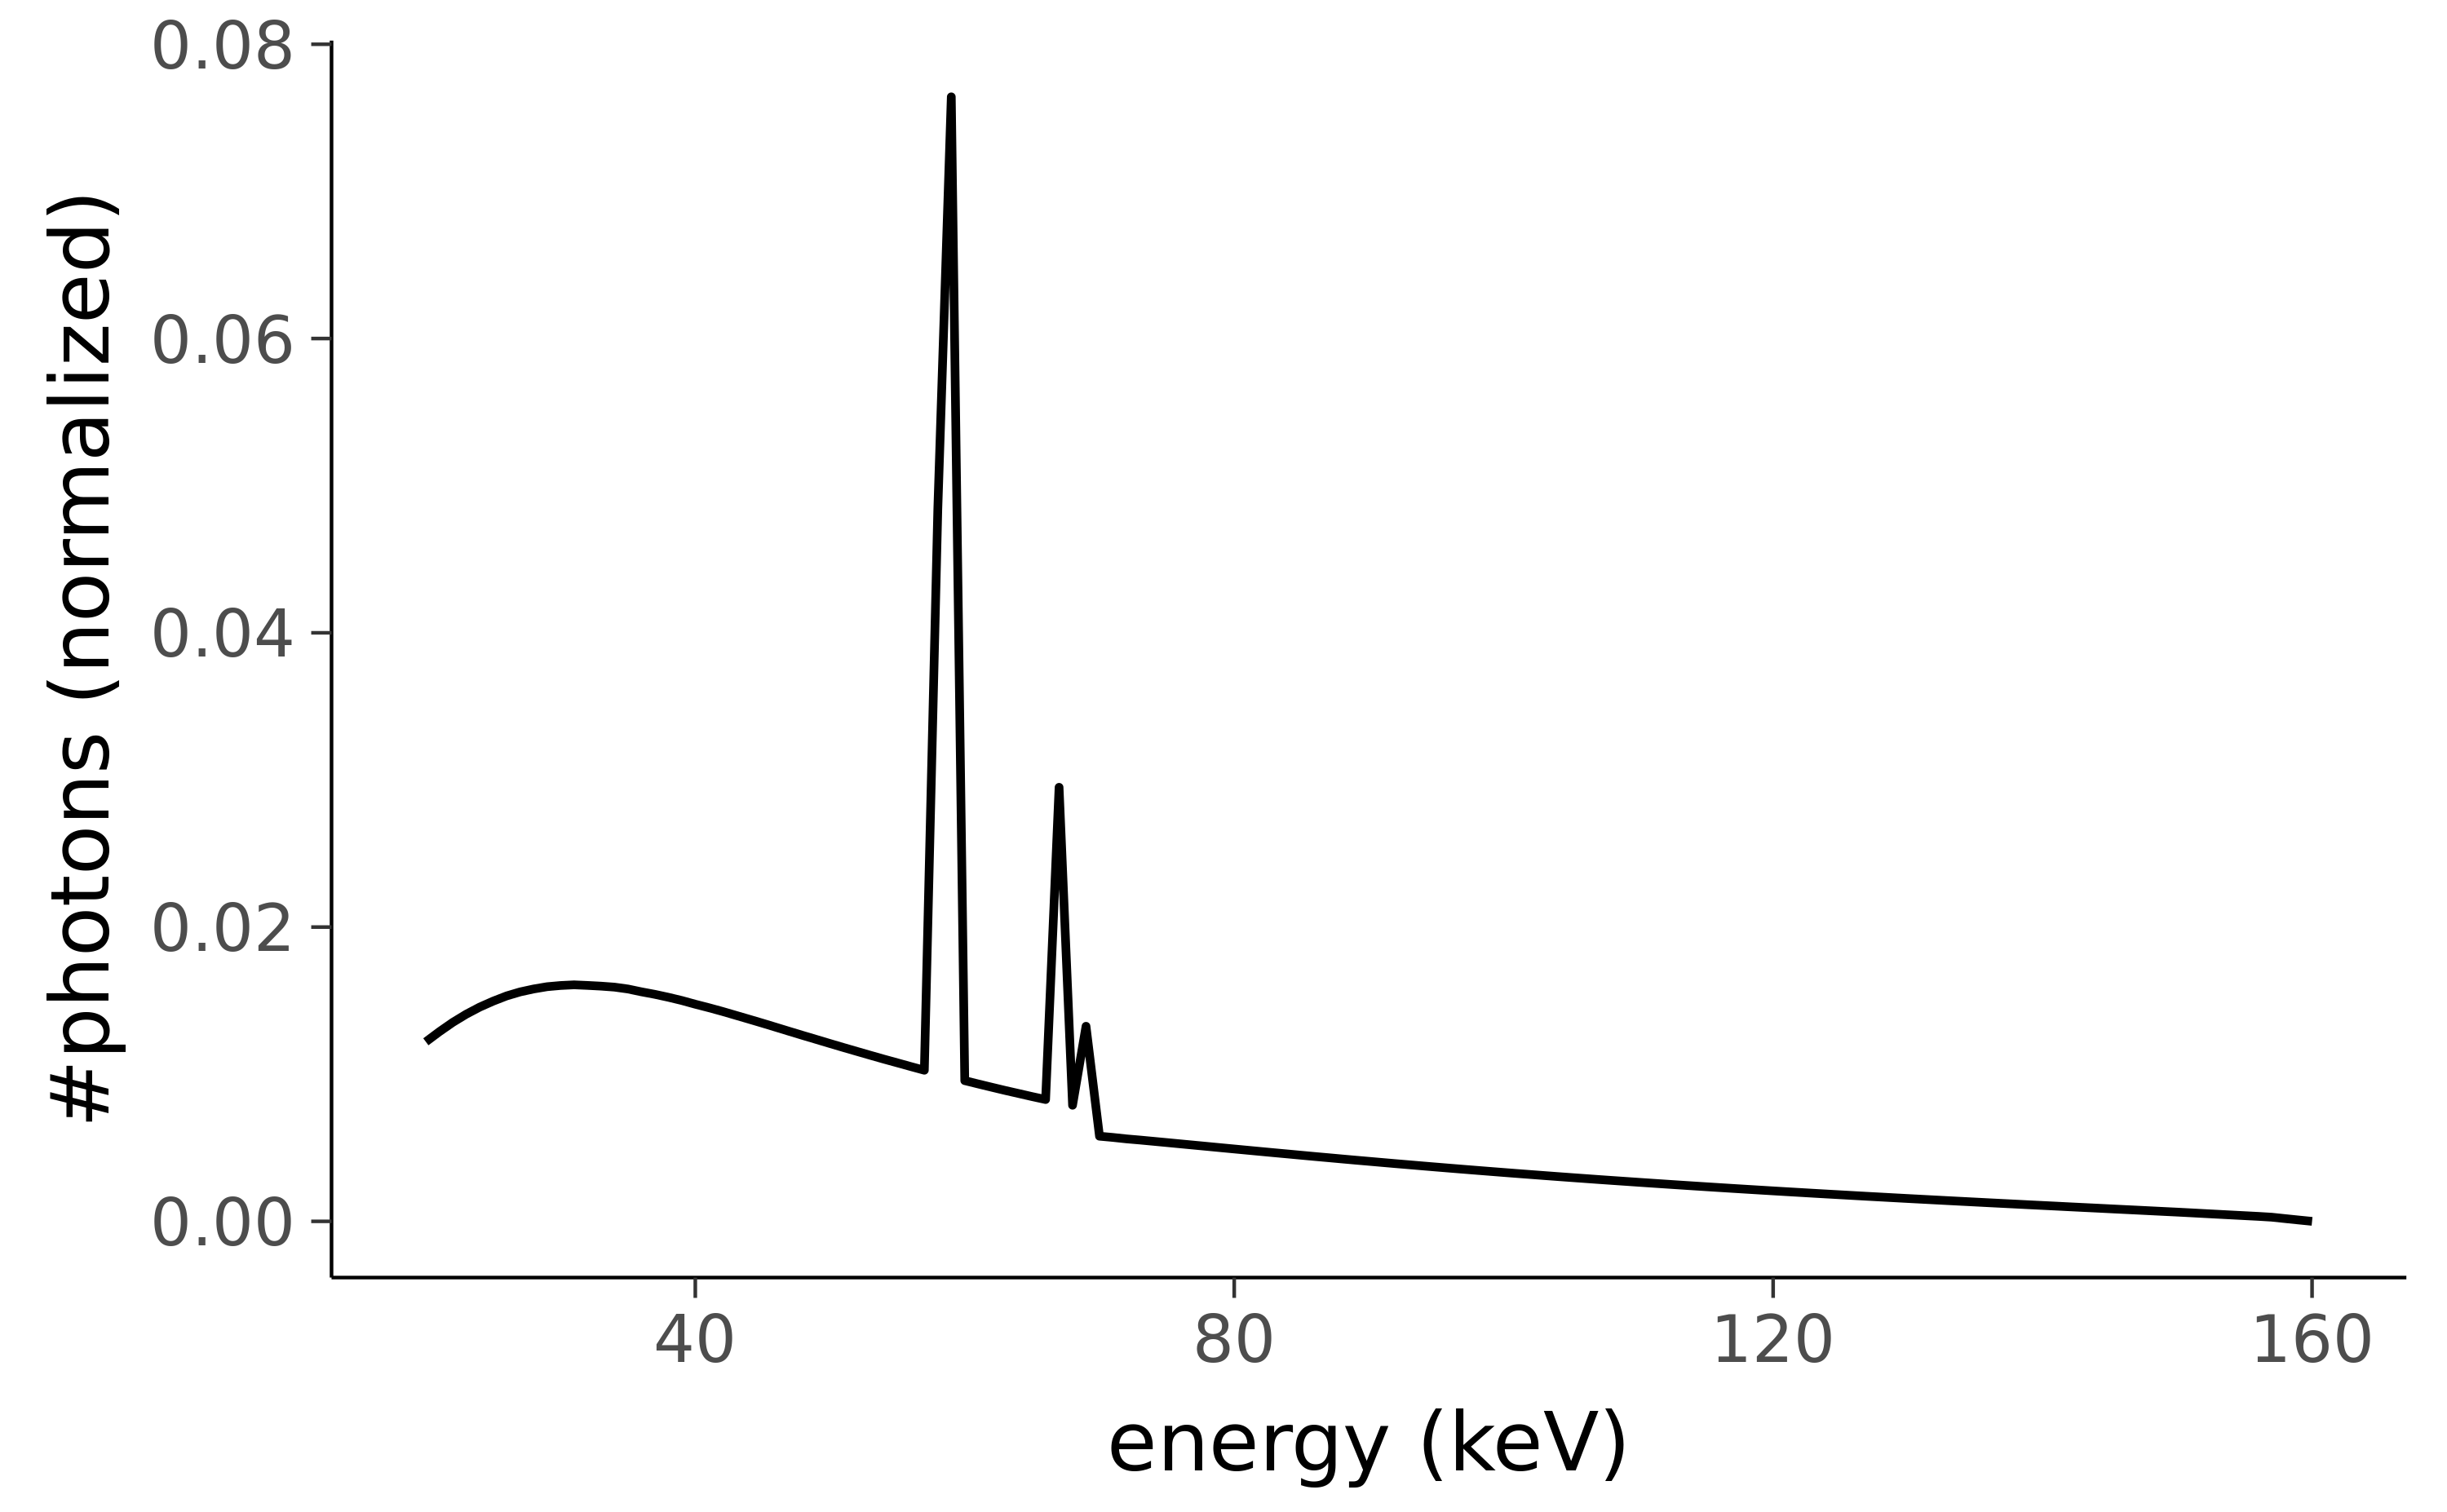
\includegraphics[width=\textwidth]{gfx/spectrum-visibility/spectrum.png}
    \caption{}
    \label{fig:spectrum}
    \end{subfigure}
    \hfill
    \begin{subfigure}[b]{.49\textwidth}
    \centering
    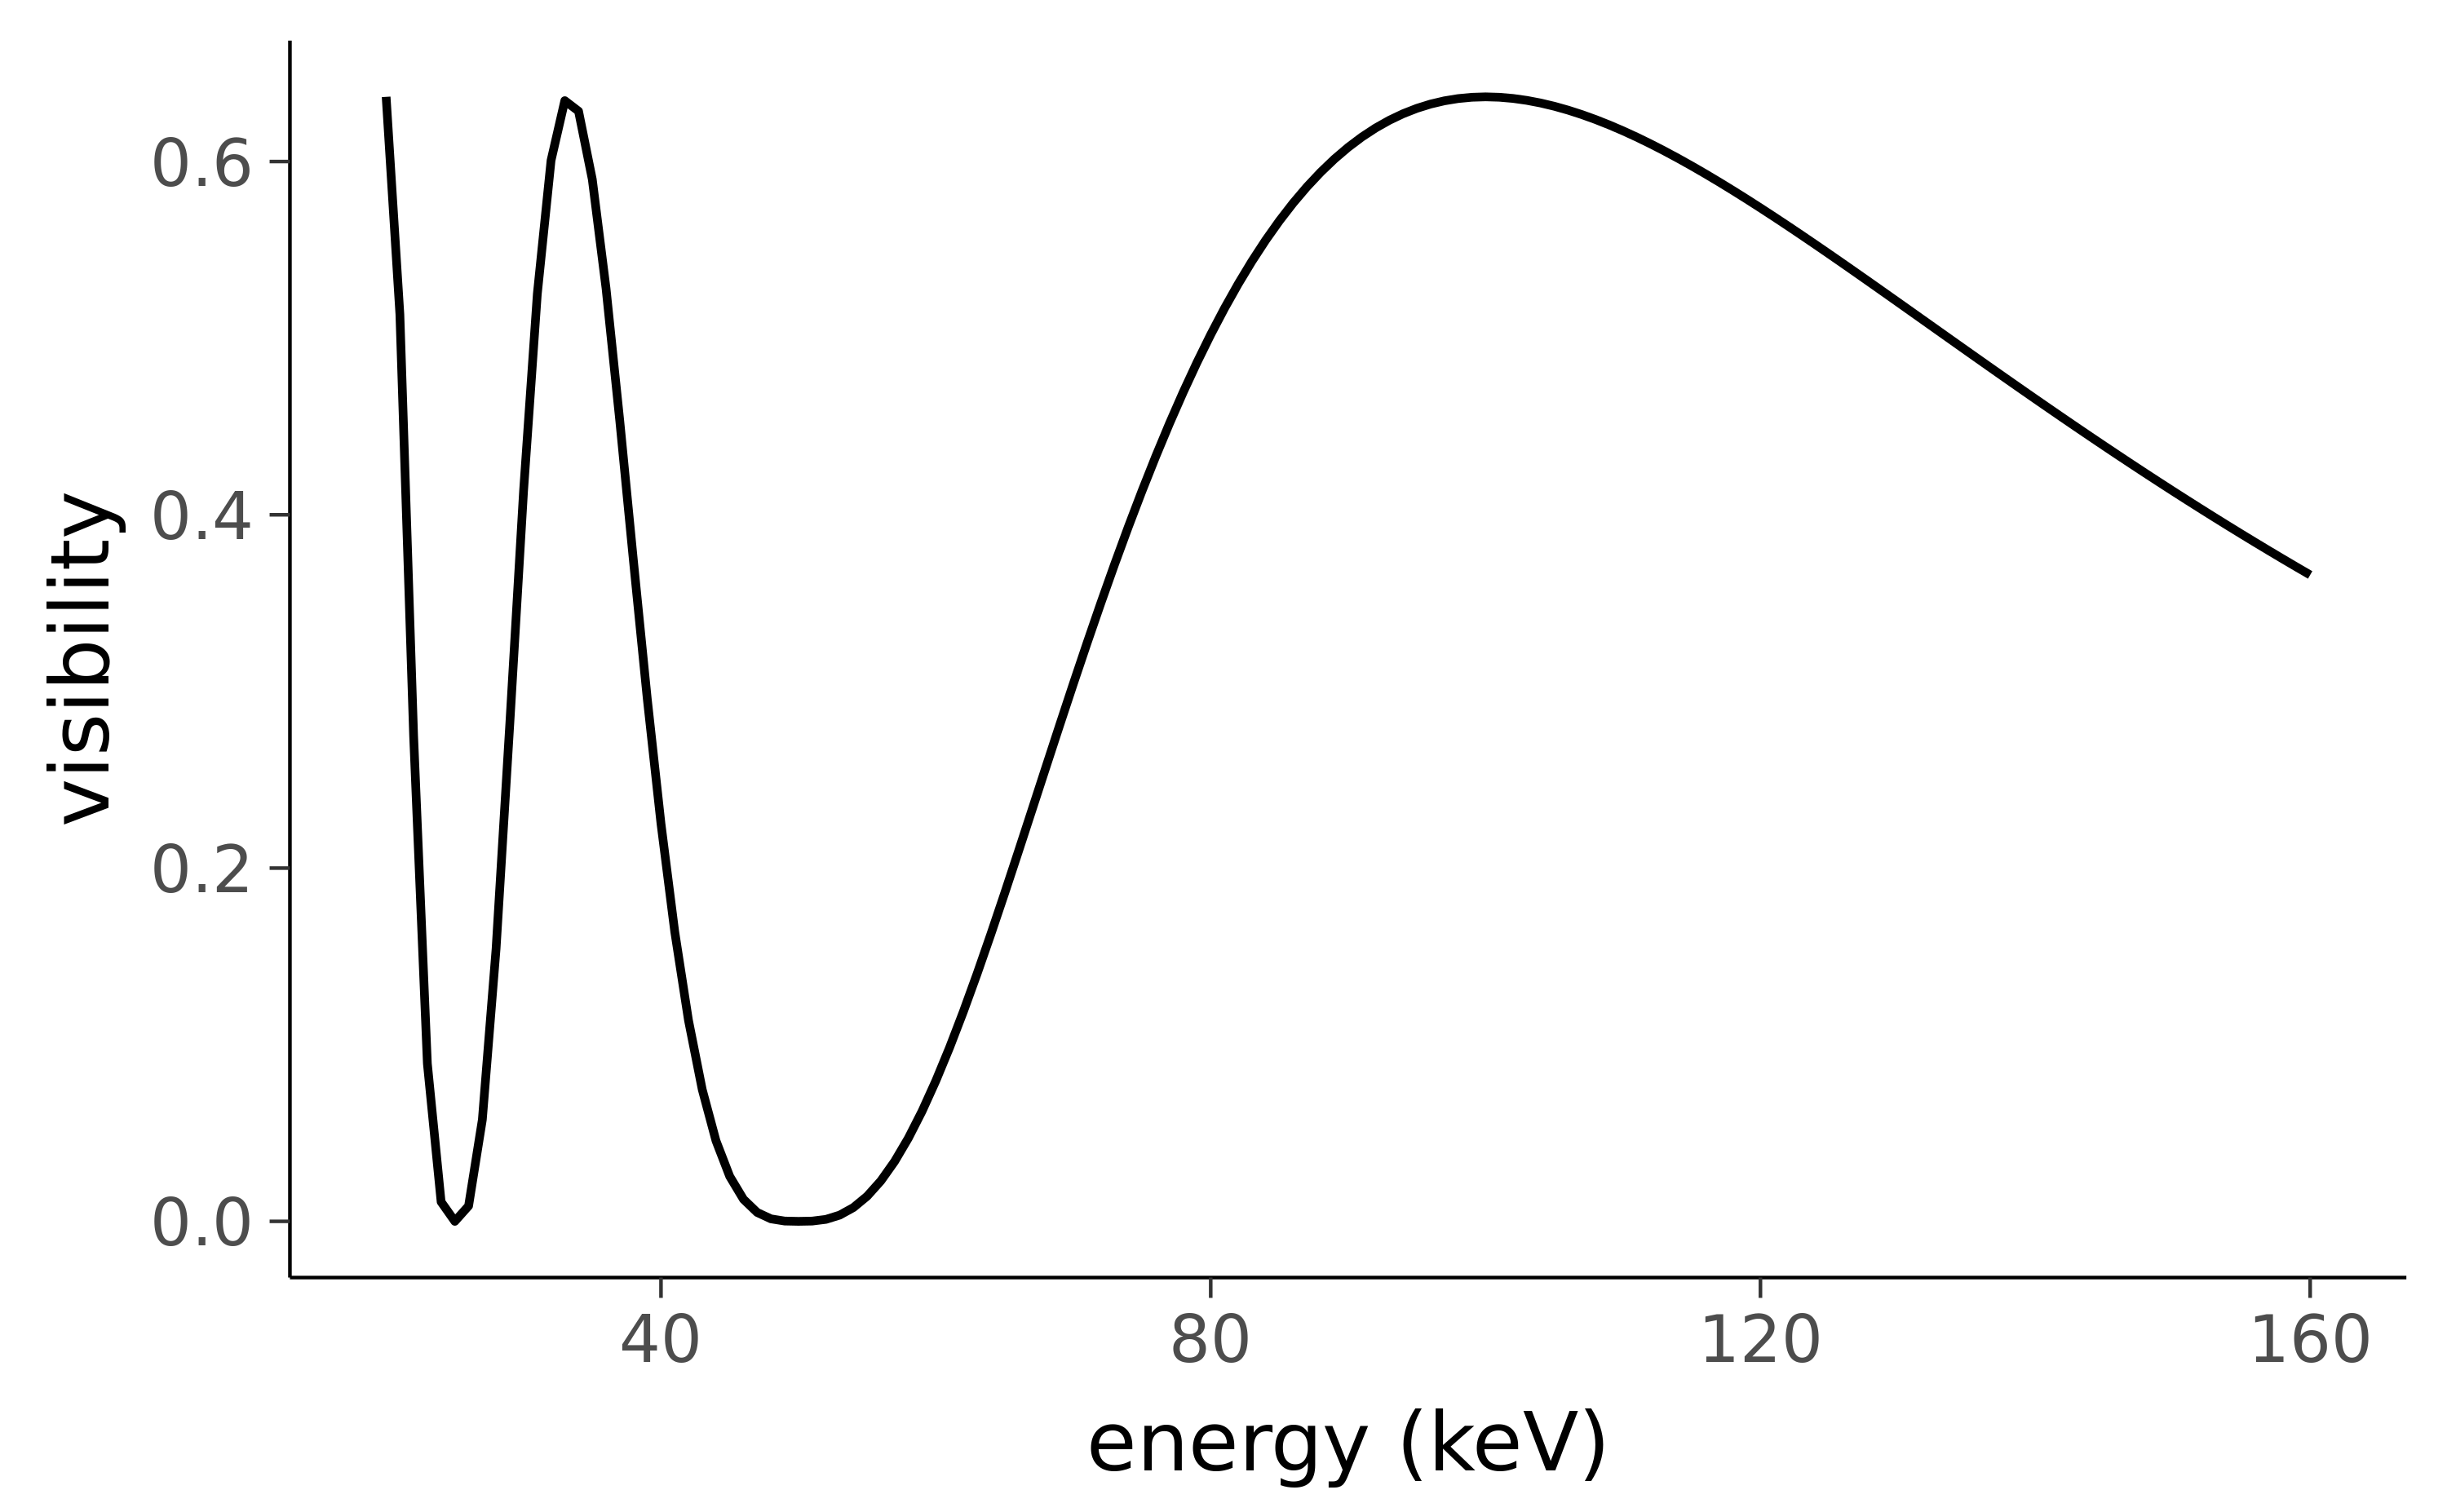
\includegraphics[width=\textwidth]{gfx/spectrum-visibility/visibility.png}
    \caption{}
    \label{fig:visibility}
    \end{subfigure}
    \caption[Spectrum and theoretical visibility of the \SI{100}{\kilo\eV}
    interferometer.]{Spectrum of the source~\ref{fig:spectrum} at \SI{160}{\kilo\voltpeak}
simulated with the SpekCalc software~\cite{spekcalc}. Visibility as a
function of energy for a design energy of \SI{100}{\kilo\eV} at the first
Lohmann distance, calculated according to
equation~\ref{eq:visibility.energy} from~\cite{Thuering20130027}.}
    \label{fig:visibility.energy}
\end{figure}

Running the calculation for our case with the spectral weights $w(\energy)$ shown in
figure~\ref{fig:spectrum} and by summing each contribution to the total
visibility we obtain a theoretical maximum of

\begin{equation}
    v_{theory} = \sum_\energy w(\energy)v(\energy) = 0.26.
    \label{eq:maximum.visibility}
\end{equation}

The achieved values are much lower, around \SI{5}{\percent}, but it is clear
that there is the chance to at least double or triple this value as more
advanced fabrication techniques for the absorption gratings are established.

\section{Results}
We introduce a method for phase contrast imaging which works on
conventional X-ray sources, covers the entire diagnostic X-ray energy range
and is compatible with compact imaging arrangements. 

\begin{figure}[h!]
    \centering
    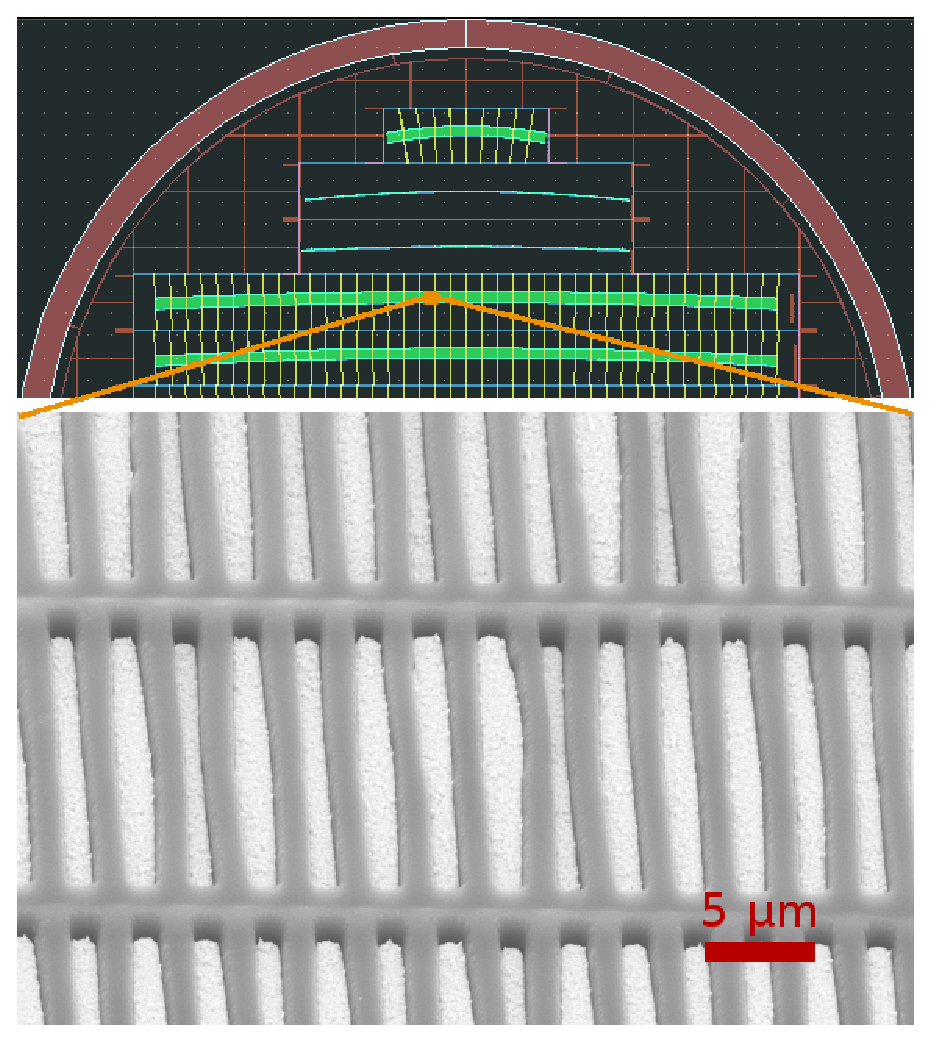
\includegraphics[width=\textwidth]{gfx/grating_mask.eps}
    \caption{Grating design mask for
        the edge-on illumination approach and \ac{SEM}
        image of the grating. The top part of the 4 inch wafer shows
        five grating chips. From top to bottom, one source grating, two
        phase gratings and two analyzer gratings. The
        gratings have different curvatures which are specific to the grating
        interferometer geometry. Multiple gratings for more than one setup
        geometry are fabricated on a single wafer.
        The \ac{SEM} image shows the gold structures and the interrupting bridges
        that prevent the lamellae from collapsing~\cite{Kenntner2010}.}\label{Fig:grating_mask}
\end{figure}

Due to the large spectral acceptance~\cite{Weitkamp2005,Thuering2013c} of the
interferometer ($\SI{50}{\kilo\electronvolt}$ to
more than $\SI{160}{\kilo\electronvolt}$) and the high attenuation efficiencies of
the source and analyzer gratings (more than $90\%$ up to
$\SI{160}{\kilo\electronvolt}$), the voltage of the X-ray source was set to
the maximum of $\SI{160}{\kilo\volt}$. With a structure height of
approximately $\SI{100}{\micro\metre}$, the field of view in the vertical
direction is limited to one detector pixel row. In the horizontal direction,
the field of view is only limited by the grating size to
$\SI{30}{\milli\metre}$, but wider gratings can be fabricated with the same
method and the available technology on larger wafers. In addition to the standard components (source,
camera, interferometer), two optical slits, one in front of the source
grating, the other in front of the camera, were required for the collimation
of the beam in the vertical direction (see figure~\ref{fig:edge.on.photos}). 

\begin{figure}[ht]
    \centering
    \includegraphics[width=.9\textwidth]{gfx/side.png}
    \includegraphics[width=.9\textwidth]{gfx/line.png}
    \caption{Photographs of the edge-on interferometer setup, seen
    from the side and from the source.}\label{fig:edge.on.photos}
\end{figure}

Figure~\ref{fig:img_chip} shows the first X-ray images acquired with our new setup, based on
edge-on illuminated grating interferometry powered by a conventional X-ray
source operated at \SI{160}{\kilo\voltpeak} and with a design energy of
\SI{100}{\kilo\eV}. The sample is an electronic chip, pictured in
figure~\ref{fig:chip_photo}, along with a superposition of the differential
phase X-ray reconstruction.

\begin{figure}[htb]
    \centering
    \begin{subfigure}[b]{.49\textwidth}
    \centering
    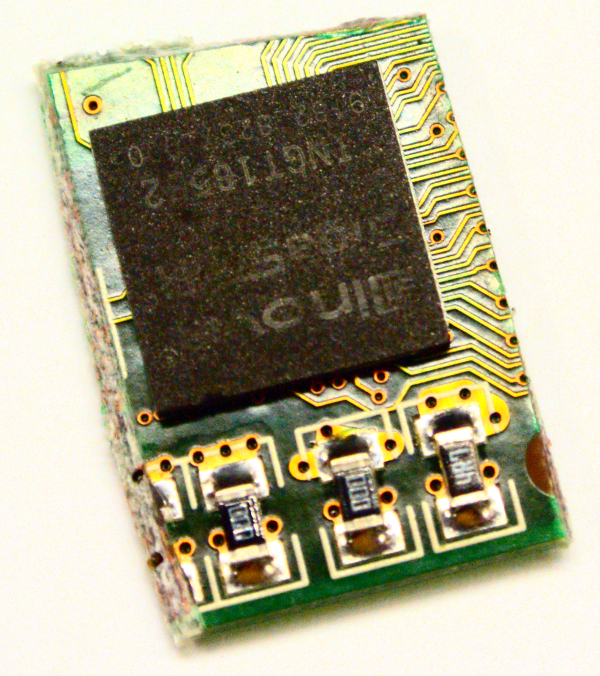
\includegraphics[width=\textwidth]{gfx/mythen-edge-on/chip_overlay_empy.png}
    \caption{}
    \end{subfigure}
    \begin{subfigure}[b]{.49\textwidth}
    \centering
    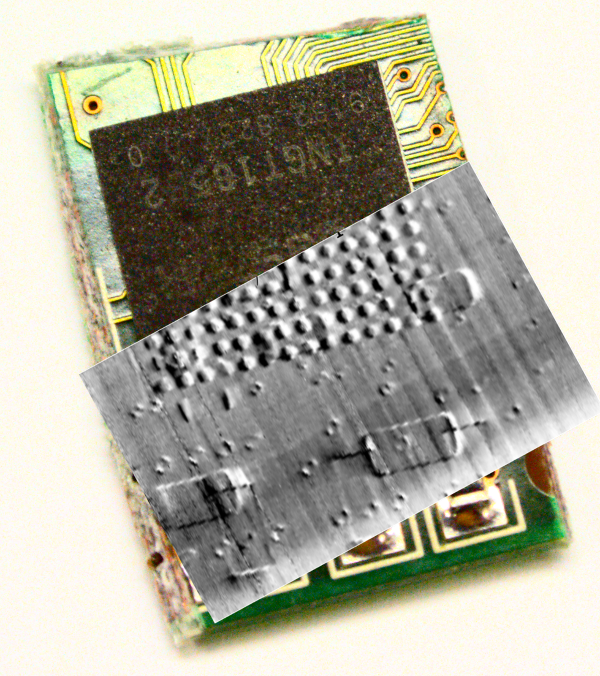
\includegraphics[width=\textwidth]{gfx/mythen-edge-on/chip_overlay_full.png}
    \caption{}
    \end{subfigure}
    \caption{The electronic chip reconstructed in figure~\ref{fig:img_chip},
comparing an optical picture and the reconstructed X-ray differential phase
image.}
    \label{fig:chip_photo}
\end{figure}

\begin{figure}[htp]
    \centering
    %% Creator: Matplotlib, PGF backend
%%
%% To include the figure in your LaTeX document, write
%%   \input{<filename>.pgf}
%%
%% Make sure the required packages are loaded in your preamble
%%   \usepackage{pgf}
%%
%% Figures using additional raster images can only be included by \input if
%% they are in the same directory as the main LaTeX file. For loading figures
%% from other directories you can use the `import` package
%%   \usepackage{import}
%% and then include the figures with
%%   \import{<path to file>}{<filename>.pgf}
%%
%% Matplotlib used the following preamble
%%   \usepackage{fontspec}
%%
\begingroup%
\makeatletter%
\begin{pgfpicture}%
\pgfpathrectangle{\pgfpointorigin}{\pgfqpoint{4.600000in}{7.000000in}}%
\pgfusepath{use as bounding box, clip}%
\begin{pgfscope}%
\pgfsetbuttcap%
\pgfsetmiterjoin%
\definecolor{currentfill}{rgb}{1.000000,1.000000,1.000000}%
\pgfsetfillcolor{currentfill}%
\pgfsetlinewidth{0.000000pt}%
\definecolor{currentstroke}{rgb}{1.000000,1.000000,1.000000}%
\pgfsetstrokecolor{currentstroke}%
\pgfsetdash{}{0pt}%
\pgfpathmoveto{\pgfqpoint{0.000000in}{0.000000in}}%
\pgfpathlineto{\pgfqpoint{4.600000in}{0.000000in}}%
\pgfpathlineto{\pgfqpoint{4.600000in}{7.000000in}}%
\pgfpathlineto{\pgfqpoint{0.000000in}{7.000000in}}%
\pgfpathclose%
\pgfusepath{fill}%
\end{pgfscope}%
\begin{pgfscope}%
\pgfpathrectangle{\pgfqpoint{0.507639in}{4.853494in}}{\pgfqpoint{3.915694in}{1.792145in}}%
\pgfusepath{clip}%
\pgfsys@transformshift{0.507639in}{4.853494in}%
\pgftext[left,bottom]{\pgfimage[interpolate=true,width=3.916667in,height=1.793333in]{images_S00075_S00071-img0.png}}%
\end{pgfscope}%
\begin{pgfscope}%
\pgftext[x=2.465486in,y=6.728972in,,base]{\rmfamily\fontsize{11.000000}{13.200000}\selectfont absorption}%
\end{pgfscope}%
\begin{pgfscope}%
\pgfpathrectangle{\pgfqpoint{0.507639in}{2.636108in}}{\pgfqpoint{3.915694in}{1.792145in}}%
\pgfusepath{clip}%
\pgfsys@transformshift{0.507639in}{2.636108in}%
\pgftext[left,bottom]{\pgfimage[interpolate=true,width=3.916667in,height=1.793333in]{images_S00075_S00071-img1.png}}%
\end{pgfscope}%
\begin{pgfscope}%
\pgftext[x=2.465486in,y=4.511586in,,base]{\rmfamily\fontsize{11.000000}{13.200000}\selectfont differential phase}%
\end{pgfscope}%
\begin{pgfscope}%
\pgfpathrectangle{\pgfqpoint{0.507639in}{0.418722in}}{\pgfqpoint{3.915694in}{1.792145in}}%
\pgfusepath{clip}%
\pgfsys@transformshift{0.507639in}{0.418722in}%
\pgftext[left,bottom]{\pgfimage[interpolate=true,width=3.916667in,height=1.793333in]{images_S00075_S00071-img2.png}}%
\end{pgfscope}%
\begin{pgfscope}%
\pgftext[x=2.465486in,y=2.294200in,,base]{\rmfamily\fontsize{11.000000}{13.200000}\selectfont dark field}%
\end{pgfscope}%
\end{pgfpicture}%
\makeatother%
\endgroup%

    \caption{Radiographic scan of an electronic chip. The image was acquired
        with 24 phase steps per line and an exposure time of \SI{15}{\second} per
    step. The top right image shows the differential absorption image.}\label{fig:img_chip}
\end{figure}

Several resistors and integrated circuits located on different
layers on an electronic chip can be identified. The radiographs were acquired in scanning
mode, using a step size of \SI{100}{\micro\metre} along the $y$ axis, covering a total imaging
area of $2 \times \SI{2}{\centi\metre^2}$. For a better comparison of the magnified phase and
attenuation images, the latter has been replaced with the differential
attenuation image, which was obtained by calculating the derivative along
the horizontal axis. In the attenuation image, the contrast of the soldering
points of the integrated circuit is reduced underneath the resistors, while
in the phase image, they can clearly be identified. The reduced contrast of
the soldering points in the absorption image is due to beam hardening. The
spectrum impinging on these soldering point is hardened by the resistors in
the upper layer, resulting in lower absorption contrast. Due to the weaker
energy dependence of phase shifts ($1/\energy$ compared to $1/\energy^3$), phase-contrast
images are less sensitive to beam hardening~\cite{Chabior2011a}, which explains the lower
contrast reduction of the soldering points under the resistors in the
phase image of the chip. This example shows one of the potential benefits of
phase contrast X-ray imaging at high energies, which may be useful to
identify flaws in multilayered structures such as electronic chips.

Figure~\ref{fig:screw} shows a scan with \num{100} lines over
\SI{1}{\centi\metre} of a zinc screw
with \num{24} phase steps and \SI{15}{\second} exposure time.
The edge-enhancement effects of the differential phase signal are
particularly visible at the edges, where the
derivative~\eqref{eq:refraction.angle} is a maximum.

\begin{figure}[hbt]
    \centering
    %% Creator: Matplotlib, PGF backend
%%
%% To include the figure in your LaTeX document, write
%%   \input{<filename>.pgf}
%%
%% Make sure the required packages are loaded in your preamble
%%   \usepackage{pgf}
%%
%% Figures using additional raster images can only be included by \input if
%% they are in the same directory as the main LaTeX file. For loading figures
%% from other directories you can use the `import` package
%%   \usepackage{import}
%% and then include the figures with
%%   \import{<path to file>}{<filename>.pgf}
%%
%% Matplotlib used the following preamble
%%   \usepackage{fontspec}
%%
\begingroup%
\makeatletter%
\begin{pgfpicture}%
\pgfpathrectangle{\pgfpointorigin}{\pgfqpoint{4.600000in}{6.000000in}}%
\pgfusepath{use as bounding box, clip}%
\begin{pgfscope}%
\pgfsetbuttcap%
\pgfsetmiterjoin%
\definecolor{currentfill}{rgb}{1.000000,1.000000,1.000000}%
\pgfsetfillcolor{currentfill}%
\pgfsetlinewidth{0.000000pt}%
\definecolor{currentstroke}{rgb}{1.000000,1.000000,1.000000}%
\pgfsetstrokecolor{currentstroke}%
\pgfsetdash{}{0pt}%
\pgfpathmoveto{\pgfqpoint{0.000000in}{0.000000in}}%
\pgfpathlineto{\pgfqpoint{4.600000in}{0.000000in}}%
\pgfpathlineto{\pgfqpoint{4.600000in}{6.000000in}}%
\pgfpathlineto{\pgfqpoint{0.000000in}{6.000000in}}%
\pgfpathclose%
\pgfusepath{fill}%
\end{pgfscope}%
\begin{pgfscope}%
\pgfpathrectangle{\pgfqpoint{0.507639in}{3.785028in}}{\pgfqpoint{3.915694in}{1.860611in}}%
\pgfusepath{clip}%
\pgfsys@transformshift{0.507639in}{3.785028in}%
\pgftext[left,bottom]{\pgfimage[interpolate=true,width=3.916667in,height=1.863333in]{images_S00052-img0.png}}%
\end{pgfscope}%
\begin{pgfscope}%
\pgftext[x=2.465486in,y=5.728972in,,base]{\rmfamily\fontsize{11.000000}{13.200000}\selectfont absorption}%
\end{pgfscope}%
\begin{pgfscope}%
\pgfpathrectangle{\pgfqpoint{0.507639in}{2.509834in}}{\pgfqpoint{3.915694in}{0.790970in}}%
\pgfusepath{clip}%
\pgfsys@transformshift{0.507639in}{2.509834in}%
\pgftext[left,bottom]{\pgfimage[interpolate=true,width=3.916667in,height=0.793333in]{images_S00052-img1.png}}%
\end{pgfscope}%
\begin{pgfscope}%
\pgftext[x=2.465486in,y=3.384138in,,base]{\rmfamily\fontsize{11.000000}{13.200000}\selectfont differential phase}%
\end{pgfscope}%
\begin{pgfscope}%
\pgfpathrectangle{\pgfqpoint{0.507639in}{0.699820in}}{\pgfqpoint{3.915694in}{0.790970in}}%
\pgfusepath{clip}%
\pgfsys@transformshift{0.507639in}{0.699820in}%
\pgftext[left,bottom]{\pgfimage[interpolate=true,width=3.916667in,height=0.793333in]{images_S00052-img2.png}}%
\end{pgfscope}%
\begin{pgfscope}%
\pgftext[x=2.465486in,y=1.574124in,,base]{\rmfamily\fontsize{11.000000}{13.200000}\selectfont dark field}%
\end{pgfscope}%
\end{pgfpicture}%
\makeatother%
\endgroup%

    \caption[Radiography of a zinc screw.]{Radiography of a zinc screw.
        Vertical scan of \SI{1}{\centi\metre} with \num{100} lines,
        \num{24} phase steps $\times$ \SI{15}{\second} exposure time.}
    \label{fig:screw}
\end{figure}

\section{Discussion}
Possible usages of edge-on grating interferometry encompass applications
ranging from medical imaging to non-destructive testing and homeland
security. All these applications seek for high (greater than
\SI{100}{\kilo\eV}) nominal energies
and compact designs. Particularly for medical application, the operation of
a phase contrast imaging device at high energies is imperative. When imaging
patients, a crucial issue is the dose, which depends mainly on the
absorption of the X-rays and decreases with the third power of the photon
energy~\cite{Momose2005}. On the other hand, the phase interaction is only inversely
proportional to the energy and is therefore relatively much more relevant
than absorption as the energy increases, possibly leading to a decreased
exposure for an equivalent image quality. Clinical operation of such a
device will imply measuring patients who normally breath, move and shake.
Fast acquisitions are therefore required, in order to keep the images sharp
and artifact free. As a consequence, compact, efficient imaging systems need
to be developed to provide imaging capabilities at sufficient speed. Our
circular grating alignment matches the structures of the diffracting and
absorbing elements to the divergent beam, especially for compact geometries.
In conclusion, short, high-energy phase-contrast systems will enable the
efficient investigation of high-density materials or thick samples, adding
information on electron density and integrated small-angle scattering power
to the conventional absorption-based signal. This will improve material
discrimination and density sensitivity in future X-ray or even
neutron~\cite{Grunzweig2008} investigations.

\section{Methods}
Edge-on illuminated gratings were manufactured by Microworks GmbH, Germany, using a LIGA process~\cite{Kenntner2010}. Each grating
resides on a $5 \times \SI{60}{\milli\metre^2}$ silicon chip and several
grating chips are fabricated on a single 4 inch silicon wafer. The
experimental arrangement for a design energy at \SI{100}{\kilo\electronvolt}
is a symmetric Talbot-Lau interferometer with a grating period of $p =
\SI{2.8}{\micro \metre}$ for all gratings. The distance from the source
grating to the analyzer grating is $\SI{32}{\centi\metre}$ and the source
grating is positioned $\SI{23}{\centi\metre}$ away from the source.

The X-ray source is a tungsten target COMET MXR-160HP/11 X-ray tube with a maximum output
voltage of $\SI{160}{\kilo\volt}$ and a current of $\SI{10}{\milli\ampere}$. In the experiment, it was set to the
maximum voltage. The focal spot size is approximately
$\SI{1}{\milli\metre}$. The detector is a CCD camera from Finger Lakes
Instruments. A cesium iodide (CsI:Tl) scintillator of $\SI{600}{\micro
\metre}$ thickness converts the X-rays to visible light and is coupled to
an optical lens projecting the image onto the CCD\@. The effective pixel size
is $\SI{80}{\micro\metre}$. The collimating slit right after the source is 
$\SI{25}{\micro\metre}$ wide, while the second slit before the detector is
$\SI{100}{\micro\metre}$.

In figure~\ref{fig:img_chip}, image acquisition involved 24 phase steps per
line and an exposure time of 15 seconds per step. The long
exposure times are mostly constrained by the low average visibility of the
gratings (\SI{5}{\percent}). The exposure time was chosen in order to
get a low noise in the differential phase image. The \ac{SNR} is
proportional to the visibility and the square root of the exposure
time~\cite{Raupach2011}.
This implies that the exposure times can easily drop by an order of
magnitude as these gratings become comparable in quality to those developed
in the last ten years. 
Smaller regions of these gratings already exhibit a visibility up
to~\SI{14}{\percent}, indicating that this goal is reachable as the
fabrication becomes more reliable and uniform.

\section{Towards quantitative evaluations}
In the previous sections, the results providing the \emph{first light}
through Talbot-Lau interferometers at \SI{160}{\kilo\voltpeak} have been
shown (figures~\ref{fig:img_chip} and~\ref{fig:screw}). It would therefore
be appropriate to test if the quantitative studies on the differential phase
and dark field signals could be replicated and extended to these setups.

A number of studies have been published over the last few years\cn
connecting the intensity of the recorded dark-field signal to physical
properties of a sample, most notably its structure and its composition. A
preliminary study to determine if such a goal would be attainable in the
edge-on and high-energy configuration has been designed.

This consists of the interferometer with a design energy of
\SI{120}{\kilo\eV} (see table~\ref{tab:gratings}) with a specially modified
detector from the detector group of the Paul Scherrer Institute. The
module is a strip detector with 1280 photon counting channels, arranged to
match the fan beam curvature at a distance of \SI{70}{\centi\meter} from the
source. The strips are also designed to lie on the beam plane as to achieve
a maximum efficiency as the full \SI{2}{\centi\meter} thickness of silicon
is used to detect the incoming photons (see
figure~\ref{fig:mythen-edge-on}). The resolution of the detector is
\SI{50}{\micro\meter}.

\begin{figure}[htb]
    \centering
    \begin{subfigure}[b]{.49\textwidth}
    \centering
    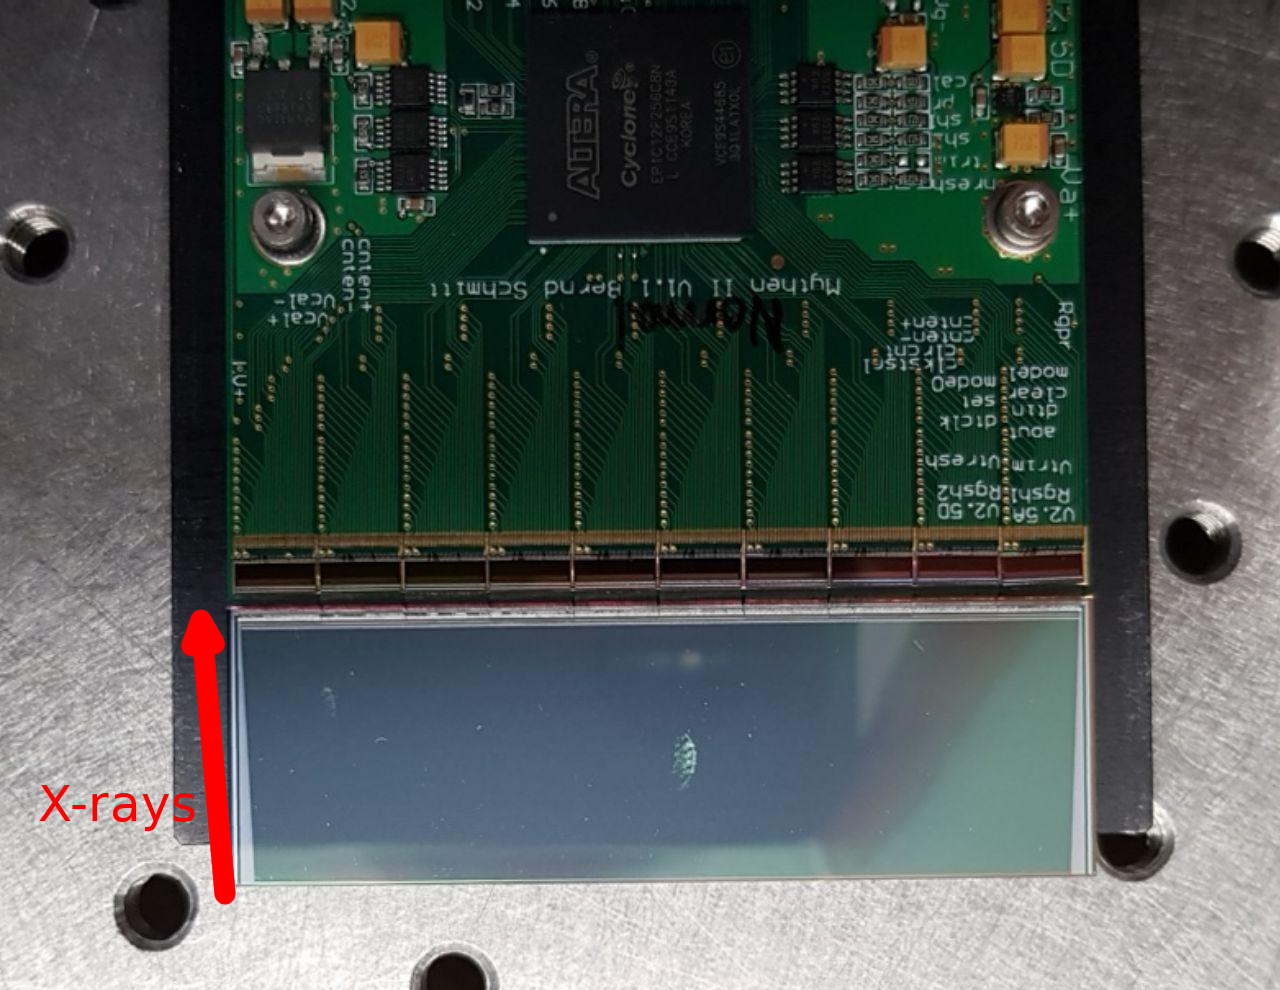
\includegraphics[width=\textwidth]{gfx/mythen-edge-on/mythen.png}
    \caption{}
    \end{subfigure}
    \begin{subfigure}[b]{.49\textwidth}
    \centering
    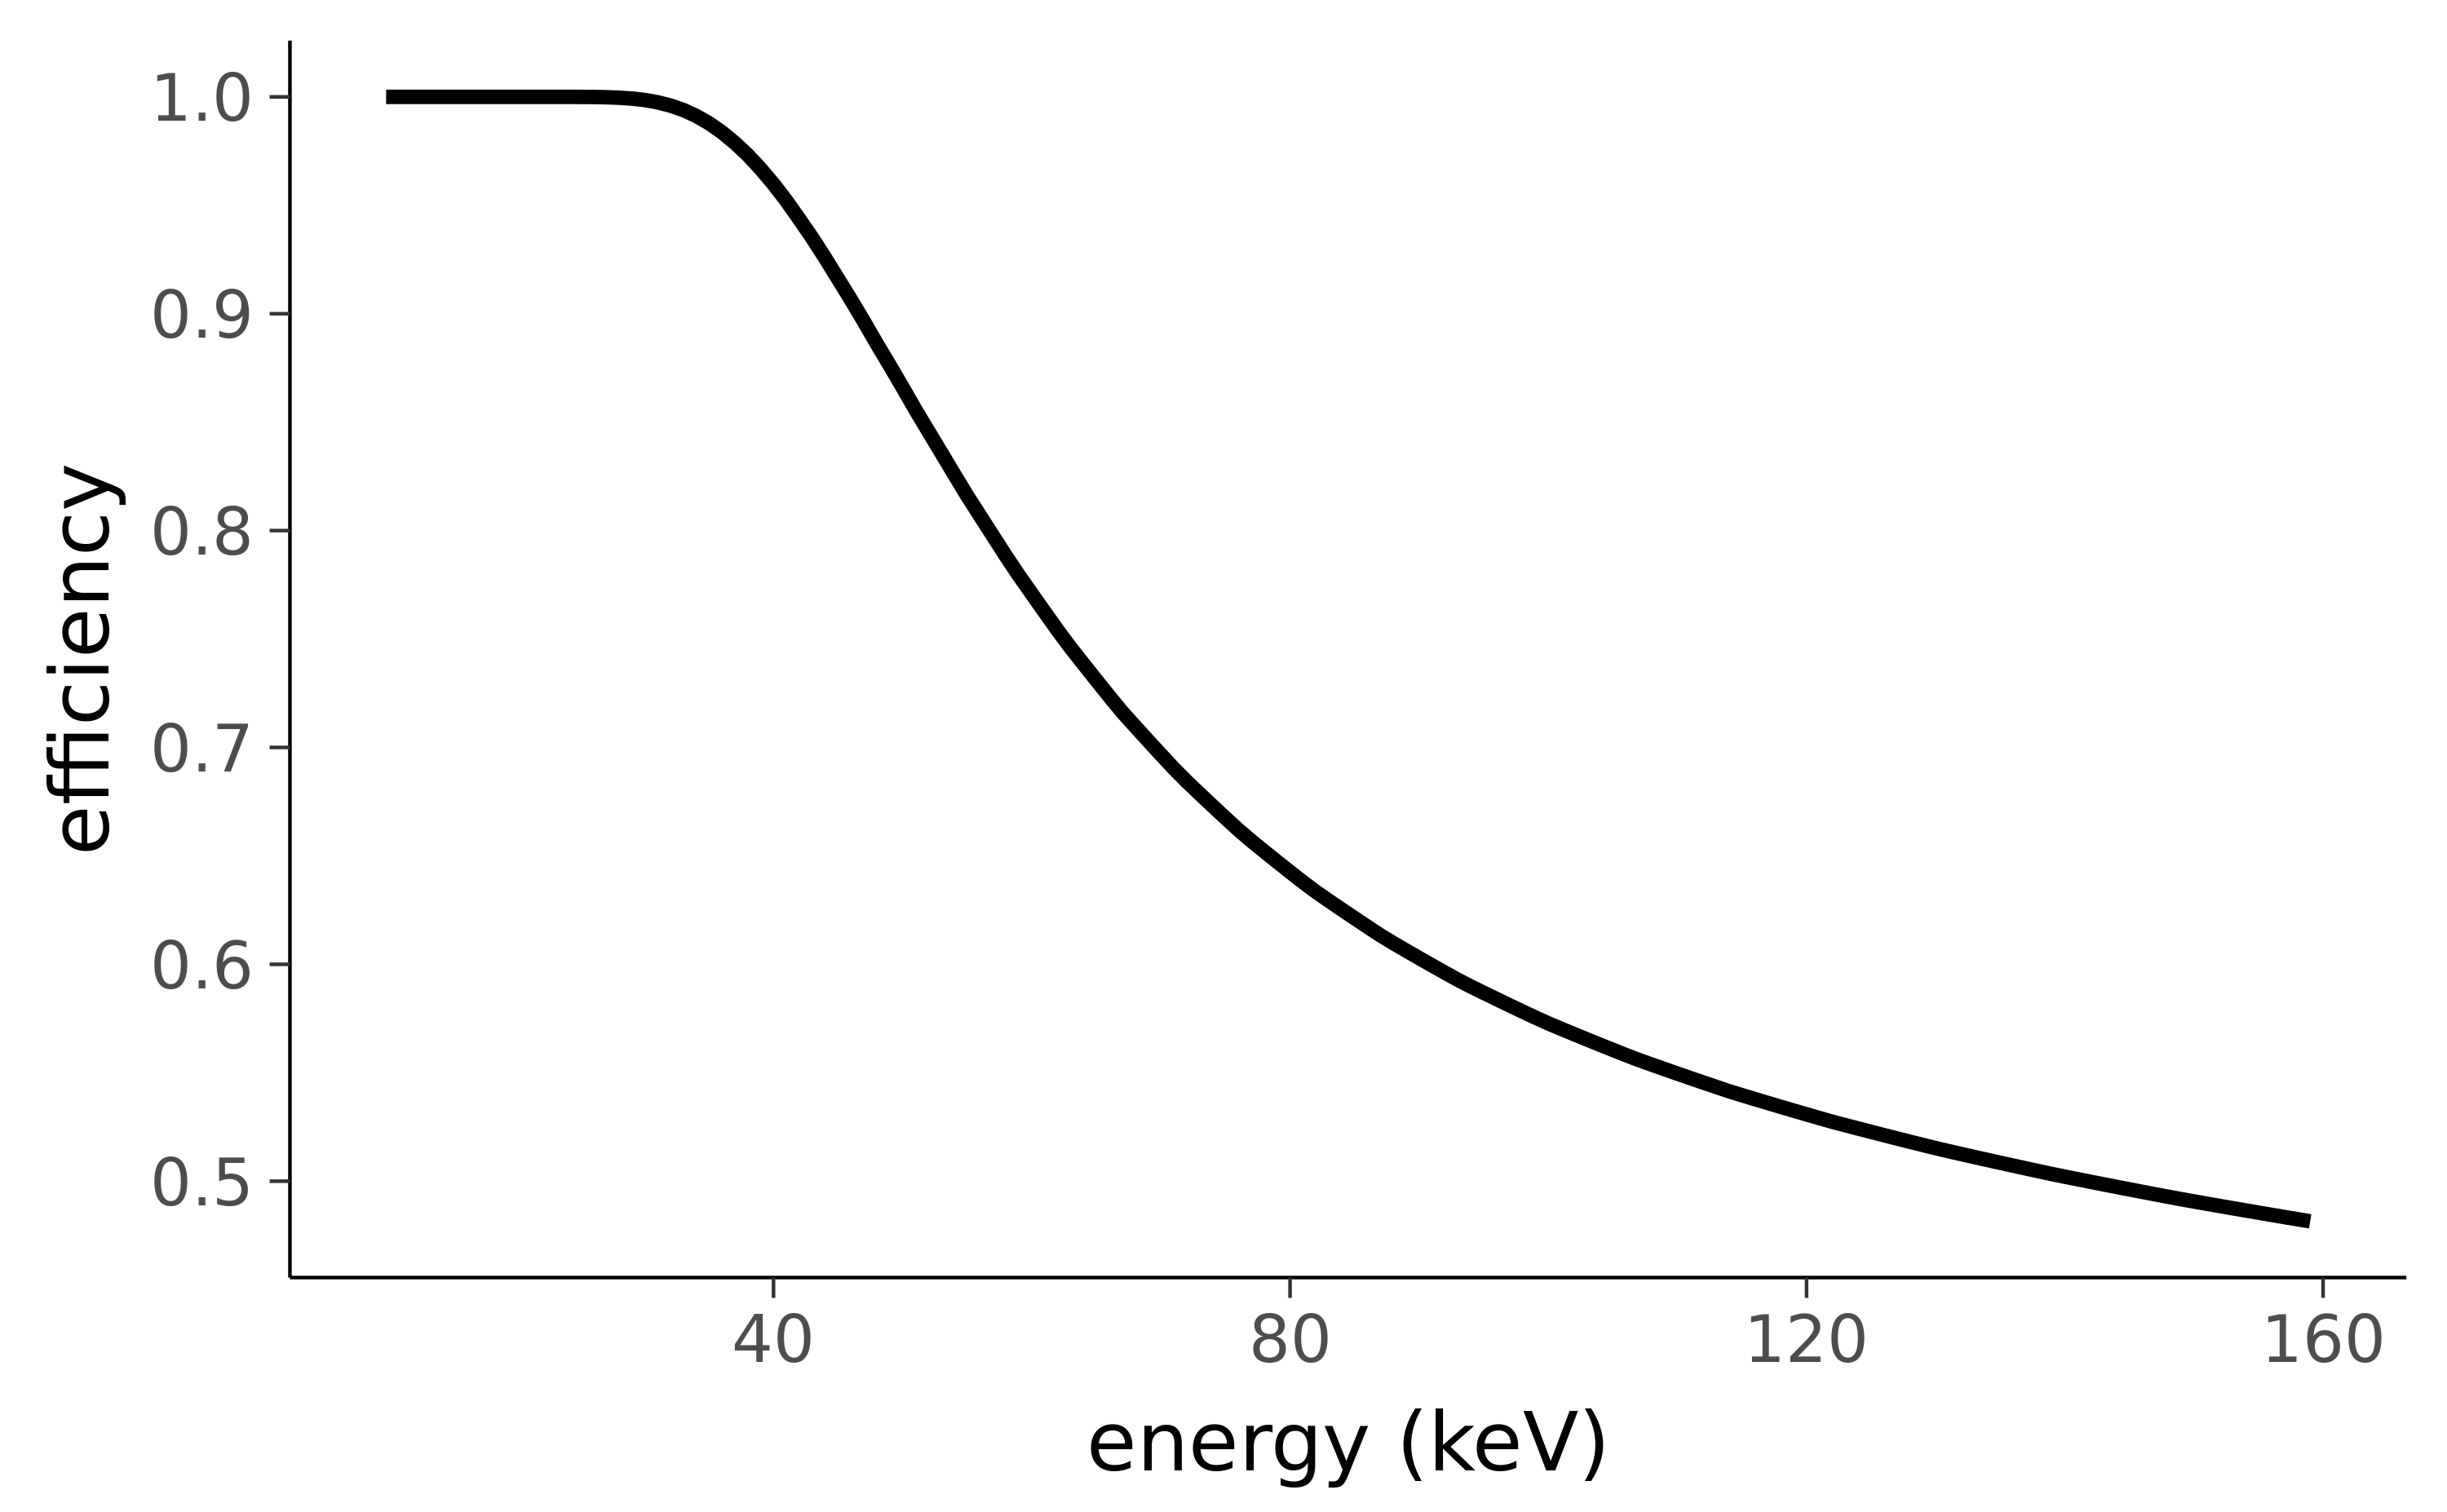
\includegraphics[width=\textwidth]{gfx/mythen-edge-on/efficiency.png}
    \caption{}
    \end{subfigure}
    \caption{A Mythen detector module\cn{mythen} with \SI{2}{\centi\meter} silicon
strips arranged to match a curved fan beam in the edge-on configuration.
This large thickness allows to reach a very high efficiency for a silicon
sensor, without compromising the resolution. The calculated efficiency is above
\SI{50}{\percent} up to \SI{160}{\kilo\eV}.}
    \label{fig:mythen-edge-on}
\end{figure}

The new, custom made, detector matching the circular wave front provides a
significant benefit for the visibility of the interference fringes, which is
improved to an average of \SI{7.5}{\percent}, as shown in
figure~\ref{fig:mythen-visibility}.

\begin{figure}[htb]
    \centering
    \begin{subfigure}[b]{.49\textwidth}
    \centering
    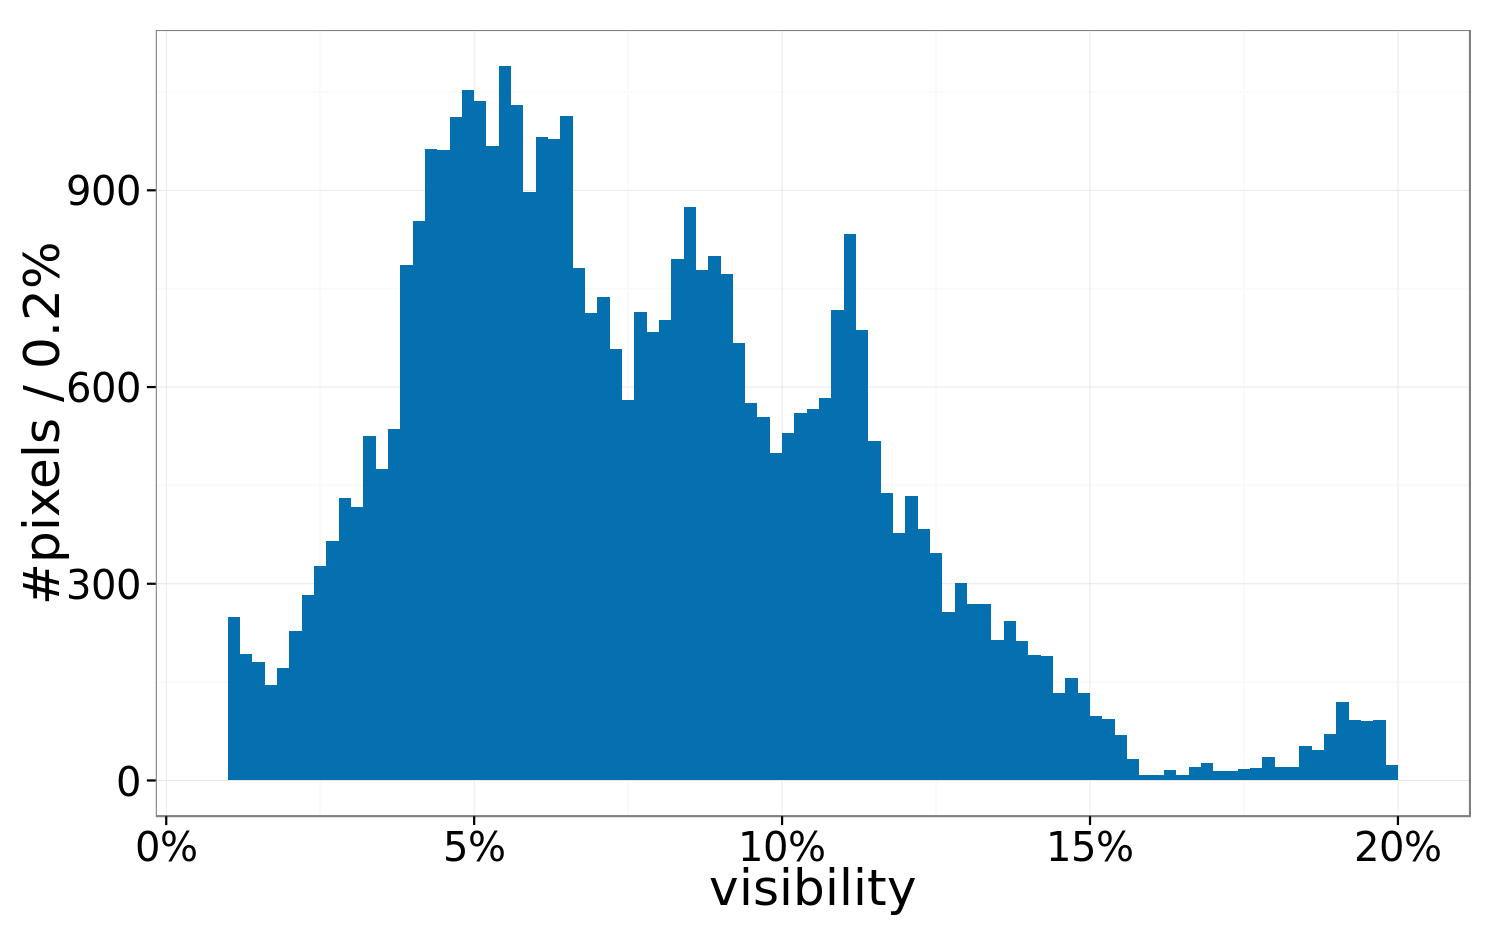
\includegraphics[width=\textwidth]{gfx/mythen-edge-on/visibility.png}
    \caption{}
    \label{fig:mythen-visibility}
    \end{subfigure}
    \hfill
    \begin{subfigure}[b]{.49\textwidth}
    \centering
    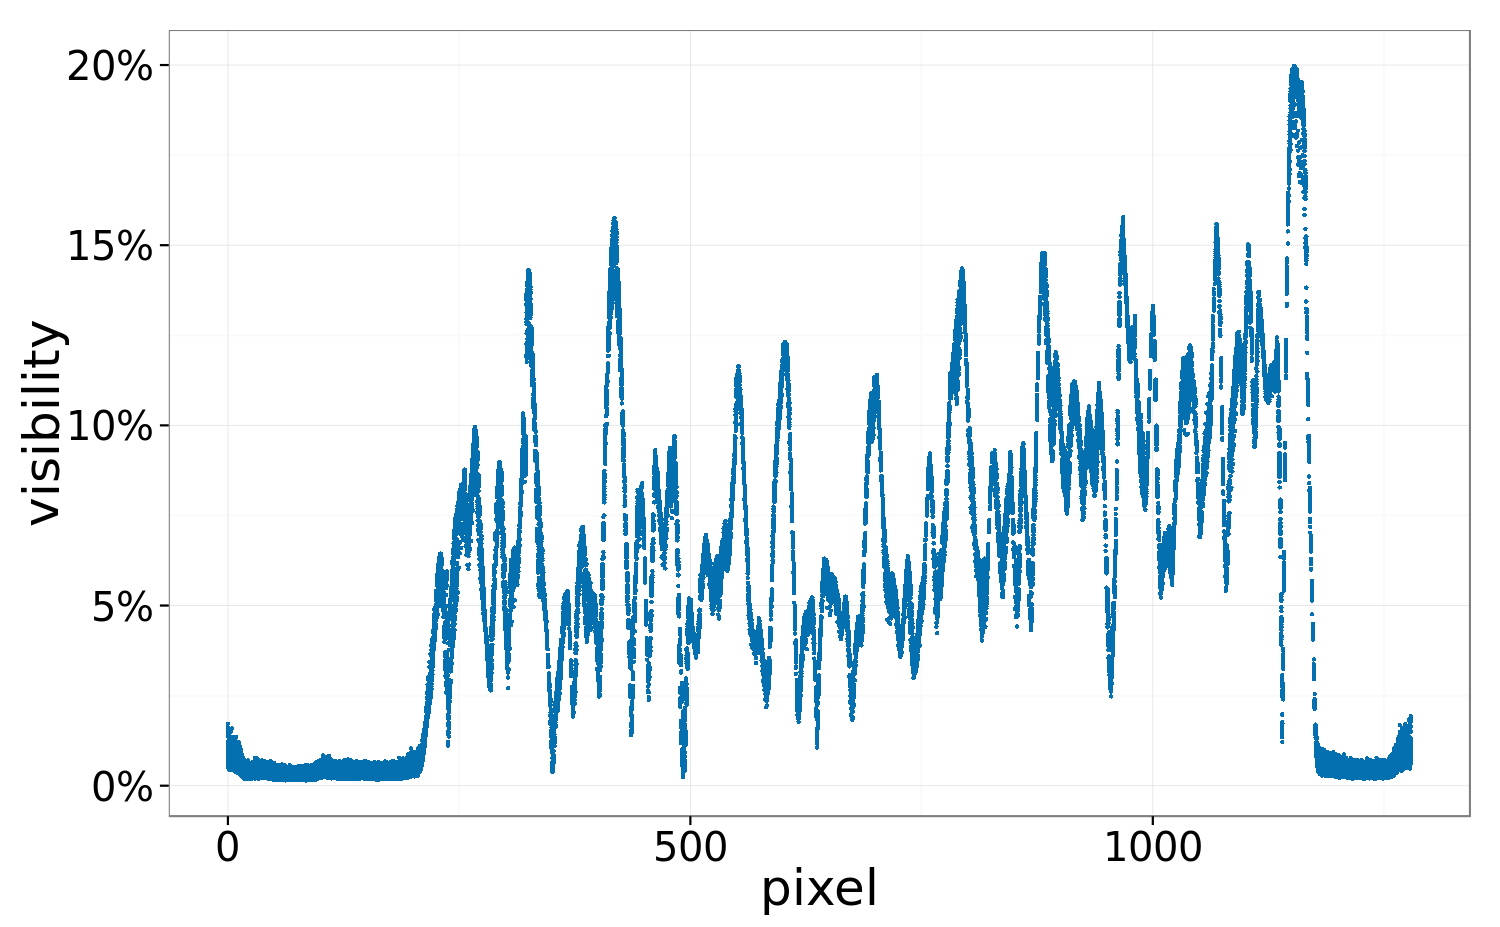
\includegraphics[width=\textwidth]{gfx/mythen-edge-on/pixel_visibility.png}
    \caption{}
    \label{fig:mythen-visibility-pixel}
    \end{subfigure}
    \caption[Visibility of the edge-on grating interferometer with a custom
    detector.]{Visibility histogram and visibility as a function of pixel
        number for the \SI{120}{\kilo\eV} design-energy interferometer with
        a custom silicon sensor matching the wave front curvature attached
        to a Mythen module\cn.
    }
\end{figure}

\subsection{Testing phase sensitivity}
A quantitative test of the differential phase signal can be performed by
using samples in a shape of a wedge with an an angle $\theta$. Such a sample
introduces a constant deviation in the X-ray beam that can be measured and
then averaged across the whole field of view
(figure~\ref{fig:wedge.deviation}).

\begin{figure}[htb]
    \centering
    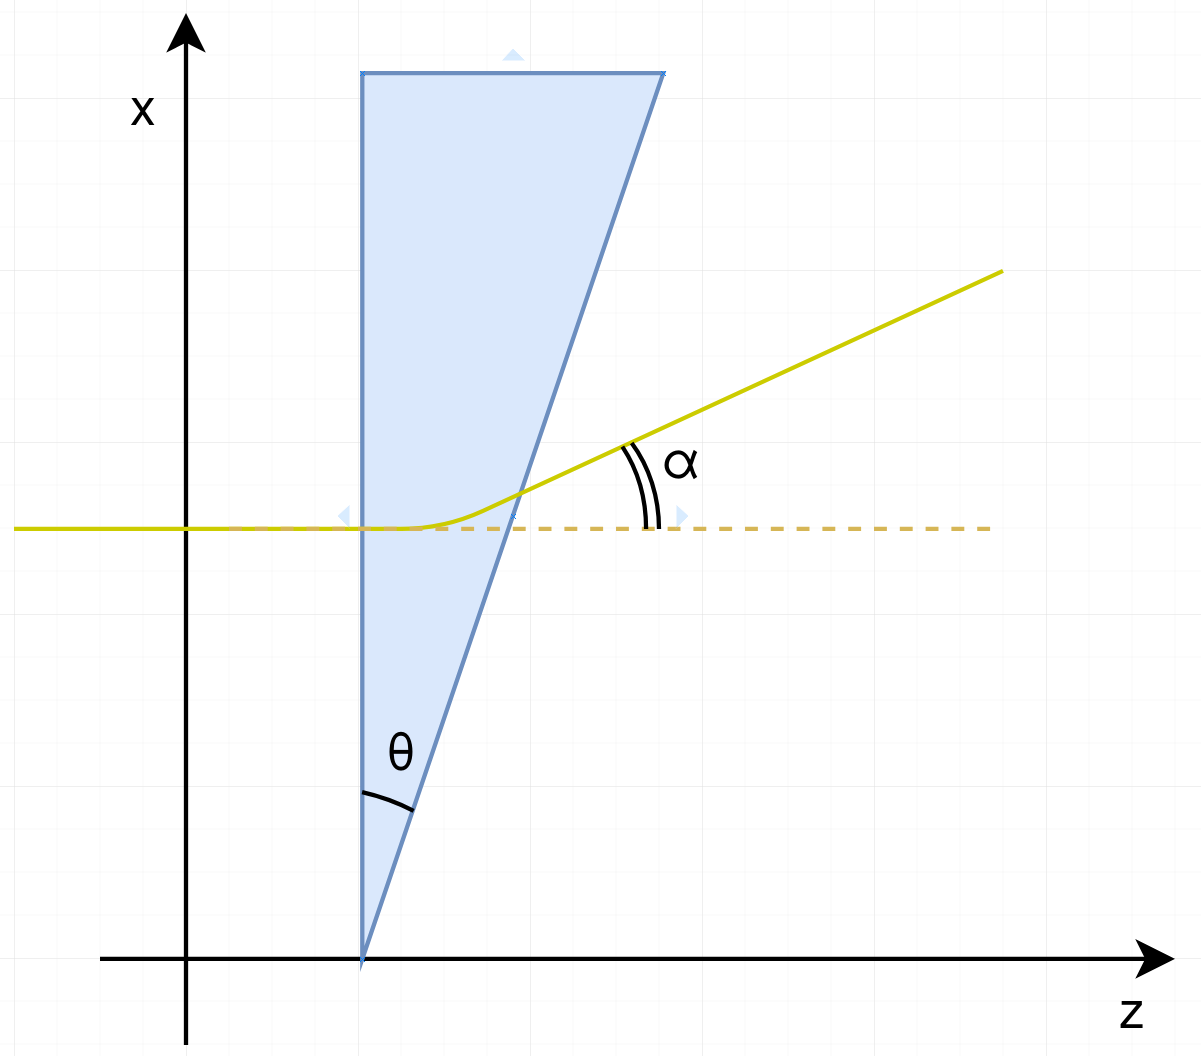
\includegraphics[width=.5\textwidth]{gfx/wedge-deviation.png}
    \caption{Deviation of X-rays introduced by a wedge sample with an angle
    $\theta$.}
    \label{fig:wedge.deviation}
\end{figure}

According to equation~\eqref{eq:phase.deviation}, a thickness $z$ of a
homogeneous material with refractive index $\delta$ introduces a change in
the phase of the X-ray beam according to $\phi = -k\delta z$. In the wedge,
the thickness $z$ depends on the position $x$ according to $z = x\tan
\theta$. Equation~\eqref{eq:differential.phase} shows that the grating
interferometer is not actually sensitive to $\phi$ but to its derivative
along the direction $x$, perpendicular to the grating lines. This is the
reason the wedge is an ideal shape for such measurements, since now the
relationship becomes very simply

\begin{align}
    \alpha &= -\frac{1}{k}\partial_x\phi = \delta\tan\theta\\
    \delta &= \frac{2 \pi p_2 \tan \theta}{D_1}P,
    \label{eq:measuring.differential.phase}
\end{align}

where $P$ is the differential phase signal directly as measured with the
interferometer. With this relationship between the real part of the
refractive index $\delta$ and the measured differential phase value $P$ we
can test our experiment by scanning three wedges made of plastic materials
and $\theta = \pi/6$: \ac{PMMA}, \ac{PS} and \ac{HDPE}.
The samples are scanned with an exposure time of \SI{5}{\second} for each of
the \num{9} phase steps.                 

The comparison with the expected values of $\delta$, taken at the average
energy of the spectrum (\SI{50}{\kilo\eV}), and the measured values shows a
good agreement (table~\ref{tab:delta.experiment})

\begin{table}[htb]
    \centering
    \begin{tabular}{*3c}
        \toprule
        material & $\delta_{\text{NIST}}$ ($\cdot 10^{-9})$ &
        $\delta_{\text{exp}}$ ($\cdot 10^{-9})$ \\
        \midrule
        PMMA & \num{102} & $92 \pm 19$\\
        PS & \num{90} & $81 \pm 21$\\
        HDPE & \num{88} & $87 \pm 14$\\
        \bottomrule
    \end{tabular}
    \caption{Comparison between values of the real part of the refractive
        index $\delta$ as measured with the \SI{120}{\kilo\eV} Talbot-Lau
        interferometer and taken from the NIST database\cn{NIST}.}
    \label{tab:delta.experiment}
\end{table}

\subsection{Testing dark field sensitivity to microstructures}
It has been reported in many studies that the dark field contrast arises
whenever the sample contains very small structures, on the scale of few
micrometers, that cannot be resolved by a detector pixel, but contribute to
decreasing the visibility of the interference pattern in a Talbot-Lau
interferometer.

In order to reproduce this phenomenon, rectangular plastic blocks filled
with different substances are scanned under different angles in the
interferometer. This allows to record images for different thicknesses of
the same material by only changing the rotation angle, with \num{9} phase
steps and \SI{5}{\second} exposure per step.

The images are segmented so that the region containing the material, that is
with the most absorption, is selected. More in detail, the minimum value in
the transmission profile is selected, and values up to
\SI{10}{\percent} higher than the minimum are kept.

The data are then averaged, and shown here with $R = \log(B) / \log(A)$ as
function of X-ray transmission, indicating different thicknesses
(figure~\ref{fig:powders}).

\begin{figure}[ht]
    \centering
    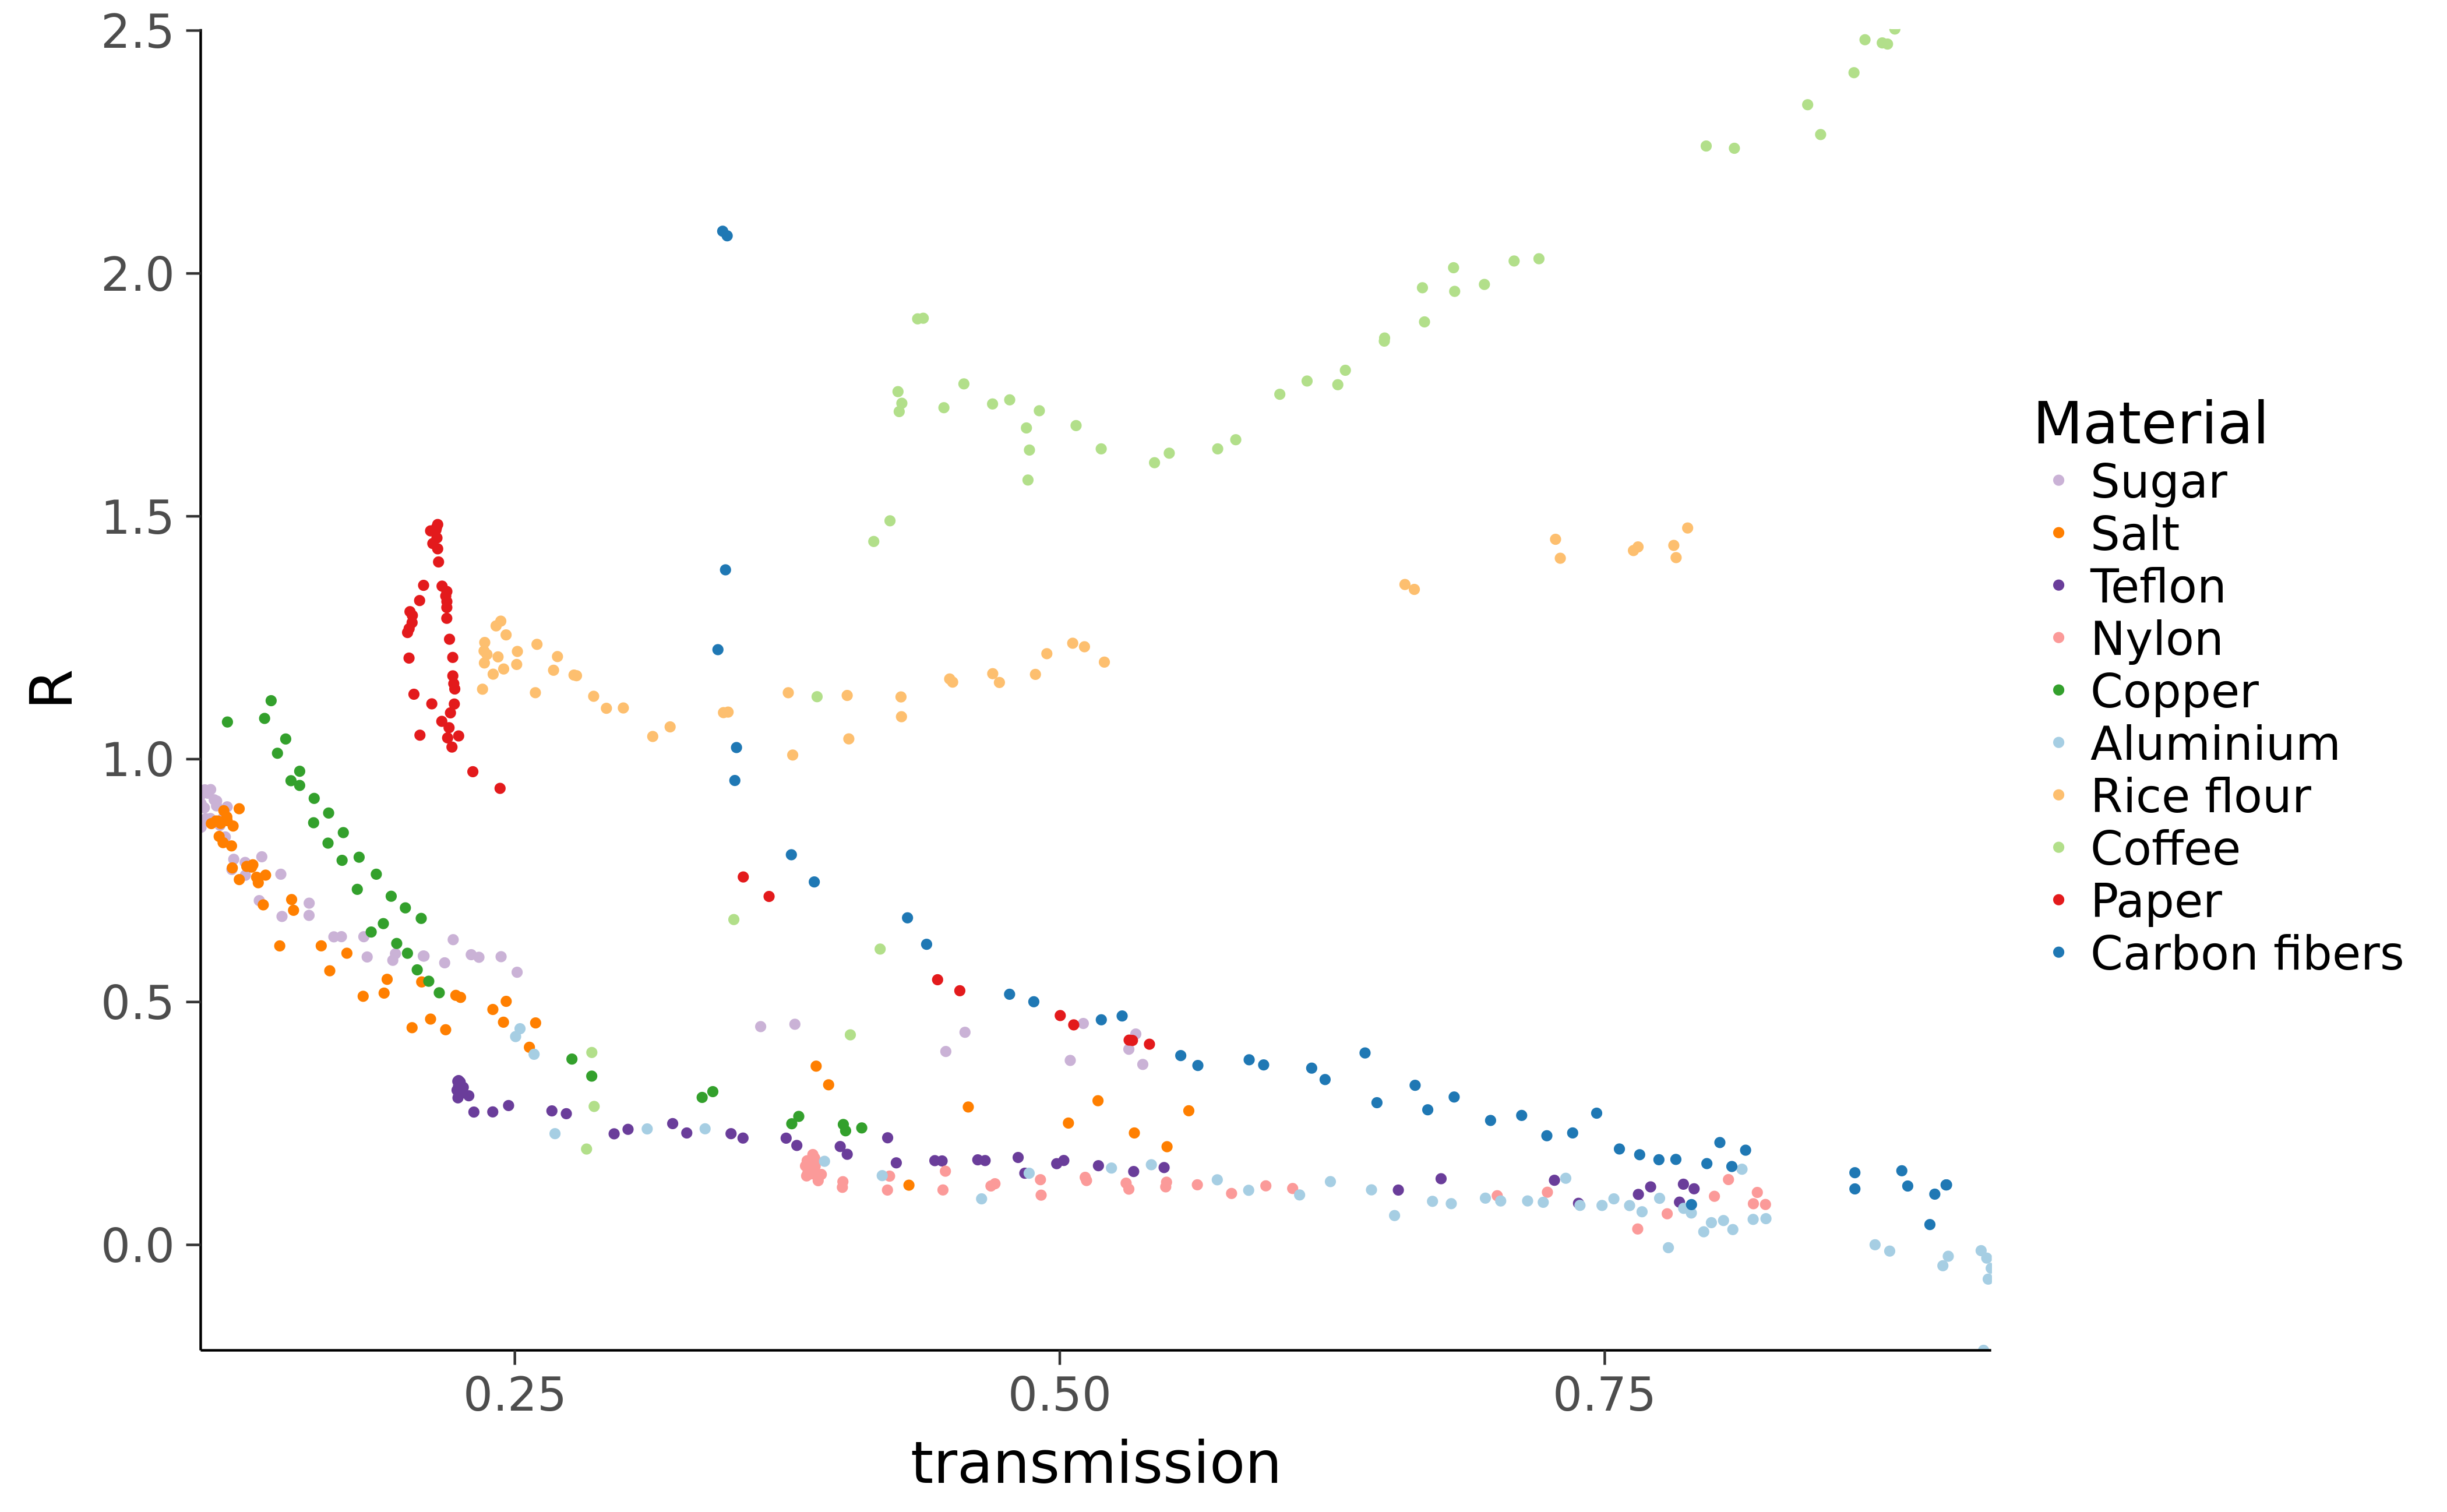
\includegraphics[width=\textwidth]{gfx/powders-aggregated.png}
    \caption{Ratio $R = \log(B) / \log(A)$ as a function of sample
    thickness, indicated by X-ray transmission, for different materials.}
    \label{fig:powders}
\end{figure}

The results at this stage are mainly qualitative in nature, as the samples
are very heterogeneous and contain particles of different sizes, but suggest
that powders have a stronger dark field signal than homogeneous samples,
thus indicating that further investigations, presented in
chapter~\ref{ch:lung-dark-field}, should be carried out to determine a more
precise model.
